\documentclass[authoryear,preprint,review,12pt]{elsarticle}
\usepackage[utf8x]{inputenc}
\usepackage{rotating}
\usepackage{tablefootnote}
\usepackage[a4paper, total={6.5in, 10.5in}]{geometry}
\usepackage[round]{natbib}
\bibliographystyle{plainnat}
\usepackage{filecontents}
\usepackage{lscape}
\usepackage{lipsum}
\usepackage{booktabs}
\usepackage{tabularx}
\usepackage{threeparttable}
\usepackage[font=scriptsize,labelfont=bf]{caption}
\usepackage[font=scriptsize,labelfont=bf]{subcaption}
\usepackage [autostyle, english = american]{csquotes}
\MakeOuterQuote{"}
\captionsetup[figure]{font=scriptsize}
\captionsetup[table]{font=scriptsize}
\usepackage{adjustbox}
\usepackage{graphicx}
\usepackage{amsmath}
\usepackage{hyperref}
\usepackage{setspace}
\usepackage{float}
\usepackage{array}
\usepackage{csvsimple}
\usepackage{threeparttable}
\setlength{\tabcolsep}{9pt}
\renewcommand{\arraystretch}{1.2}
\usepackage{pgfplotstable}
\pgfplotsset{compat=1.18}
\usepackage{array, multirow,makecell}
\newcolumntype{R}[1]{>{\raggedleft\arraybackslash }b{#1}}
\newcolumntype{L}[1]{>{\raggedright\arraybackslash }b{#1}}
\newcolumntype{C}[1]{>{\centering\arraybackslash }b{#1}}
\usepackage{wrapfig, blindtext}
\usepackage{booktabs} % For \toprule, \midrule and \bottomrule
\usepackage{siunitx} % Formats the units and values
\hypersetup{colorlinks=true,
    linkcolor=blue,
    filecolor=blue,      
    urlcolor=blue,
    citecolor=blue
    }
\urlstyle{same}
\onehalfspacing
\usepackage{graphicx}
\graphicspath{ {./images/}}
\usepackage{placeins} 


\begin{document}


\begin{frontmatter}


\title{Asylum seekers integration and local economies: evidence from Italian refugees reception centres}
\author[inst1]{Matteo Caruso}
\author[inst2]{Giuseppe Migali}
\affiliation[inst1]{organization={Department of Economics, Lancaster University Management School, Lancaster University},
             city={Lancaster},
             postcode={LA1 4YX},
             country={UK}}
\affiliation[inst2]{organization={Department of Economics, Law, and Sociology, Magna Graecia University}, city={Catanzaro},  country={Italy}}
 \date{}




\begin{abstract}
 
\noindent
This paper studies the impact of different types of Italian Asylum Seeker Reception Centres (ASRC) on Italian municipalities' economies.\ First, we analyse the impact of a refugee center on local spending, differentiating between centers with integration courses (SAI) and emergency centers that do no provide similar services (CAS).\ We do not find variations in the municipality's total spending, although there is evidence of a change in its composition.\ For the former, with find an increase in social spending and a modest decrease in other expenditure.\ For the CAS centers, we find more expenditure on local police and education, with a decrease on culture and economic development.\ As a second step, we explore the impact of these centers on local elections.\ We find a positive consistent correlation between the opening of the CAS (emergency) center and a change of the mayor afterwards.\ For the SAI (integration-oriented) centers there seems to be no significant impact on the election.\ 
\end{abstract}


\begin{keyword}
Asylum seekers reception centres \sep public finances \sep education \sep migration \sep local investments

\JEL K37 \sep H52 \sep H71 \sep H72 \sep 015
\end{keyword}



\end{frontmatter}

\section{Introduction}

\noindent
The problem of refugees has been a hot topic within the European Union for many years, especially for the Mediterranean countries, such as Italy, Greece, and Spain.\ The global political scenario in the past decades has been strongly influenced by the problem of illegal migration, both in the U.S. and Europe \citep{bracco2018}.\ Italy, for its strategic position, has been for several years at the centre of this debate, for being often 'the first country of entry', receiving most of the refugees from North Africa.\ In 2017, Italy was the second EU country, after Germany, for the number of asylum applications \citep{campesi2018}.\\

\noindent
We study the Italian reception system for asylum seekers and its effects on local finances.\ We focus on two different types of reception systems present on the territory, Integrated Reception System (SAI) centers and Centers of Extraordinary Reception (CAS).\ While the former is based on municipalities' cooperation and provides services for integration and education (e.g. language courses, legal counselling), the latter comes from the central government and does not usually provide the same services.\ From our analysis, we find opposite and heterogeneous effects of the two systems on local public finances, controlling for political, demographic, and economic variables.\ More precisely, while SAI centers increase local public expenditure from the hosting municipality, especially on social services, CAS facilities seems to be correlated with negative expenditure on socially relevant acitivies, such as culture, environment, and economic development.\ These difference in types of centers also seem to provide different impact on local elections.\ We believe that these different effects are a result of the different type of governance of the center.\ SAI centers are own by the municipality, managed by a local NGOs, and are mostly funded by the central government.\ CAS centers are government-run and their management can be assigned to both NGOs and private actors.\ The municipality where the facility is placed is not actively involved in the project.\ This might spur hostile sentiments from the local community, where the center is perceived as government-imposed and do not provide any type of integration of the refugees with the locals.\ This may influence local governments' spending choices.\\ 

\subsection*{Literature Review}

\noindent
While most of the literature and the political debate focus on the economic impact of migration, there is less attention to the specific case of refugees and asylum seekers and how they differ from economic or voluntary migrants \citep{becker2019}.\ According to the United Nations Geneva Convention, a refugee is any person who \textit{"owing to a well-founded fear of being persecuted for reasons of race, religion, nationality, membership of a particular social group or political opinion, is outside the country of his nationality and is unable or, owing to such fear, is unwilling to avail himself of the protection of that country"} \citep{convention1951}.\ Differently from the economic migrants, due to the impossibility of returning to their own home country, refugees may have different incentives with respect to social and cultural integration \citep{dustmann2017}.\ They may also differ in terms of short- and long-term effects on the labour market \citep{ruiz2018} or with respect to other social outcomes, such as education \citep{bauer2013, becker2020} or health \citep{bauer2017}.\\ 

\noindent
With respect to the hosting communities, forced migration may have different impacts both on private and public finances.\ \cite{chevalier2023} found an increase in local public spending for welfare and education due to a large-scale inflow of expelled Germans after WWII into West Germany.\ Similarly, \cite{ruist2015} shows how, compared to economic migrants, refugees in Sweden have a negative net impact on public finances, with the Swedish public sector redistributing around 1\% of GDP to the refugee population, through social spending on welfare and health.\ In contrast, \cite{Mahia2020TheApproach} results point to a positive impact on Turkey's GDP of Syrian refugees of approximately 2\% in the short-term and 4\% in the long term.\\


\noindent
Given the public nature of the phenomenon, much attention has been given to governments' approaches to deal with refugees reception and integration into local communities and societies.\ Notwithstanding the historically national aspect of this issue, considered as a horizontal decision-making, EU integration promoted instead a vertical approach since its policies in the 1980s and 1990s \citep{guiradon2000}, involving multiple levels of governance, both supra- and sub-national.\ While there is still no clear definition of multi-level governance (MLG) in the literature \citep{caponio2018}, it is possible to define MLG as a joint coordination between different levels of government, without a net dominance of one level on the other \citep{scholten2016}.\ This is different from other forms of governance, such as centralist (top-down) or localist (bottom-up), where cooperation and interactions are mostly absent \citep{scholten2018}.\ Other than the vertical perspective of the MGL, more recent research focused on its horizontal feature, involving not only coordination between central and local governments, but also exploring the role that nonpublic actors, i.e.\ NGOs and charity associations, have in addressing asylum seekers reception \citep{ambrosini2021}.\ Drawing from this literature, we decline these different types of governance in Italy's reception systems to assess their different impact on local economies.\ We compare Integrated Reception Centers (i.e. SPRAR or SAI) with Centers of Extraordinary Reception (i.e. CAS).\ While the former represents a form of MLG with municipalities volunteering to adhere to the project \citep{campomori2020}, the second represents instead a top-down approach, where central government establishes and controls the center, without a particular role of the municipality involved \citep{marchetti2014}.\ In this paper, we explore the economic and social impact of these two approaches and provide empirical evidence for future policy recommendations.\\


\vspace{5pt}

\section*{Institutional background and Italy's legislation on refugees}

\subsection{The Protection System for Aslyum Seekers and Refugees (SPRAR) and the MLG approach}

\noindent
Italy's legislation regarding migration and asylum policies has been historically fragmented and based on an emergency approach, notwithstanding its structural feature \citep{marchetti2014}.\ The number of asylum seekers in Italy had a stable pattern until the 1990s, when Western European countries experienced a surge of migrants from East-Europe due to fall of the Berlin Wall and the Balkan crisis \citep{anci2005}.\ Moreover, the entry into force of the Dublin Convention in 1997 established the 'first entry principle', leaving the burden of asylum seekers identification and registration on first-entry countries such as Italy, Spain and Greece \citep{lott2023}.\ This created the need for Italy to establish a more homogeneous reception system for asylum seekers and migrants.\\

\noindent
In this early context, the Italian system started to develop different phases in the reception process.\ In 1995, the Puglia Law established \textit{First Aid and Assistance Centers} (CPSA), with a logic of first aid and assistance and that are located close to the arrival of the migrants (now often addressed as 'hotspots') \citep{ricardguay2019}.\ In the following years, they were later complemented by \textit{Identification Centers} (CIE) in 2002, developed into \textit{Reception Centers for Asylum Seekers} (CARA) in 2008 \citep{campesi2018}.\ The CARA centers represent the first-phase of reception with a 'containement' purpose.\ These facilities have the objective to identify illegal migrants and provide them with basic assistance (health and psychological), for a limited amount of time necessary to start the asylum procedure.\ These first-line centers are government-run and have been criticised for low quality standards and overcrowding \citep{ricardguay2019}.\ The second type follows a 'dispersal' approach, where NGOs and local municipalities cooperates to open small reception centers and projects across the whole country.\ They are the second-line reception facilities, where asyluym seekers are provided with social, legal, and health assistance, with the purpose of their social and economic integration \citep{catarci2016}.\ The first initial project in 1999, called 'Azione Comune' (Common Action), lasted from 1999 to 2000.\ It was then developed into the 'Programma Nazionale di Asilo' or PNA (National Asylum Programme) from 2001 to 2003, and then was finally institutionalised in 2002 with law n°189/2002 \citep{bossifini2002}, finally creating the \textit{Protection System for Aslyum Seekers and Refugees} (SPRAR).\ Through the collaboration between the Ministry of the Interior and ANCI (the National Association of Italian Municipalities), this system aims at establishing a decentralised network between Italian municipalities providing services to asylum seekers and refugees for education and integration \citep{anci2005}.\ The SPRAR approach, notwithstanding its limits, has been addressed by the UNHCR as a good reception system, for it provides integration and educational support at the individual level \citep{catarci2016}.\\ 

\vspace{5pt}

\noindent
SPRAR centers (now referred to as \textit{Integrated Asylum System} or SAI), represent a good example of MLG.\ Funding for the projects comes for the 80\% from the \textit{'National fund for asylum policies and services'}, established by the Ministry of the Interior using European funds, and for the 20\% from the local municipality's resources \citep{anci2005}.\ It is important to underline that the participation to the system is voluntary and the application comes directly from the municipality and that are strongly encouraged by the Ministry of the Interior \citep{campomori2020}.\ Nonetheless, even though the local authority is the actual owner of the single project, in most cases the management is delegated to solidarity organisations and associations from the third sector (e.g. NGOs providing services to refugees), which played a relevant in role in the previous informal system too \citep{anci2005}.\ In this most common scenario, the NGOs are chosen by the municipality to manage the facility and the activites on behalf of the municipality itself, becoming the actual manager of the center (\textit{"ente gestore")}.\ This is the "horizontal dimension" of MLG, where the cooperation between public and nonpublic actors (i.e. NGOs) is enhanced to to address humanitarian crisis \citep{ambrosini2021}.\\

\subsection{Centers of Extraordinary Emergency (CAS) and the centralist approach}

\noindent
The Italian reception system experienced additional pressure following the 'Arab Spring' in 2011 and the subsequent increase of asylum seekers crossing the Mediterranean sea in the following years \citep{campesi2018}.\ This new emergency led to the multi-level agreement between State, Regions and Local Authorities in 2014 establishing a parallel and exceptional system to address the crisis.\ This brought up the creation of \textit{Centers of Extraordinary Reception} (i.e. CAS), which are second-line reception centers set up by the Ministry of the Interior through its local representatives (\textit{'prefetture'}).\ Differently from the SPRAR, these centers do not require municipalities' approval, and their management can be out-sourced to both NGOs and private actors through public contracts' procedures \citep{ricardguay2019}.\ While for the opening of the SPRAR, municipalities are required to submit a project proposal, providing integration services above certain standards, CAS centers do not have to meet these criteria \citep{campesi2018}, with a more "bed, bath, and bread" approach \citep{campomori2020}.\ Given the nature of the centers and the crisis facing Italy, many municipalities opposed the opening of the centers in their own territory.\ Even though only a few of them were successful in blocking the opening of the CAS, the protests highlighted the municipality's opposition to the center and their refusal to cooperate for the social integration of the refugees \citep{campomori2020}.\ These centers represent a more centralist or top-down approach, where coordination between different levels of government is absent and the central authority is the one imposing its decision on the local one \citep{scholten2018}.\\ 

\noindent
We exploit the presence of both systems to evaluate their different impact on local economies, looking at both education and employment variables.\ We provide evidence of the opposite effects that integrated and non-integrated systems have on local economies.\\ 

\section*{Data and identification strategy}

\noindent
For the data regarding the ASRCs, we rely on the data provided by OpenPolis foundation, which collected data from the Ministry of the Interior and other institutional sources \footnote{Centri d'Italia: \url{https://centriditalia.it/home}}.\ Data for SAI and CAS centers includes the location of the facility, with the municipality's identification code (ISTAT), the starting and ending date of the project, the number of refugees hosted and the capacity of the facility itself.\ We integrated missing data with the reports by ANCI and the Ministry of the Interior \footnote{Rete SAI: \url{https://www.retesai.it/la-storia/}} and with data provided by \cite{proietti2022}\footnote{We are grateful to Davide Luca for the data and the support}.\ Their data involves also municipalities physical characteristics, such as surface, degree of urbanisation, etc.\ The data for the centers starts from 2001, although most of them were actually approved by the Ministry of the Interior only from 2006 \citep{marchetti2014}.\ We include those informal projects from 2002, although just a few municipalities were implementing them.\\  

\vspace{2pt}

\noindent
For what concerns data on municipalities' public finances, from 1998 to 2014, we make use of the data from the Department of Internal and Territorial Affairs, of the Ministry of the Interior\footnote{Department of Internal and Territorial Affairs: \url{https://finanzalocale.interno.gov.it/apps/floc.php/in/cod/4}}.\ We rely on the Minister of the Economy and Finance for the years from 2015 to 2021\footnote{OpenBilanci: \url{https://openbilanci.it}} \footnote{It is important to underline that municipalities were affected by a territorial reform which forced them to change the expenditure functions from 2015 \citep{bolgherini2016}.\ We run the same analysis in the pre-reform period (1998-2014) for SAI centers and in the post-reform period for both CAS and SAI (2015-2021), finding similar results.}.\ We use other covariates (e.g.\ as total, foreign, and African population, local elections and officials, municipality's tax base and number resident with an employee contract) from different ministerial sources such as the Department of Internal and Local Affairs\footnote{Department of Internal and Territorial Affairs: \url{https://dait.interno.gov.it/elezioni/open-data}}, and the Ministry of Economics and Finance\footnote{Department of Local Finances: \url{https://www.mef.gov.it/documenti-pubblicazioni/open-data/index.html}}.\\ 


\section*{Method}

\noindent
For the first part of the paper, we focus on the impact of refugee centers on local spending patterns, using a difference-in-difference approach with multiple treatments in different periods, following \cite{clarke2020}.\ We use both the never-treated and the not-yet treated as control groups, controlling for relevant observable characteristics, as total, foreign, and African population, as well as the tax base and the number of taxpayers with an employee contract.\ We also control for the presence of the other type of ASRC in the municipality (e.g.\ controlling for the presence of SAI in the CAS analysis and viceversa).\ Given the high number of observations in the control group, we restrict the untreated units using a propensity score matching (PSM) \citep{rubin1985} based on geographical characteristics (e.g. location, region and province, altitude, climate, etc.).\ Our assumption is that municipalities' location and climatic features may influence the choice of opening a refugee center but are not affected by the treatment itself in the post-treatment period \citep{Austin2011AnStudies}.\ For this first analysis, we end up having 773 treated municipalities matched with 743 controls.\\ 

\input{tables/pop_100000/descriptive stats cas.txt}


\section*{Results}

\subsection*{Effects of centers opening on public finances}
\normalsize

\noindent
This section presents the results for the first analysis, e.g.\ the impact of the opening of the refugee center on local public spending patterns.\ We restrict the analysis to the municipalities with populations smaller than than 100'000 people, to exclude metropolitan and large cities, for which the relevance of the centers are likely to be much smaller.\\

\noindent
For what concerns the SAI centers, as Figure \ref{fig:total_spending} shows, the model does not show any effects on total spending.\ Nonetheless, there seem to be relevant variations in spending patterns.\ The main effect is related to social services spending (Figure \ref{fig:social_services}).\ This does not come as a surprise as the refugee center requires relevant spending from the local administration, although the management is assigned to the NGO.\ More interesting, it is a possible substitution effect on other expenditures.\ In our case, spending on sport, free-time, and youth-related activities \footnote{For a more specific description of the expenditure, we refer to the National Association of Italian Municipalities (ANCI) report: \url{https://www.fondazioneifel.it/contabilita/item/download/1444_a4d1fd88f0e38b598046aba2fa08fa0f}} experience a significant reduction in the years after the opening of the center (Figure \ref{fig:sport}).\ These are expenditures that are likely to be the easiest to cut when needed, compared to other types of necessities, such as education and transport.\ Other expenditures do not seem to have significant changes.\\ 

\noindent
For what concerns the CAS centers, which are imposed by the central government following a more 'top-down' approach, the impacts on public spending are more evident.\ This could be also due to exogenous feature of the treatment for these municipalities.\ While for SAI centers the application to open the centers comes from the municipality itself, for CAS facilities most of the times the decision comes from the Ministry of the Interior.\ In these municipalities, we find an increase in the expenditures related to local police and education activities (Figures \ref{fig:caspolice} and \ref{fig:caseducation}).\ We also see a significant reduction on expenditures related to culture, economic development, and the environment (Figures \ref{fig:casculture}, \ref{fig:casecodev}, \ref{fig:casenvironment}).\ We believe that such changes are related to the perceived negative impact of the center on the local community, forcing the administration to increase the safety of the city through more local police and to increase the expenditure on local schools.\ More 'social oriented' expenditure, such as cultural, environmental, and economic development, seem to be the ones to be reduced instead.\\ 


\begin{figure}[!ht]
\fontsize{7.2}{7.2}\selectfont
    \centering
\caption*{Effect of CAS centers on municipalities' public spending}
    \begin{tabular}{@{}ccc@{}}
        \begin{minipage}[t]{0.32\textwidth}
            \centering
            \caption{Total spending}
            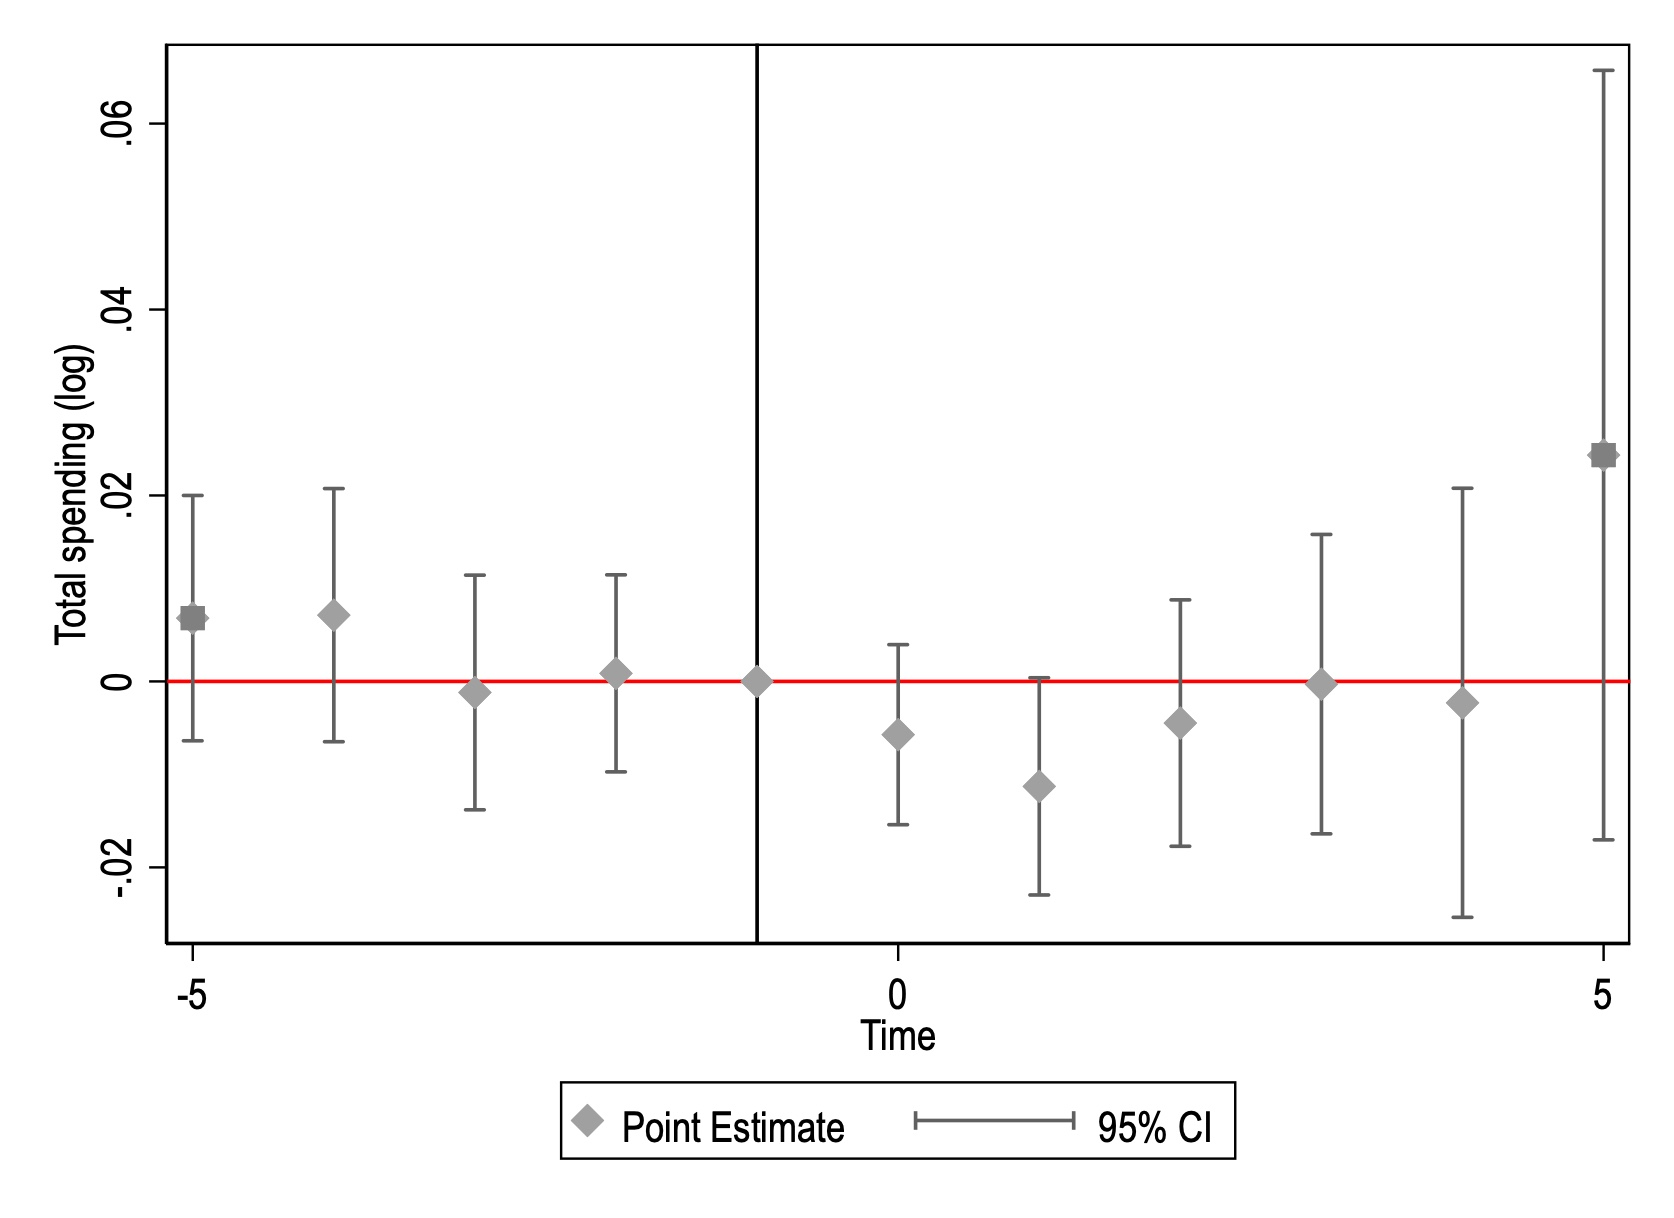
\includegraphics[width=\linewidth]{images/pop_100000/caseventdd_ln_q4tot_step1.jpg}
            \label{fig:castotal_spending}
        \end{minipage} &
        \begin{minipage}[t]{0.32\textwidth}
            \centering
            \caption{Sport}
            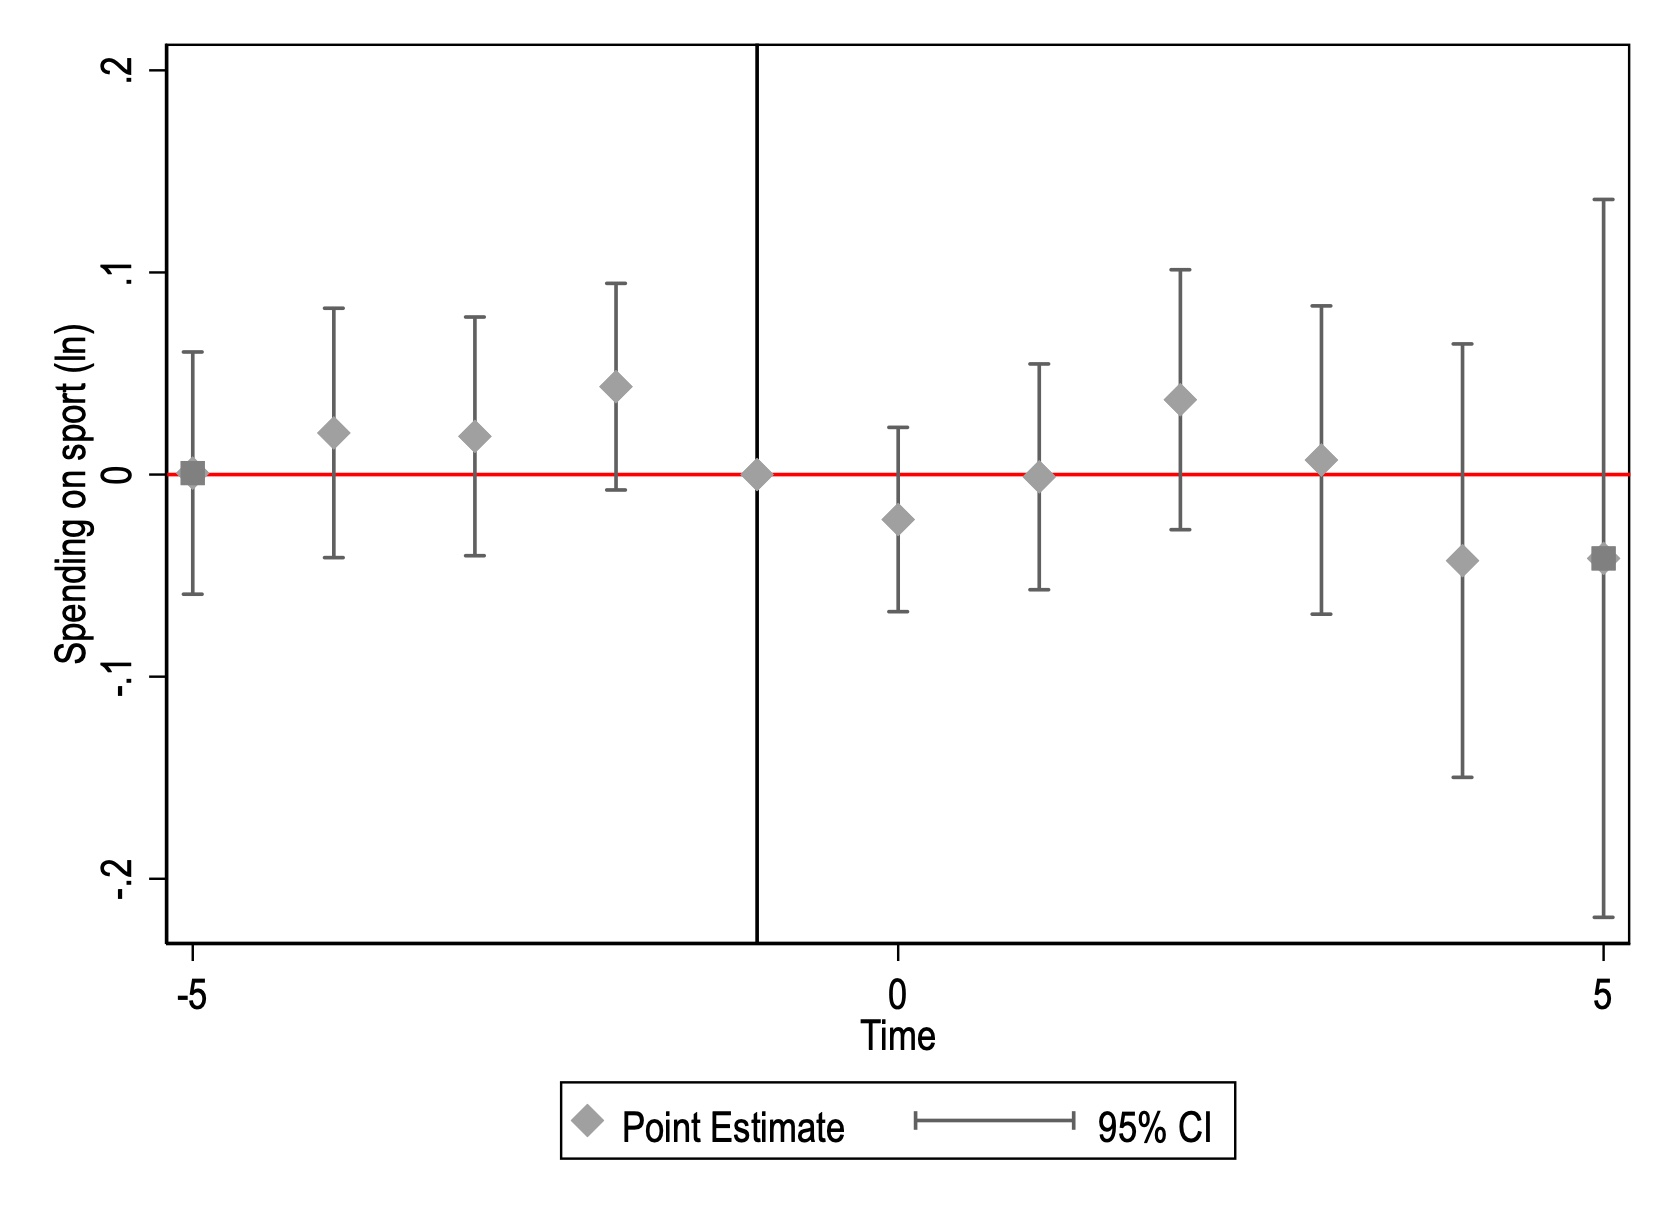
\includegraphics[width=\linewidth]{images/pop_100000/caseventdd_ln_q4_06_step1.jpg}
            \label{fig:cassport}
        \end{minipage} &
        \begin{minipage}[t]{0.32\textwidth}
            \centering
            \caption{Transport}
            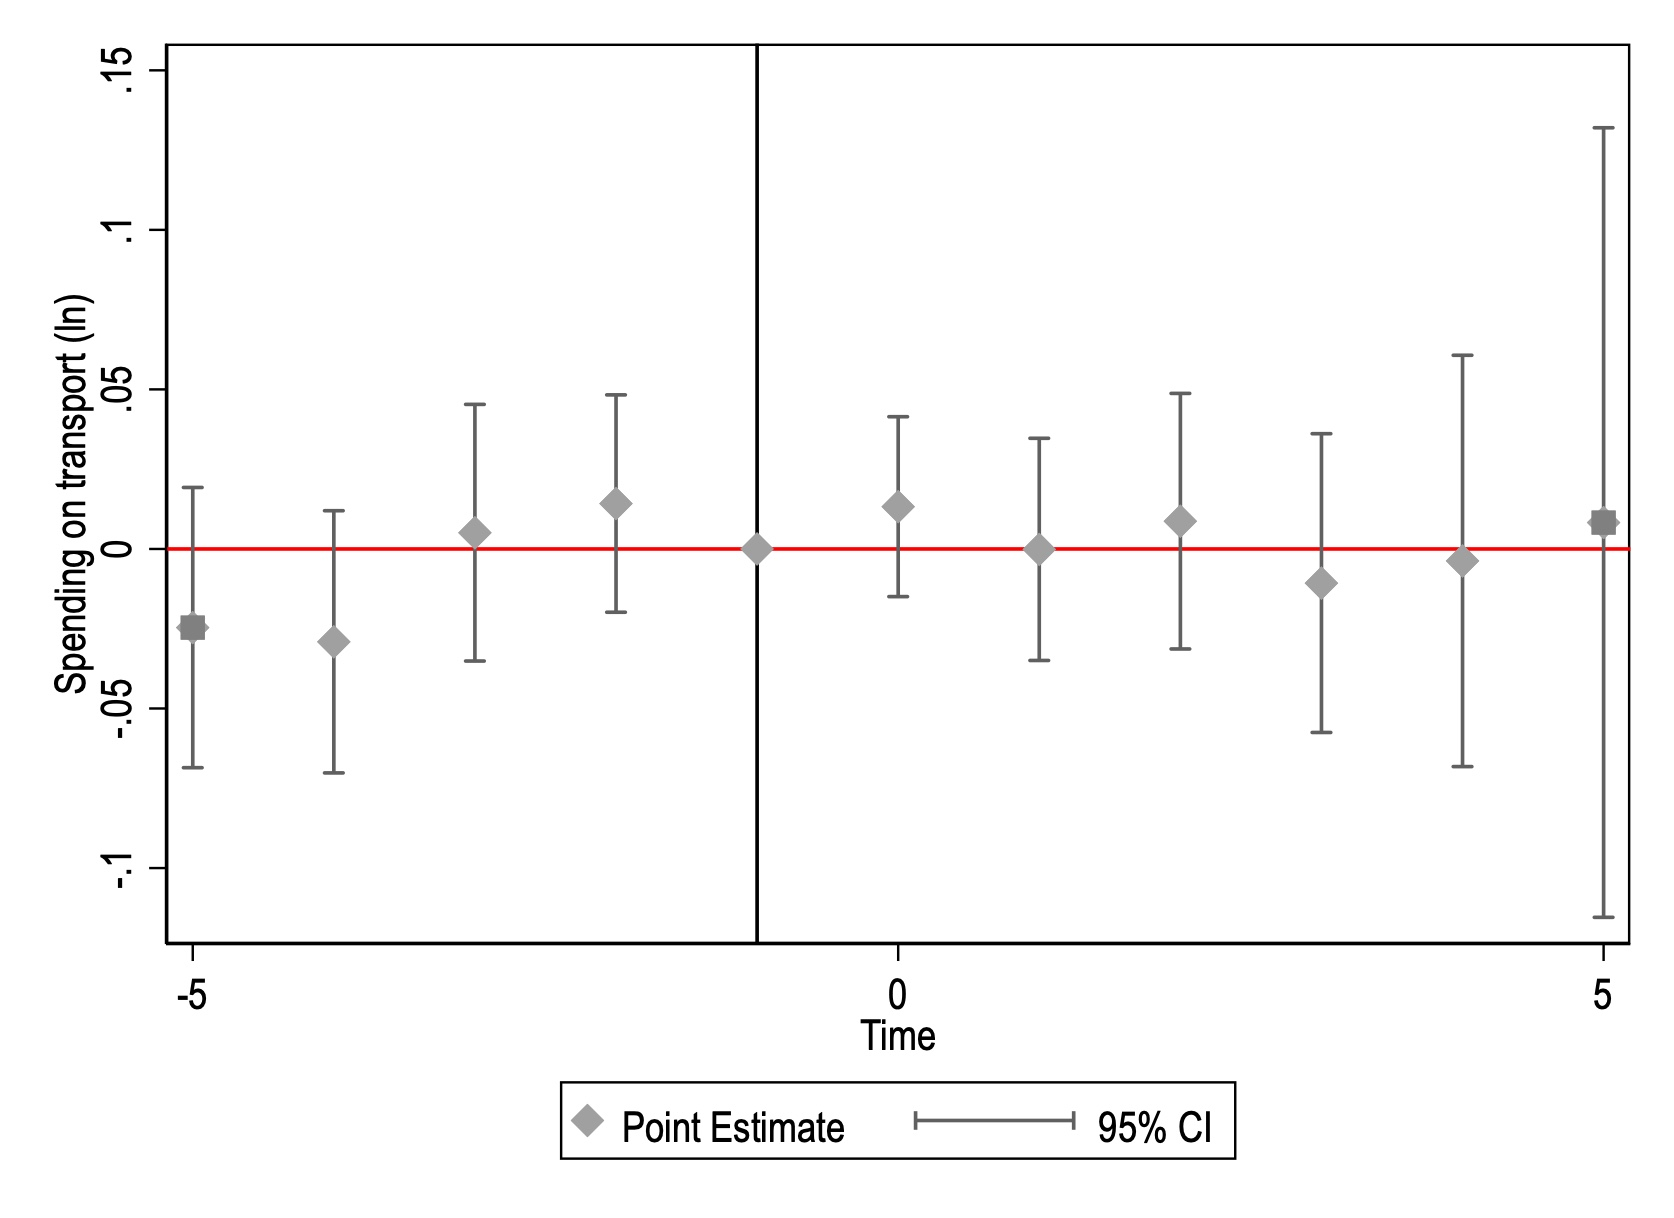
\includegraphics[width=\linewidth]{images/pop_100000/caseventdd_ln_q4_08_step1.jpg}
            \label{fig:castransport}
        \end{minipage} \\[10pt]

        \begin{minipage}[t]{0.32\textwidth}
            \centering
            \caption{Justice}
            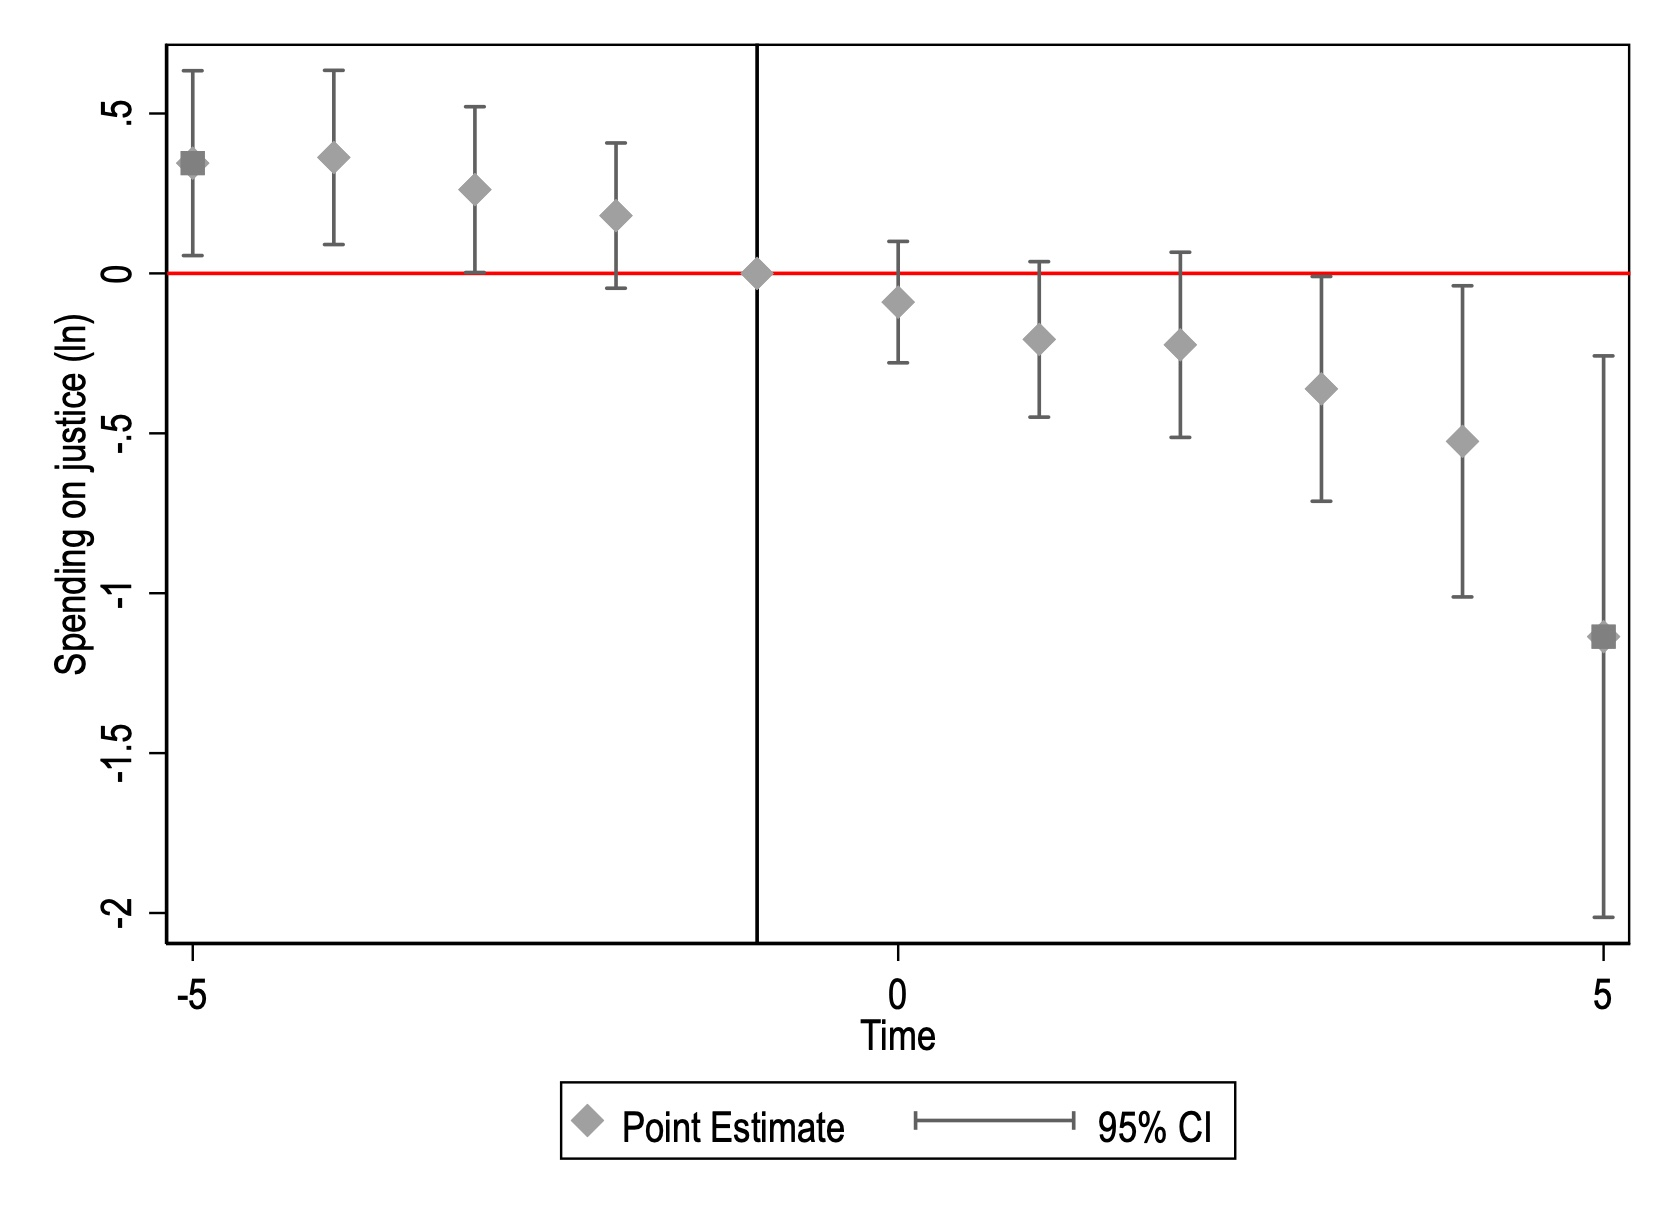
\includegraphics[width=\linewidth]{images/pop_100000/caseventdd_ln_q4_02_step1.jpg}
            \label{fig:casjustice}
        \end{minipage} &
        \begin{minipage}[t]{0.32\textwidth}
            \centering
            \caption{Police}
            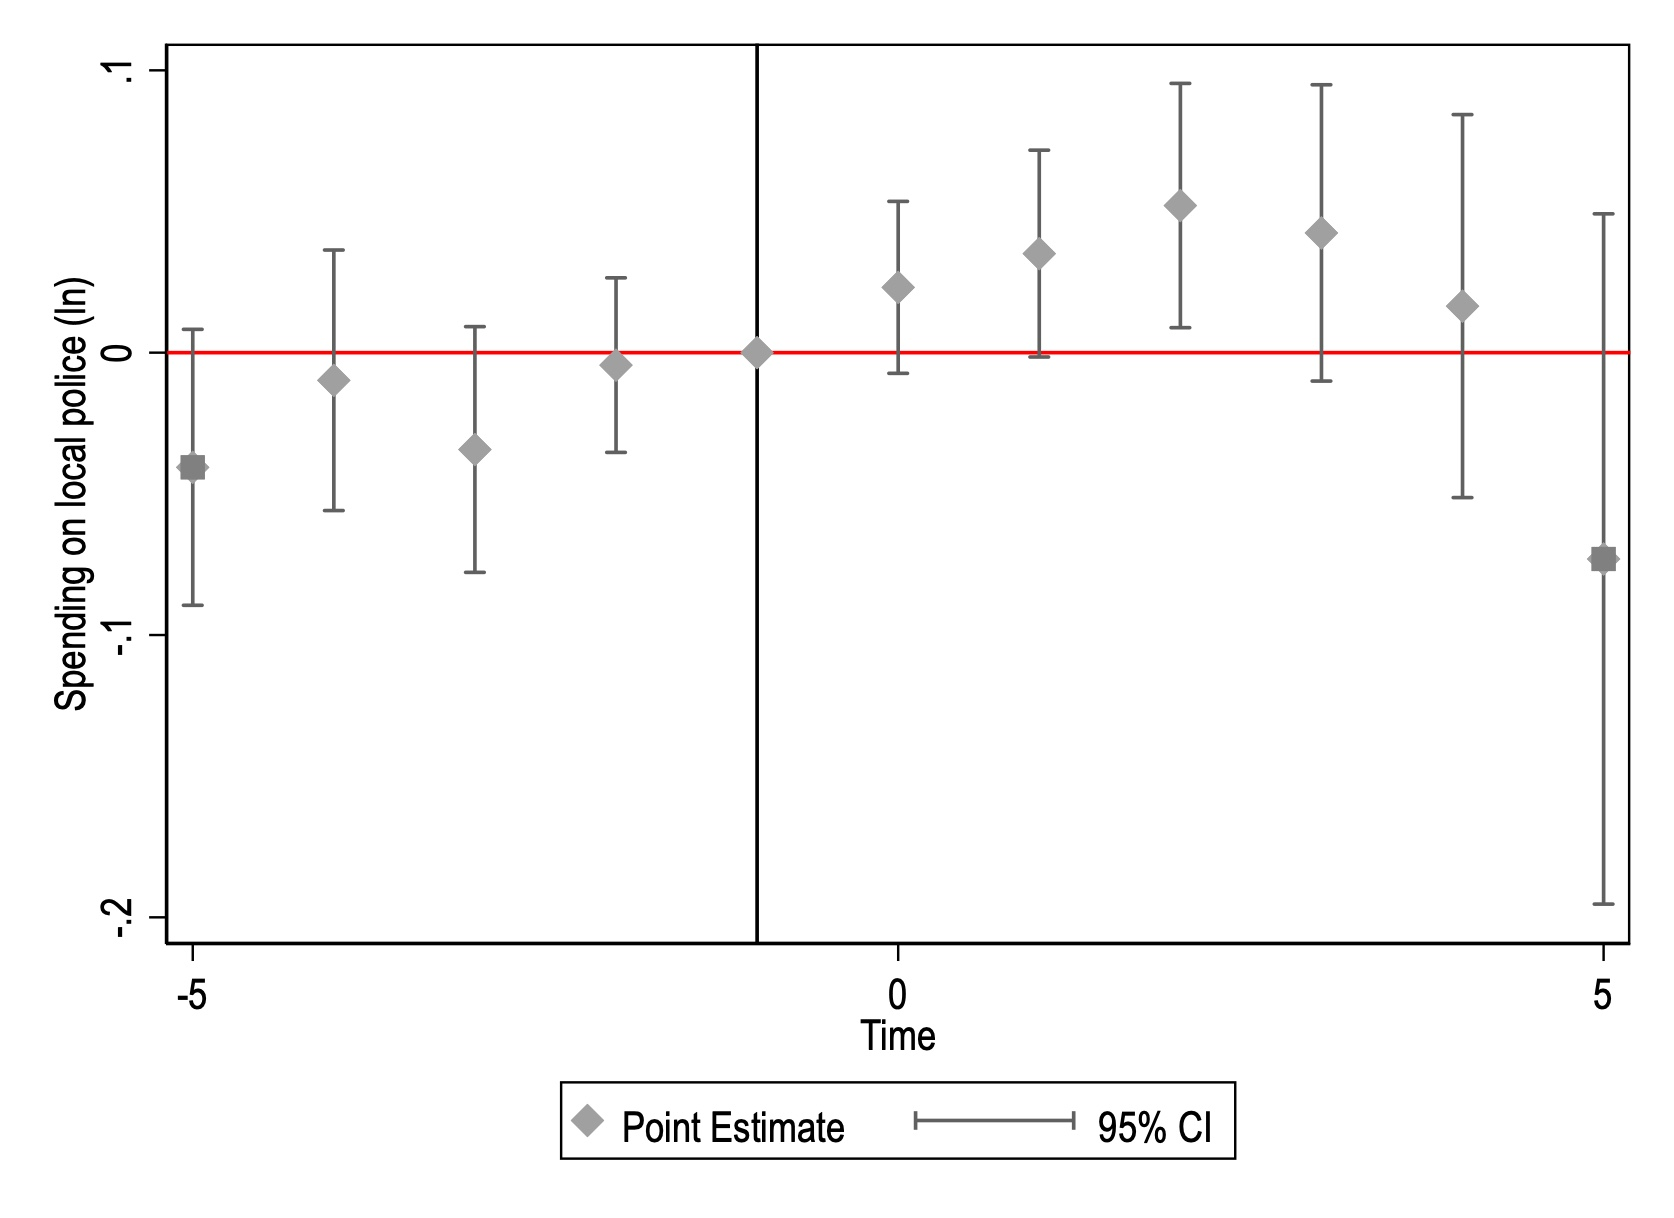
\includegraphics[width=\linewidth]{images/pop_100000/caseventdd_ln_q4_03_step1.jpg}
            \label{fig:caspolice}
        \end{minipage} &
        \begin{minipage}[t]{0.32\textwidth}
            \centering
            \caption{Culture, libraries, museums}
            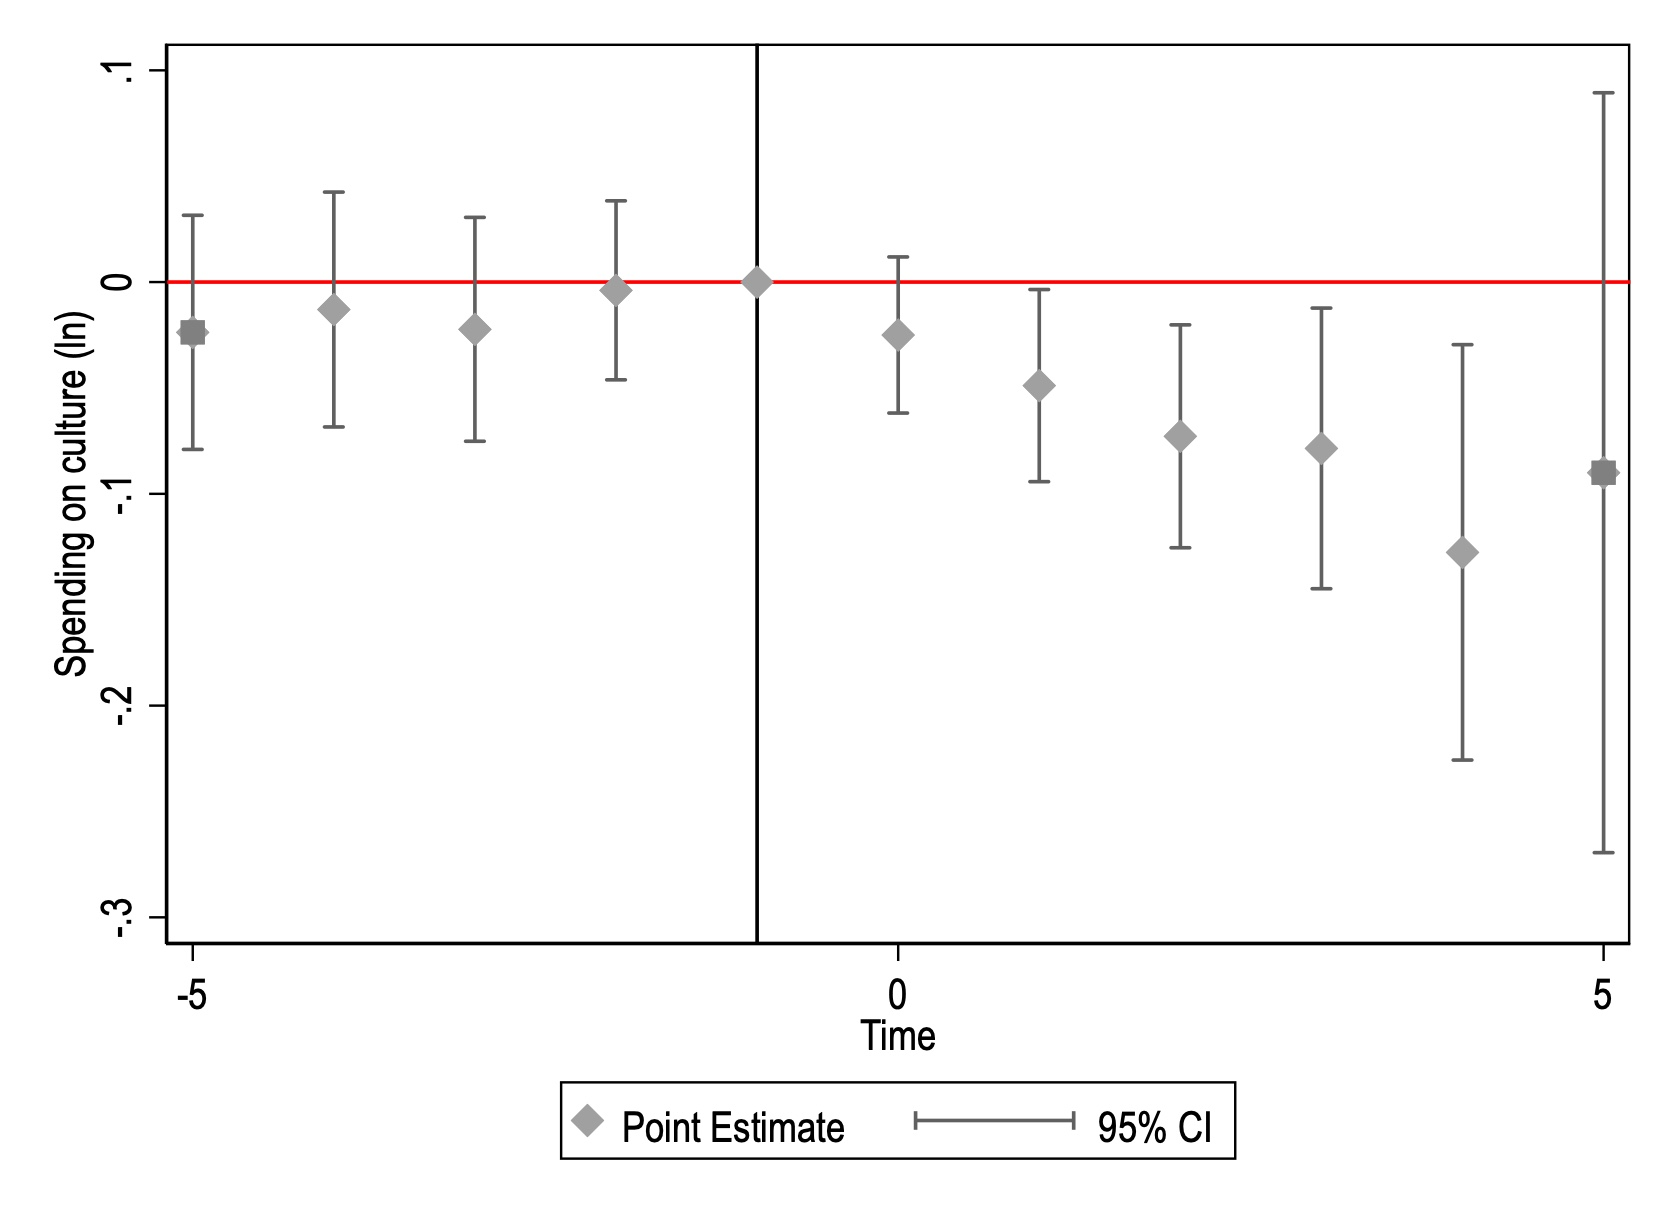
\includegraphics[width=\linewidth]{images/pop_100000/caseventdd_ln_q4_05_step1.jpg}
            \label{fig:casculture}
        \end{minipage} \\[10pt]

        \begin{minipage}[t]{0.32\textwidth}
            \centering
            \caption{Social services}
            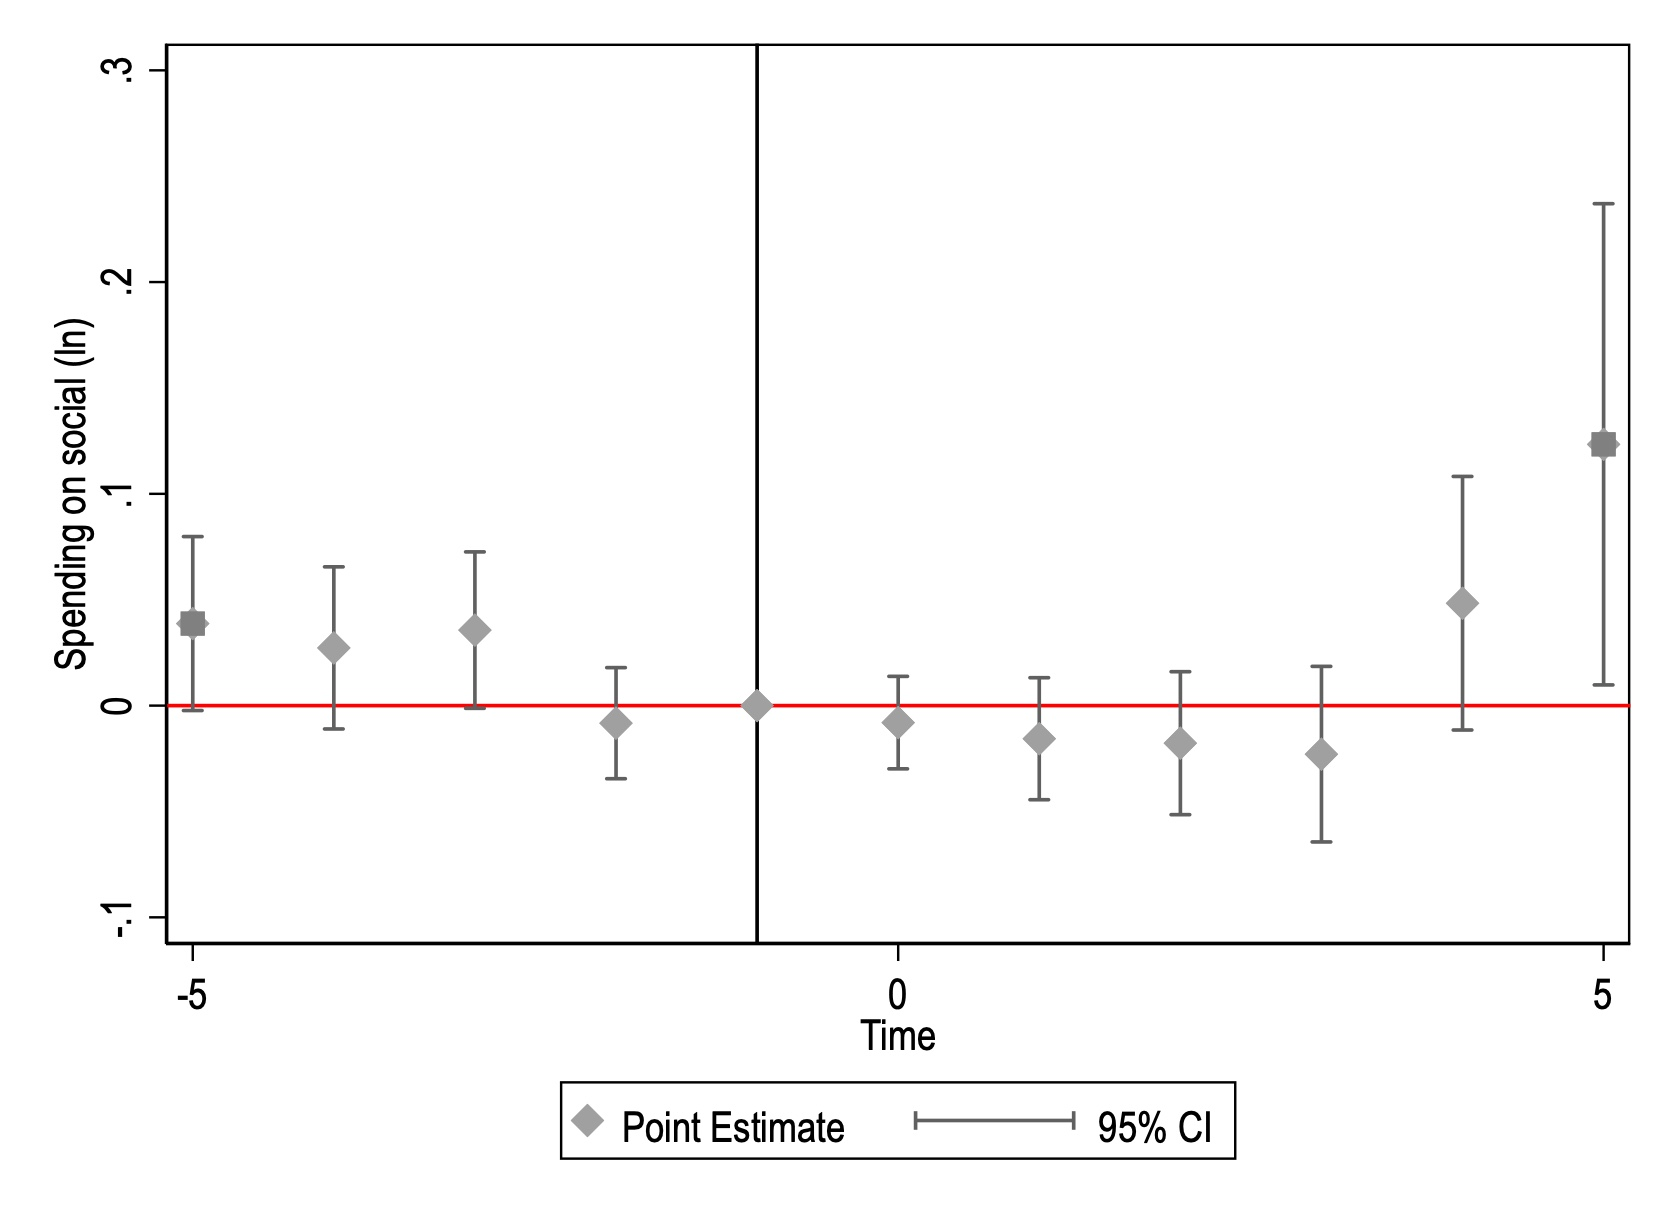
\includegraphics[width=\linewidth]{images/pop_100000/caseventdd_ln_q4_10_step1.jpg}
            \label{fig:cassocial_services}
        \end{minipage} &
        \begin{minipage}[t]{0.32\textwidth}
            \centering
            \caption{Education}
            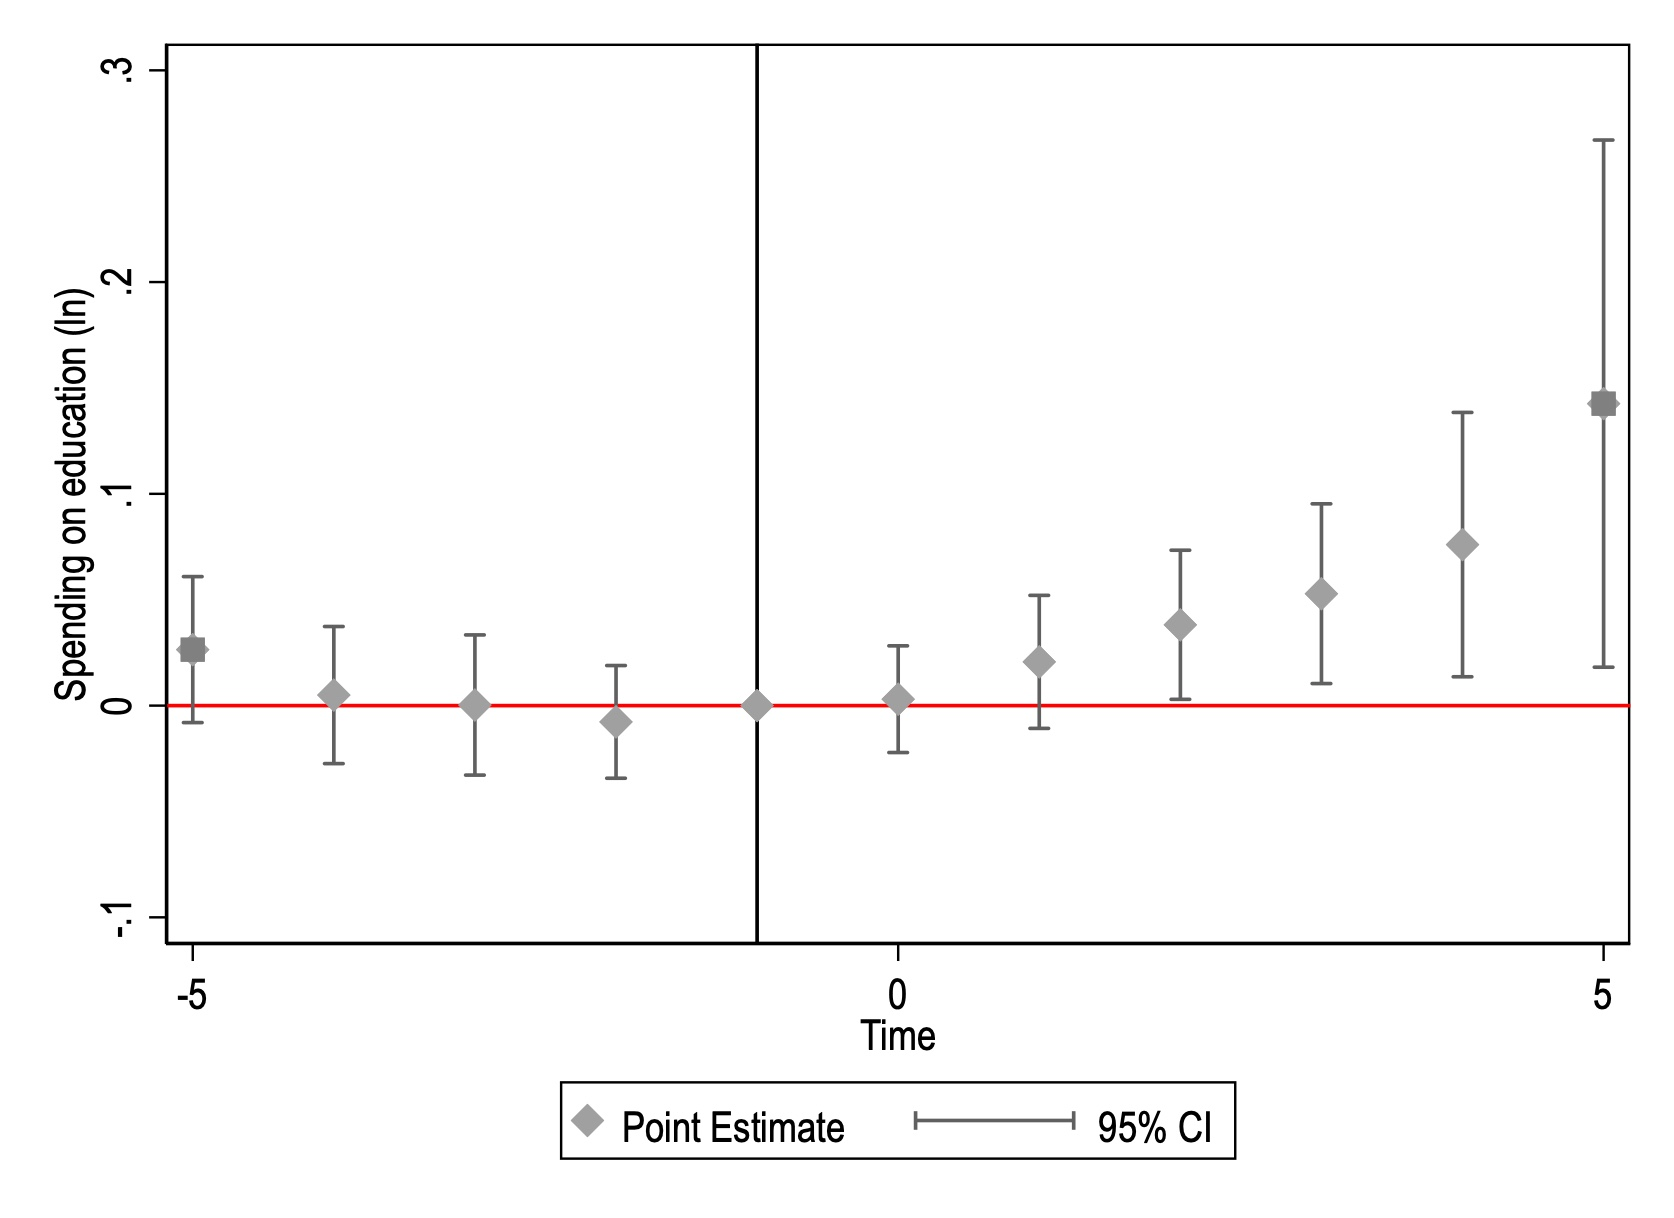
\includegraphics[width=\linewidth]{images/pop_100000/caseventdd_ln_q4_04_step1.jpg}
            \label{fig:caseducation}
        \end{minipage} &
        \begin{minipage}[t]{0.32\textwidth}
            \centering
            \caption{Economic development}
            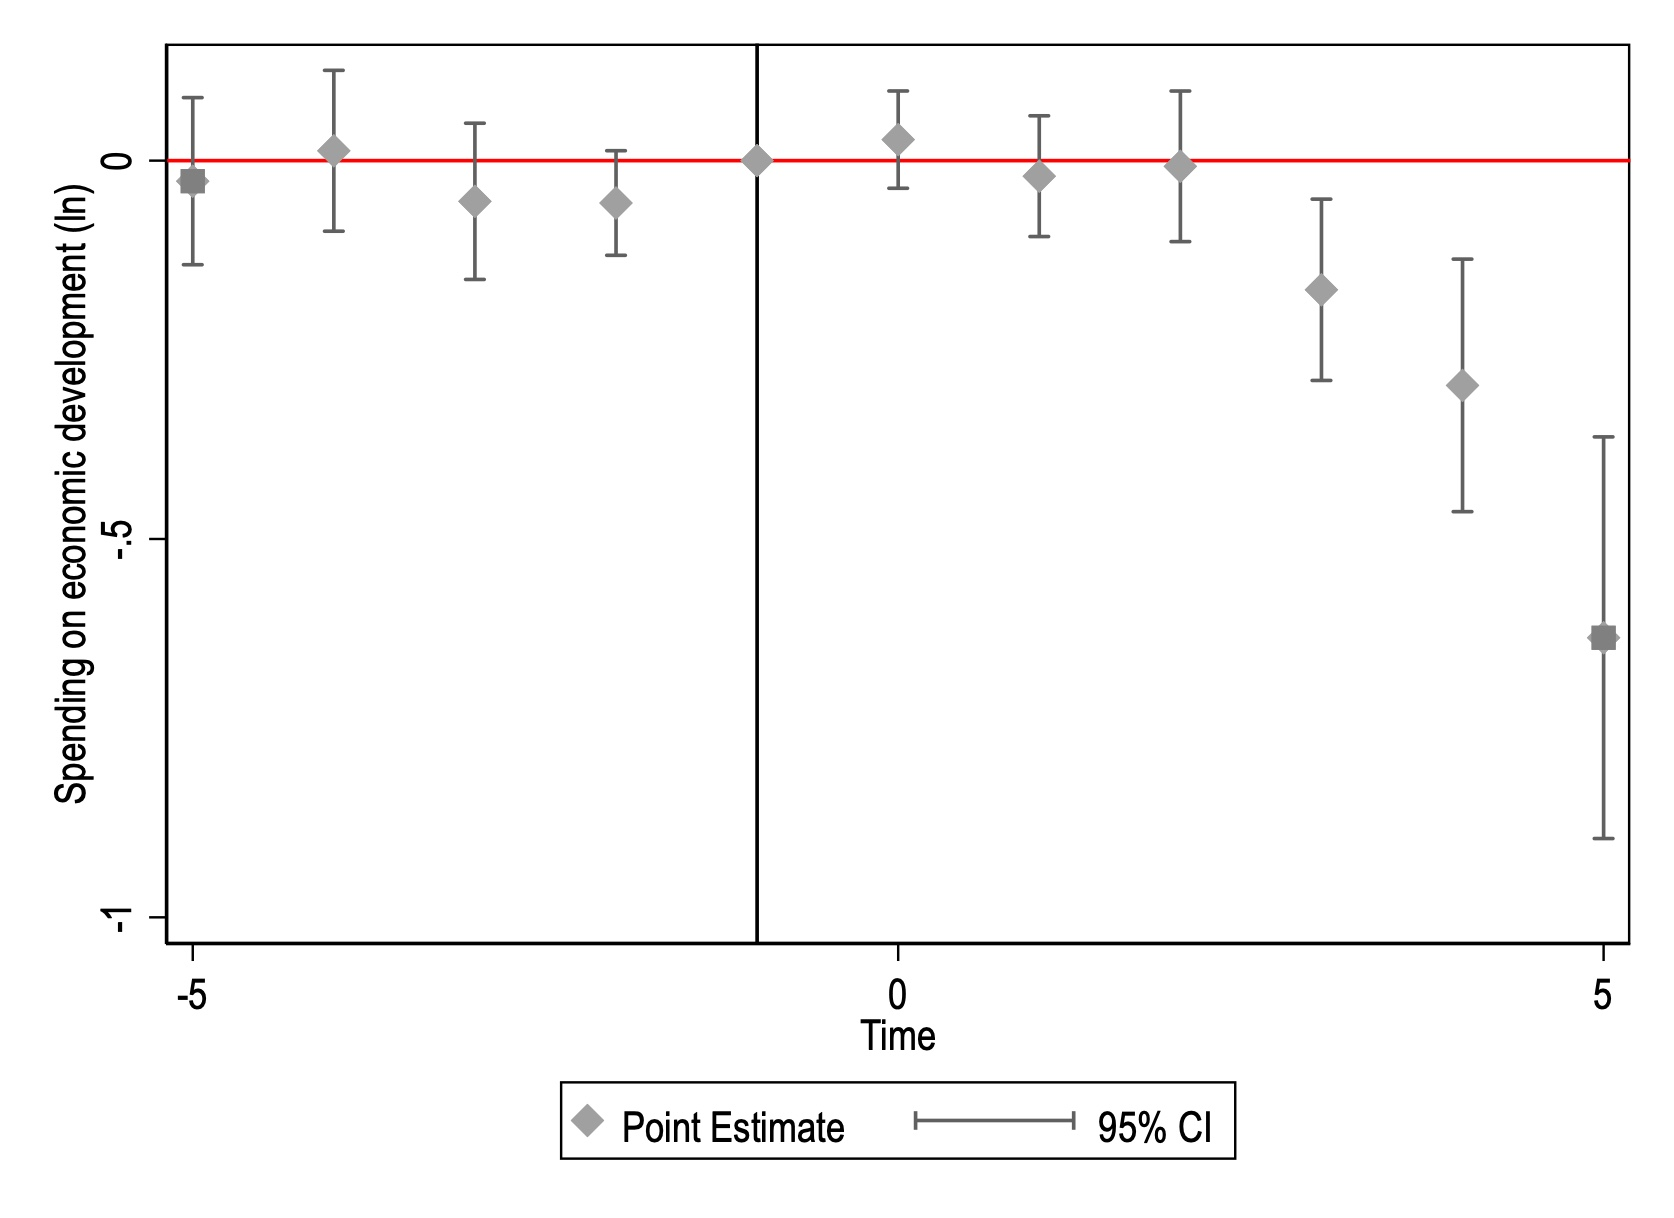
\includegraphics[width=\linewidth]{images/pop_100000/caseventdd_ln_q4_11_step1.jpg}
            \label{fig:casecodev}
        \end{minipage} \\[10pt]

        \begin{minipage}[t]{0.32\textwidth}
            \centering
            \caption{Production services}
            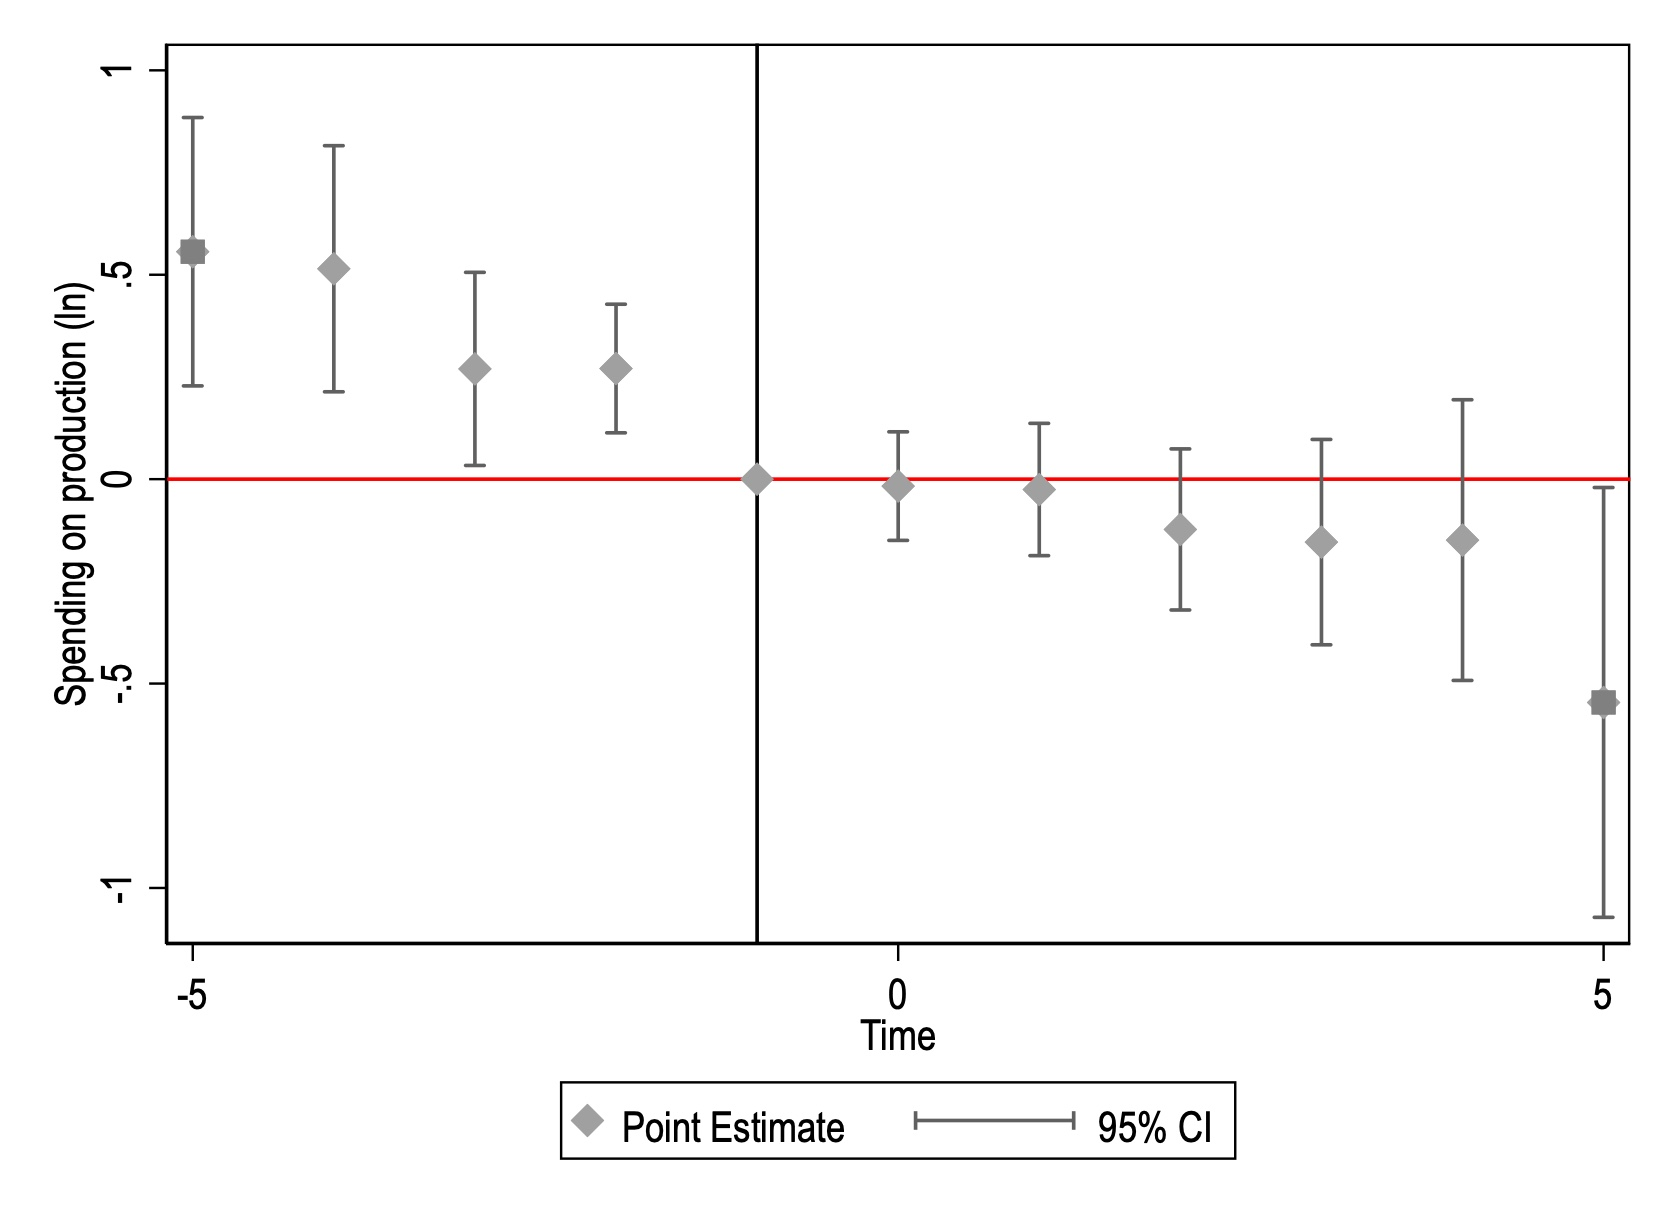
\includegraphics[width=\linewidth]{images/pop_100000/caseventdd_ln_q4_12_step1.jpg}
            \label{fig:cascproduction}
        \end{minipage} &
        \begin{minipage}[t]{0.32\textwidth}
            \centering
            \caption{Administrative services}
            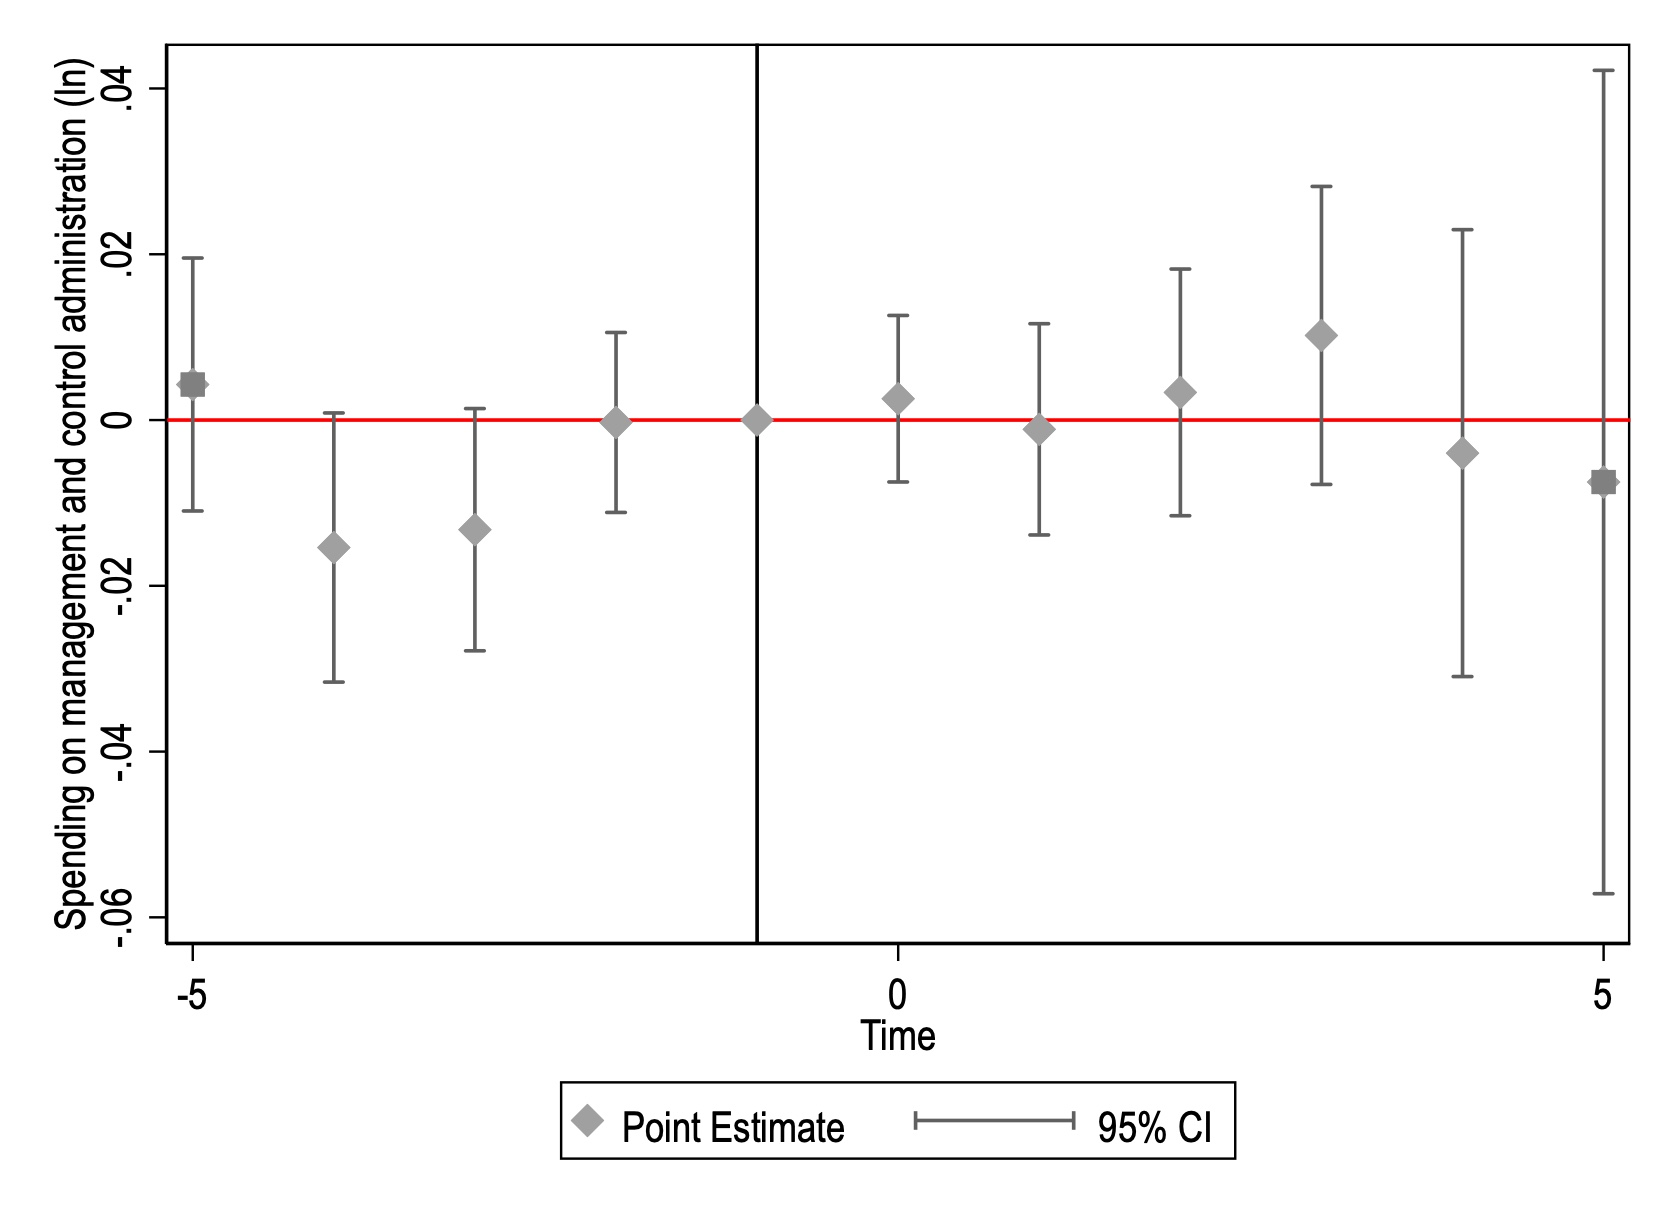
\includegraphics[width=\linewidth]{images/pop_100000/caseventdd_ln_q4_01_step1.jpg}
            \label{fig:casadministration}
        \end{minipage} &
        \begin{minipage}[t]{0.32\textwidth}
            \centering
            \caption{Environment, public parks, recycling}
            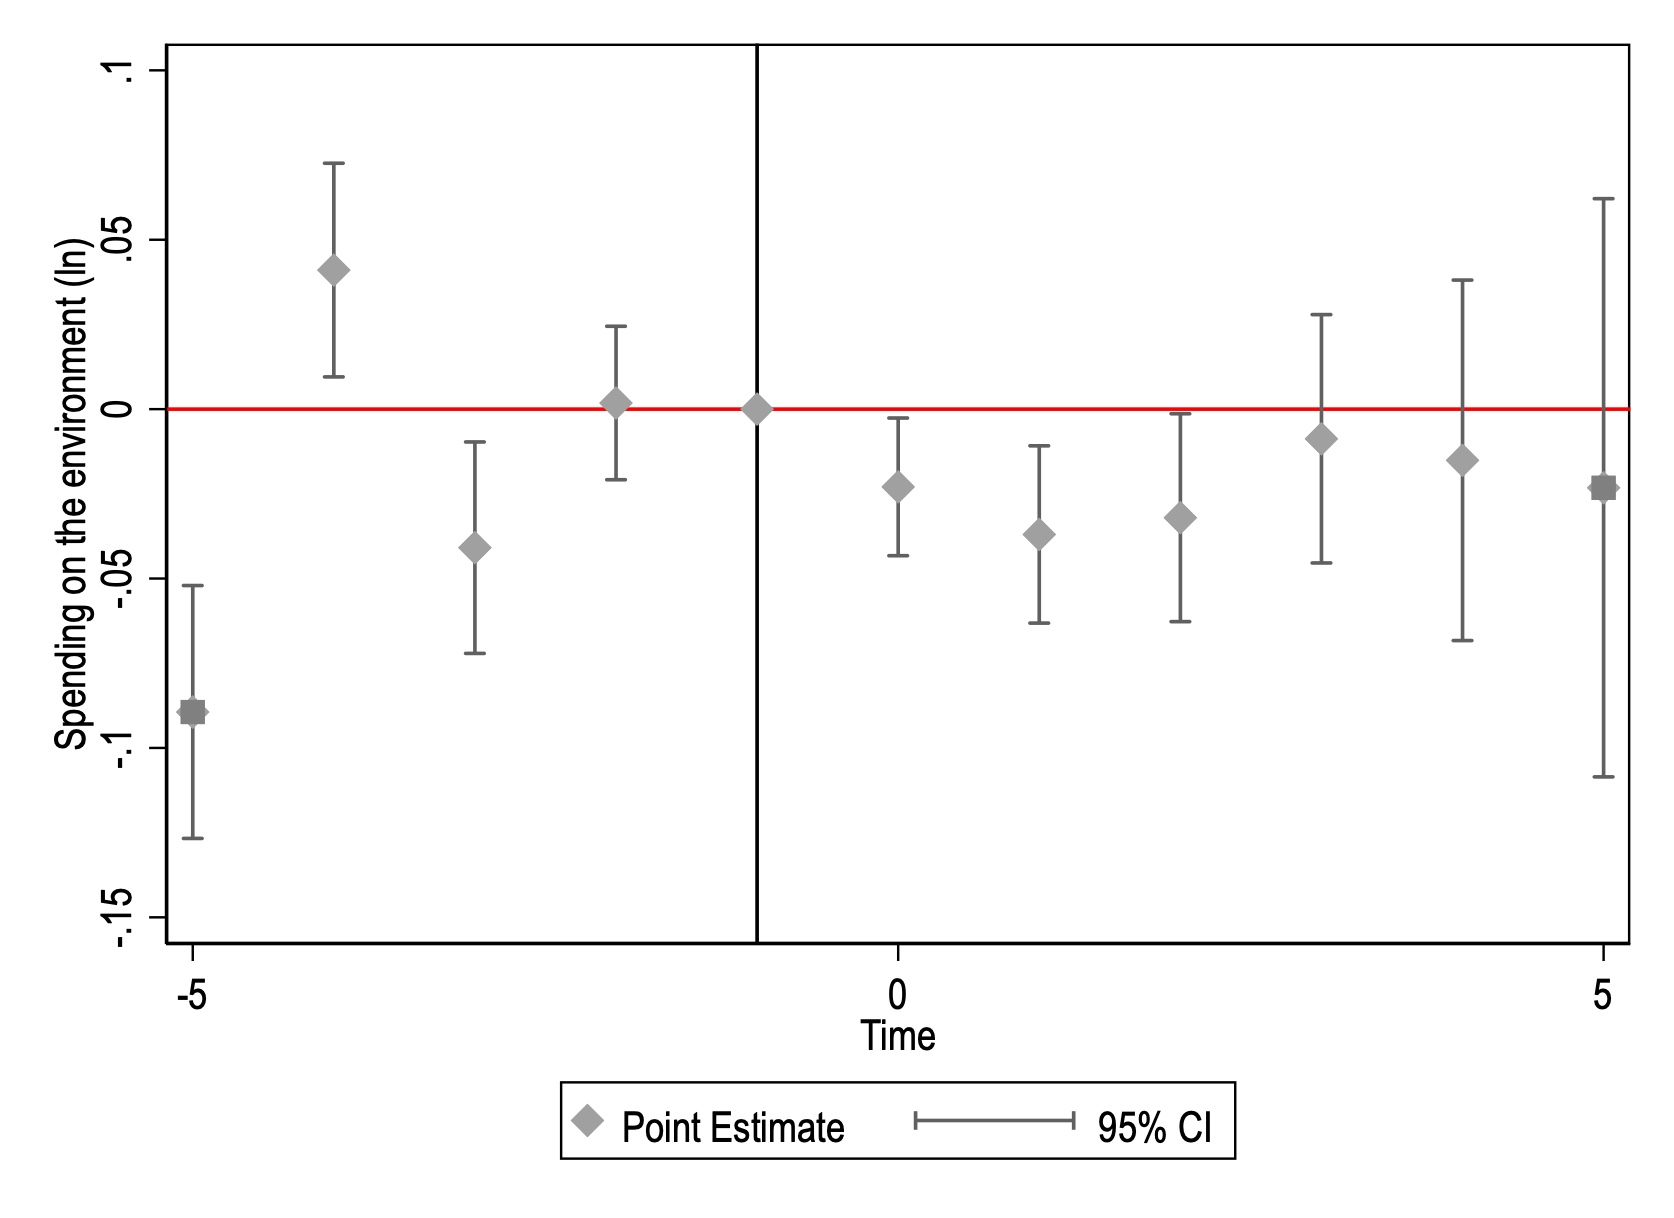
\includegraphics[width=\linewidth]{images/pop_100000/caseventdd_ln_q4_09_step1.jpg}
            \label{fig:casenvironment}
        \end{minipage}
    \end{tabular}
\end{figure}



\begin{figure}[!ht]
\fontsize{7.2}{7.2}\selectfont
    \centering
\caption*{Effect of SAI centers on municipalities' public spending}
    \begin{tabular}{@{}ccc@{}}
        \begin{minipage}[t]{0.32\textwidth}
            \centering
            \caption{Total spending}
            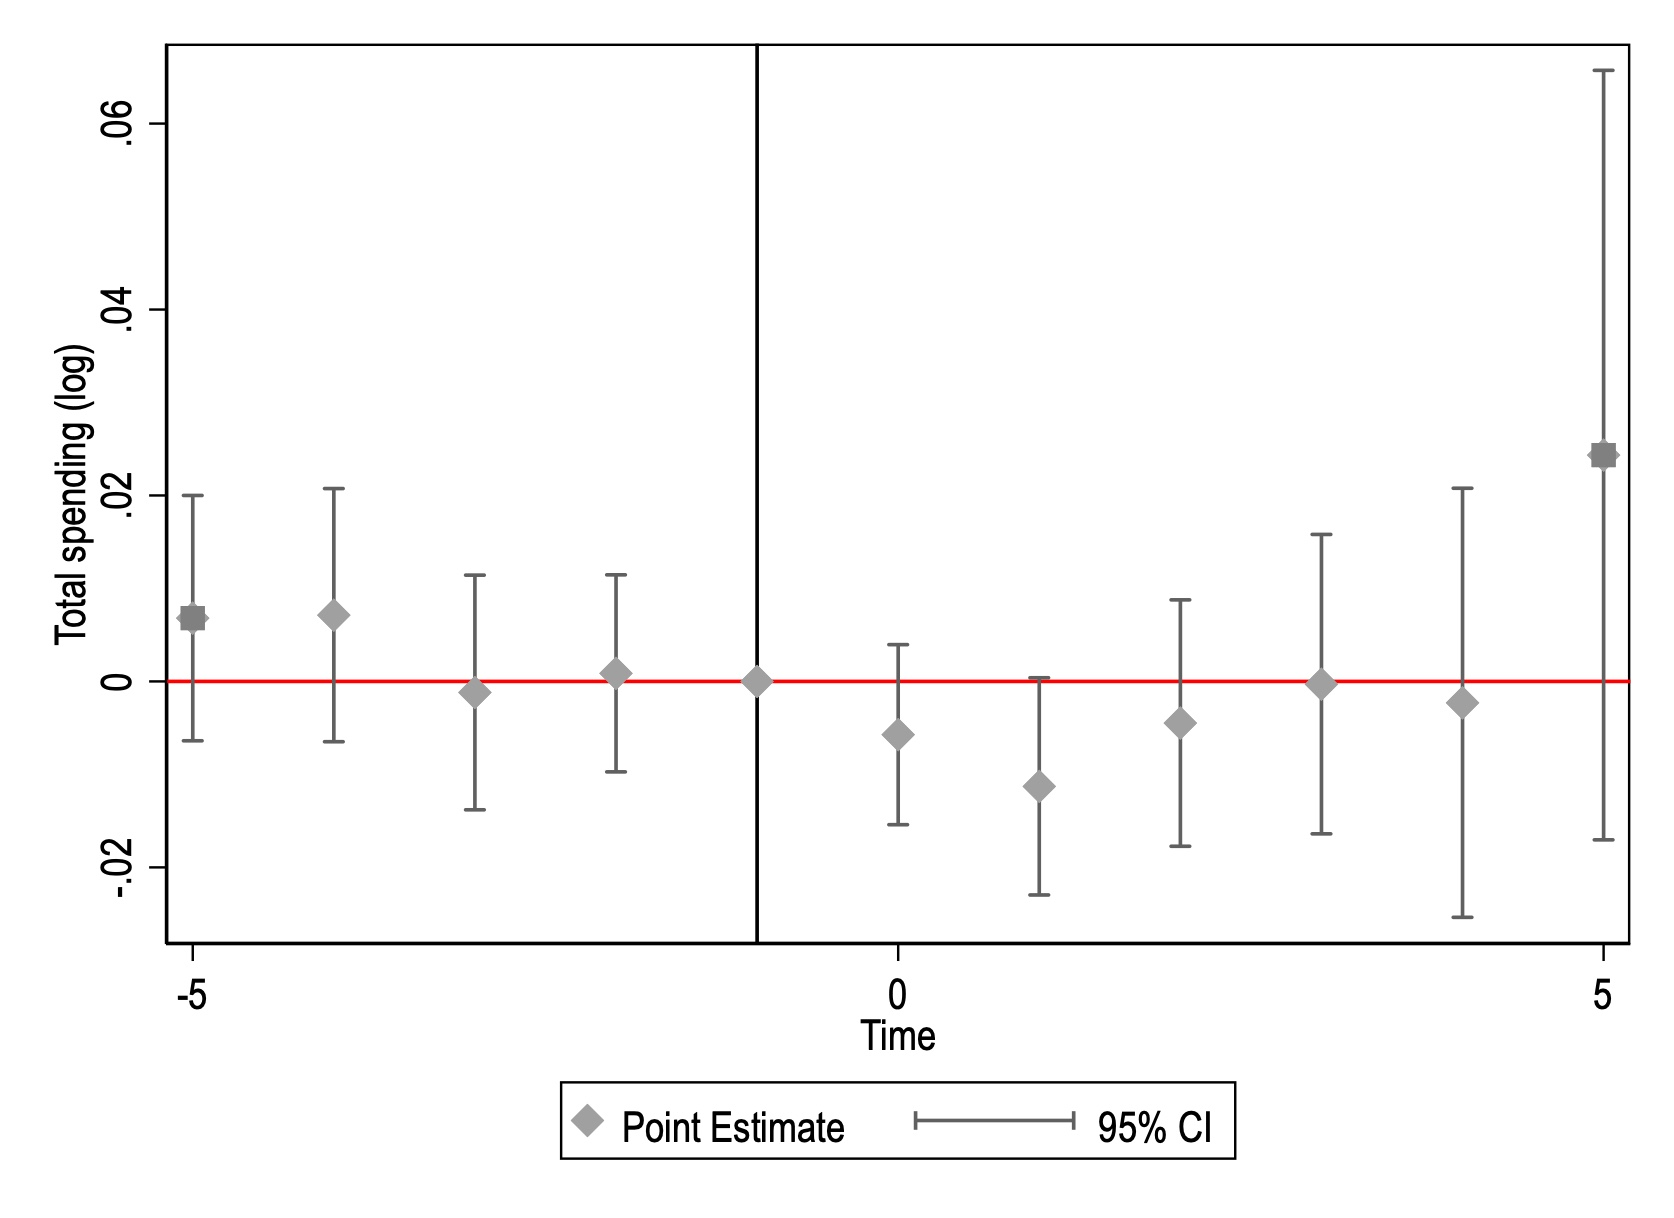
\includegraphics[width=\linewidth]{images/pop_100000/eventdd_ln_q4tot_step1.jpg}
            \label{fig:total_spending}
        \end{minipage} &
        \begin{minipage}[t]{0.32\textwidth}
            \centering
            \caption{Sport}
            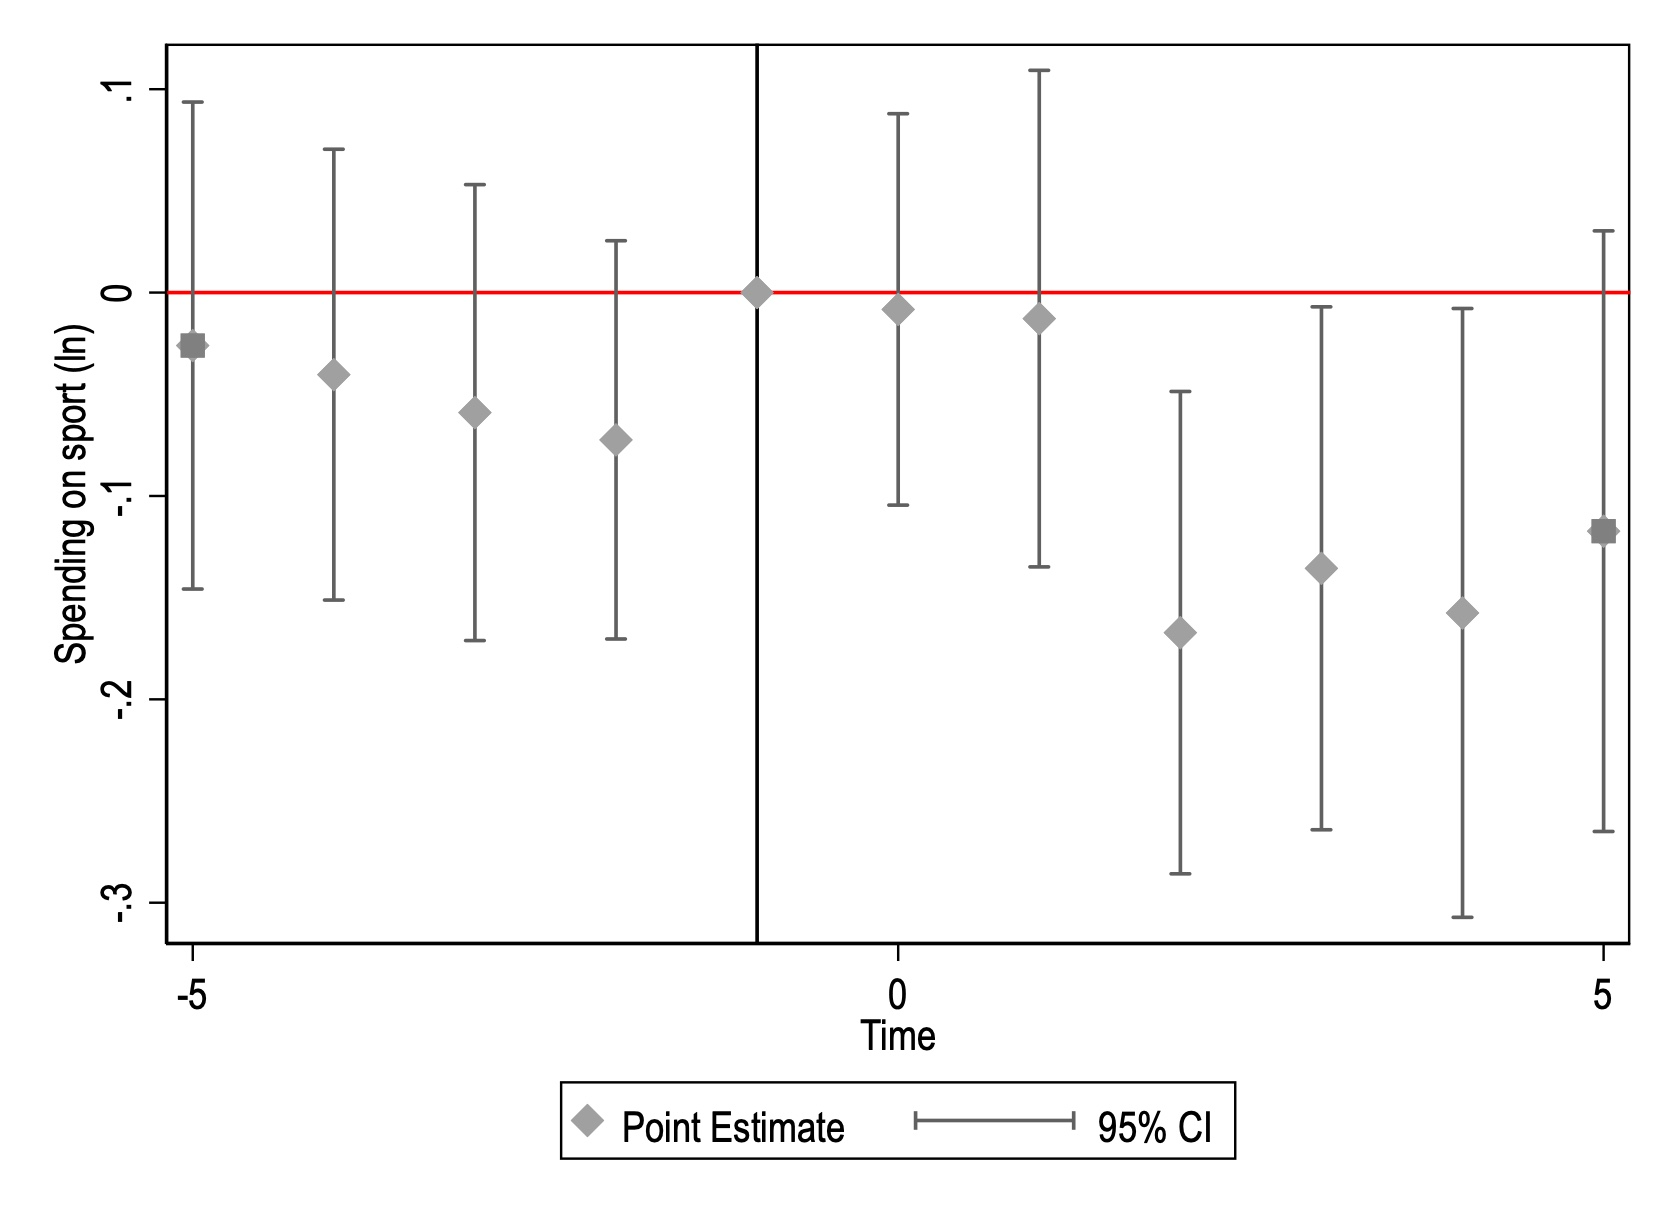
\includegraphics[width=\linewidth]{images/pop_100000/eventdd_ln_q4_06_step1.jpg}
            \label{fig:sport}
        \end{minipage} &
        \begin{minipage}[t]{0.32\textwidth}
            \centering
            \caption{Transport}
            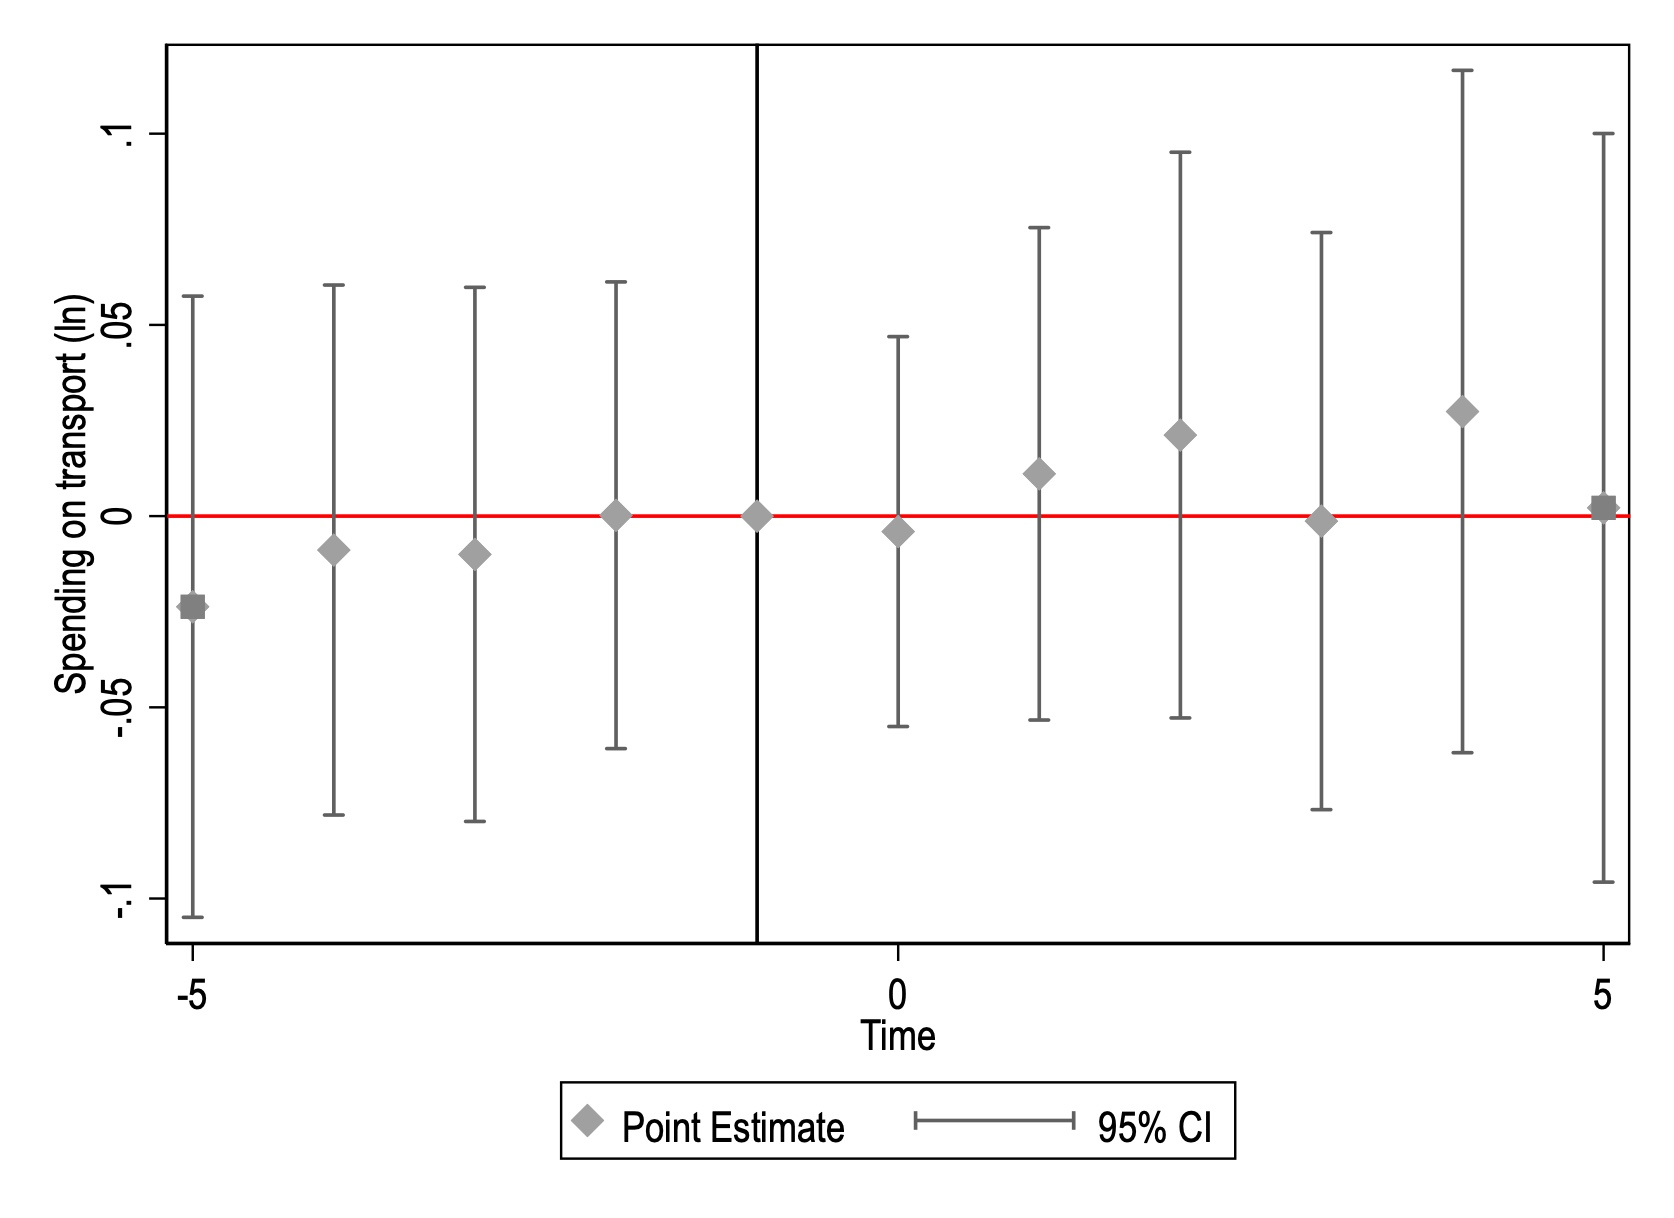
\includegraphics[width=\linewidth]{images/pop_100000/eventdd_ln_q4_08_step1.jpg}
            \label{fig:transport}
        \end{minipage} \\[10pt]

        \begin{minipage}[t]{0.32\textwidth}
            \centering
            \caption{Justice}
            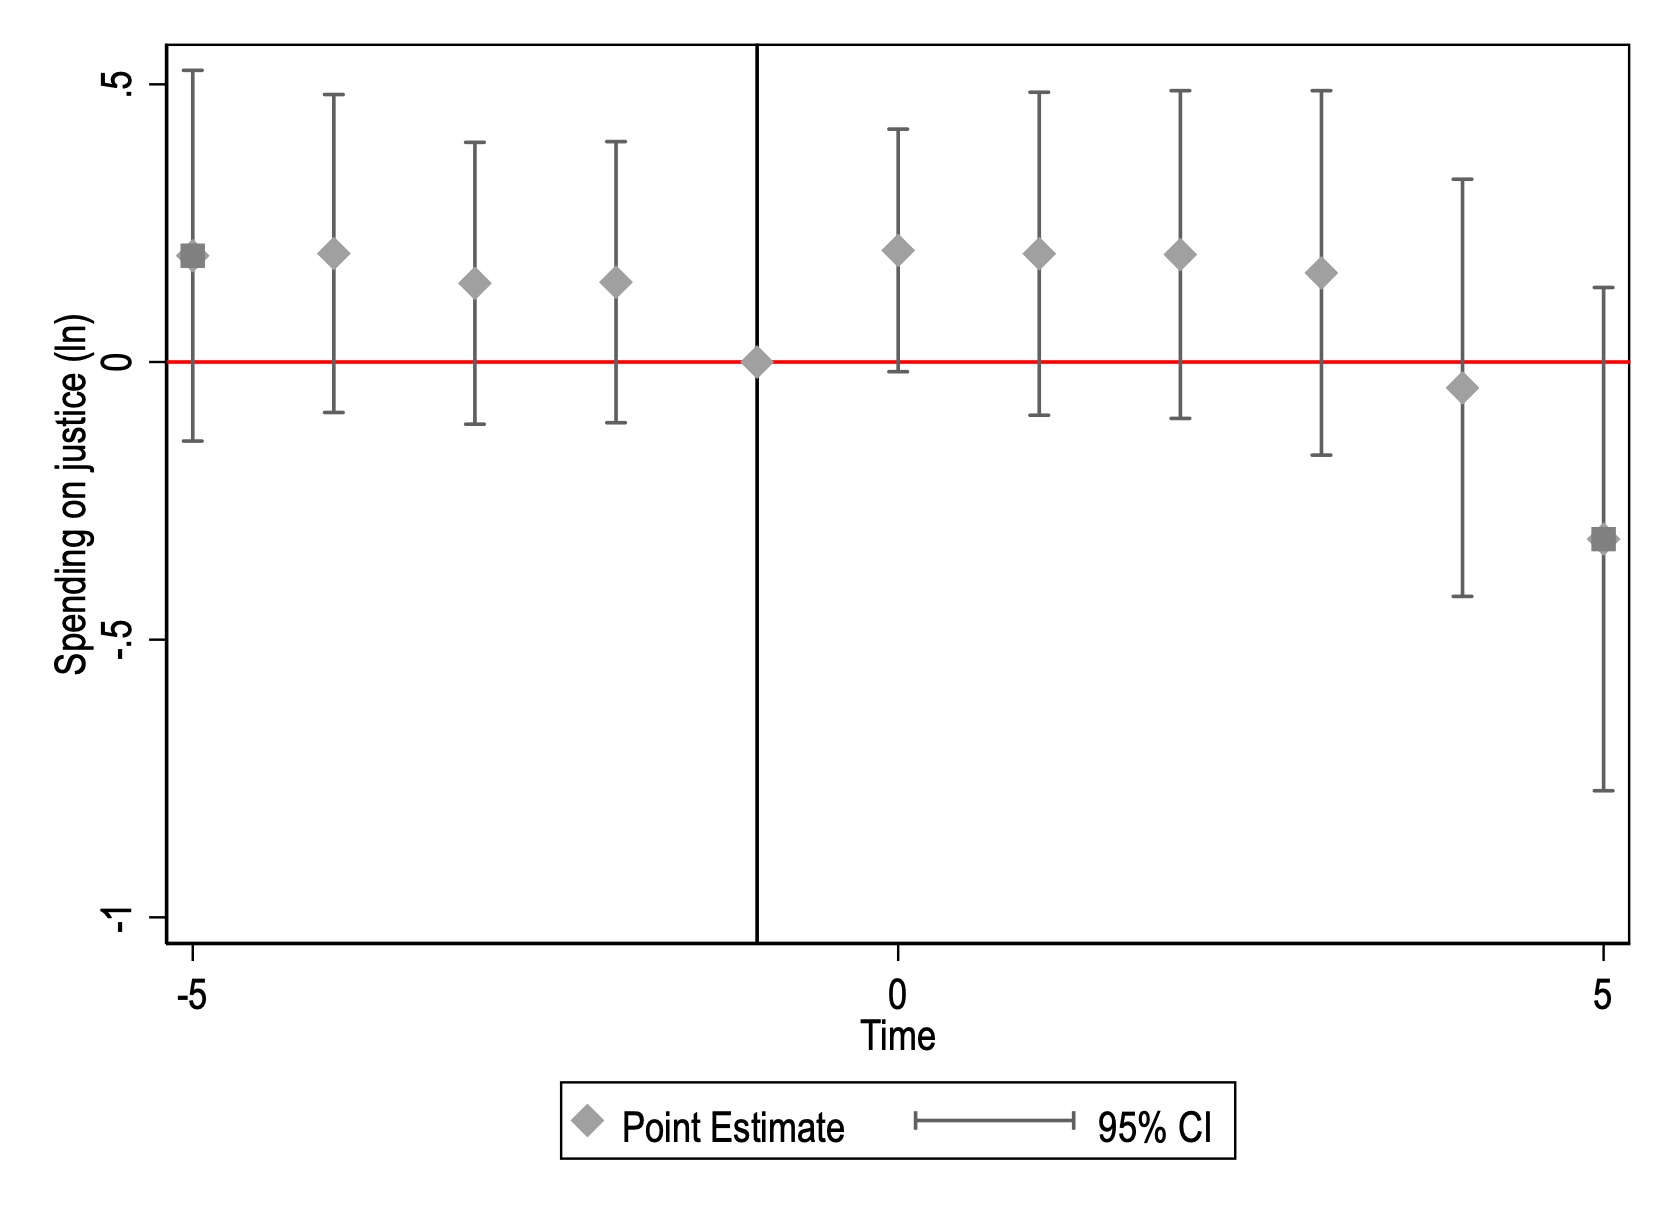
\includegraphics[width=\linewidth]{images/pop_100000/eventdd_ln_q4_02_step1.jpg}
            \label{fig:justice}
        \end{minipage} &
        \begin{minipage}[t]{0.32\textwidth}
            \centering
            \caption{Police}
            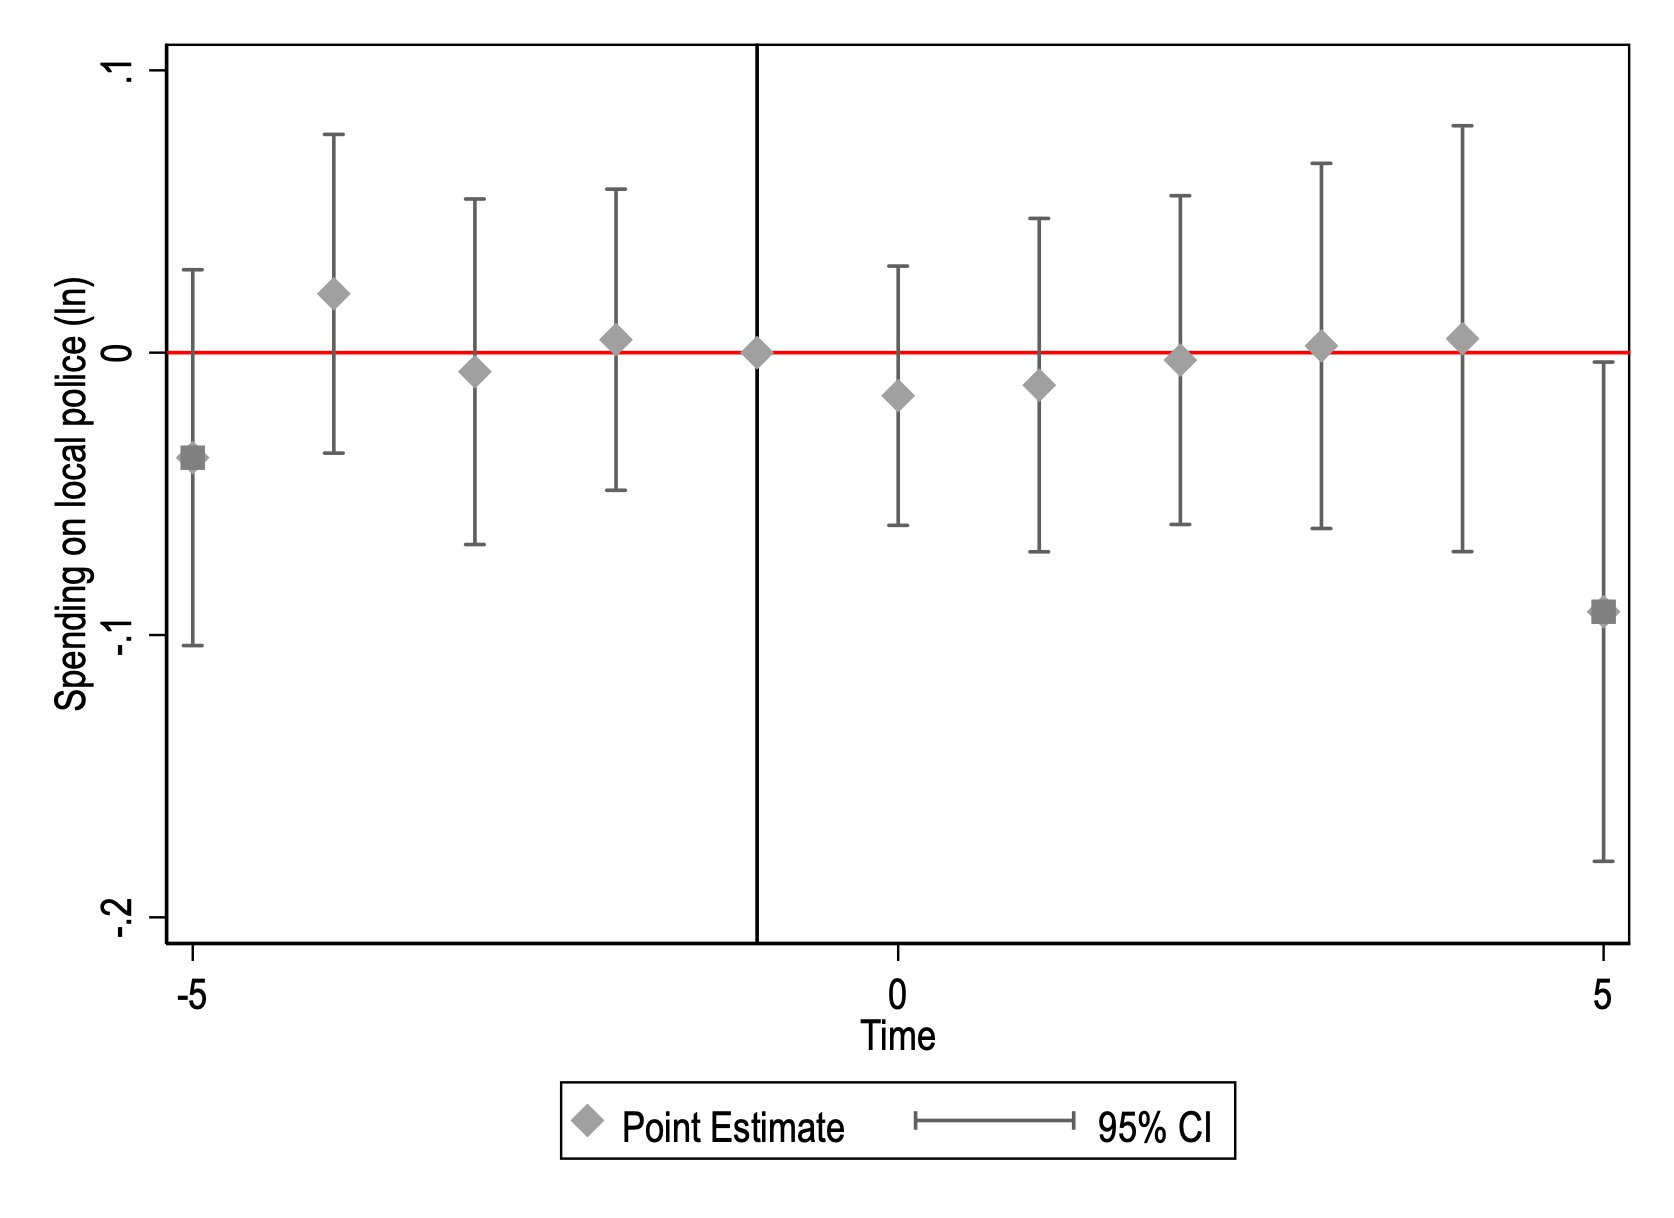
\includegraphics[width=\linewidth]{images/pop_100000/eventdd_ln_q4_03_step1.jpg}
            \label{fig:police}
        \end{minipage} &
        \begin{minipage}[t]{0.32\textwidth}
            \centering
            \caption{Culture, libraries, museums}
            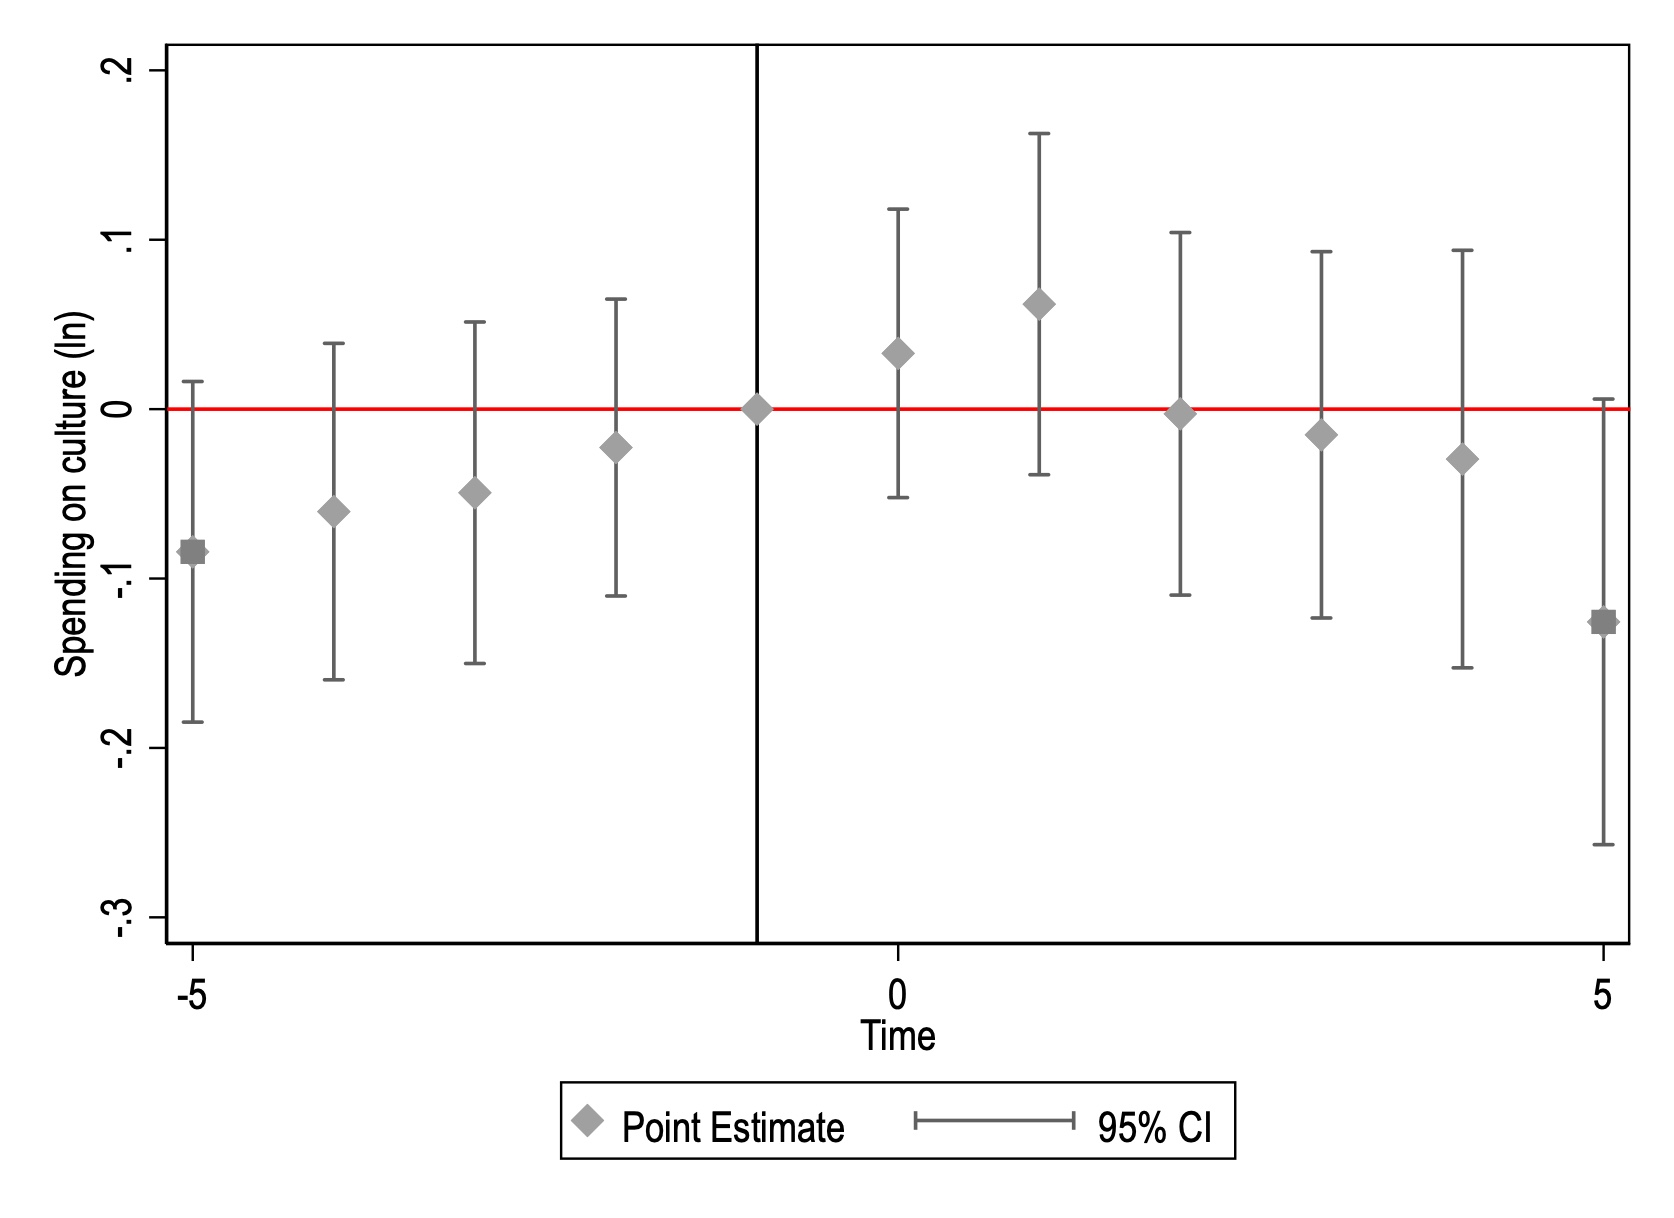
\includegraphics[width=\linewidth]{images/pop_100000/eventdd_ln_q4_05_step1.jpg}
            \label{fig:culture}
        \end{minipage} \\[10pt]

        \begin{minipage}[t]{0.32\textwidth}
            \centering
            \caption{Social services}
            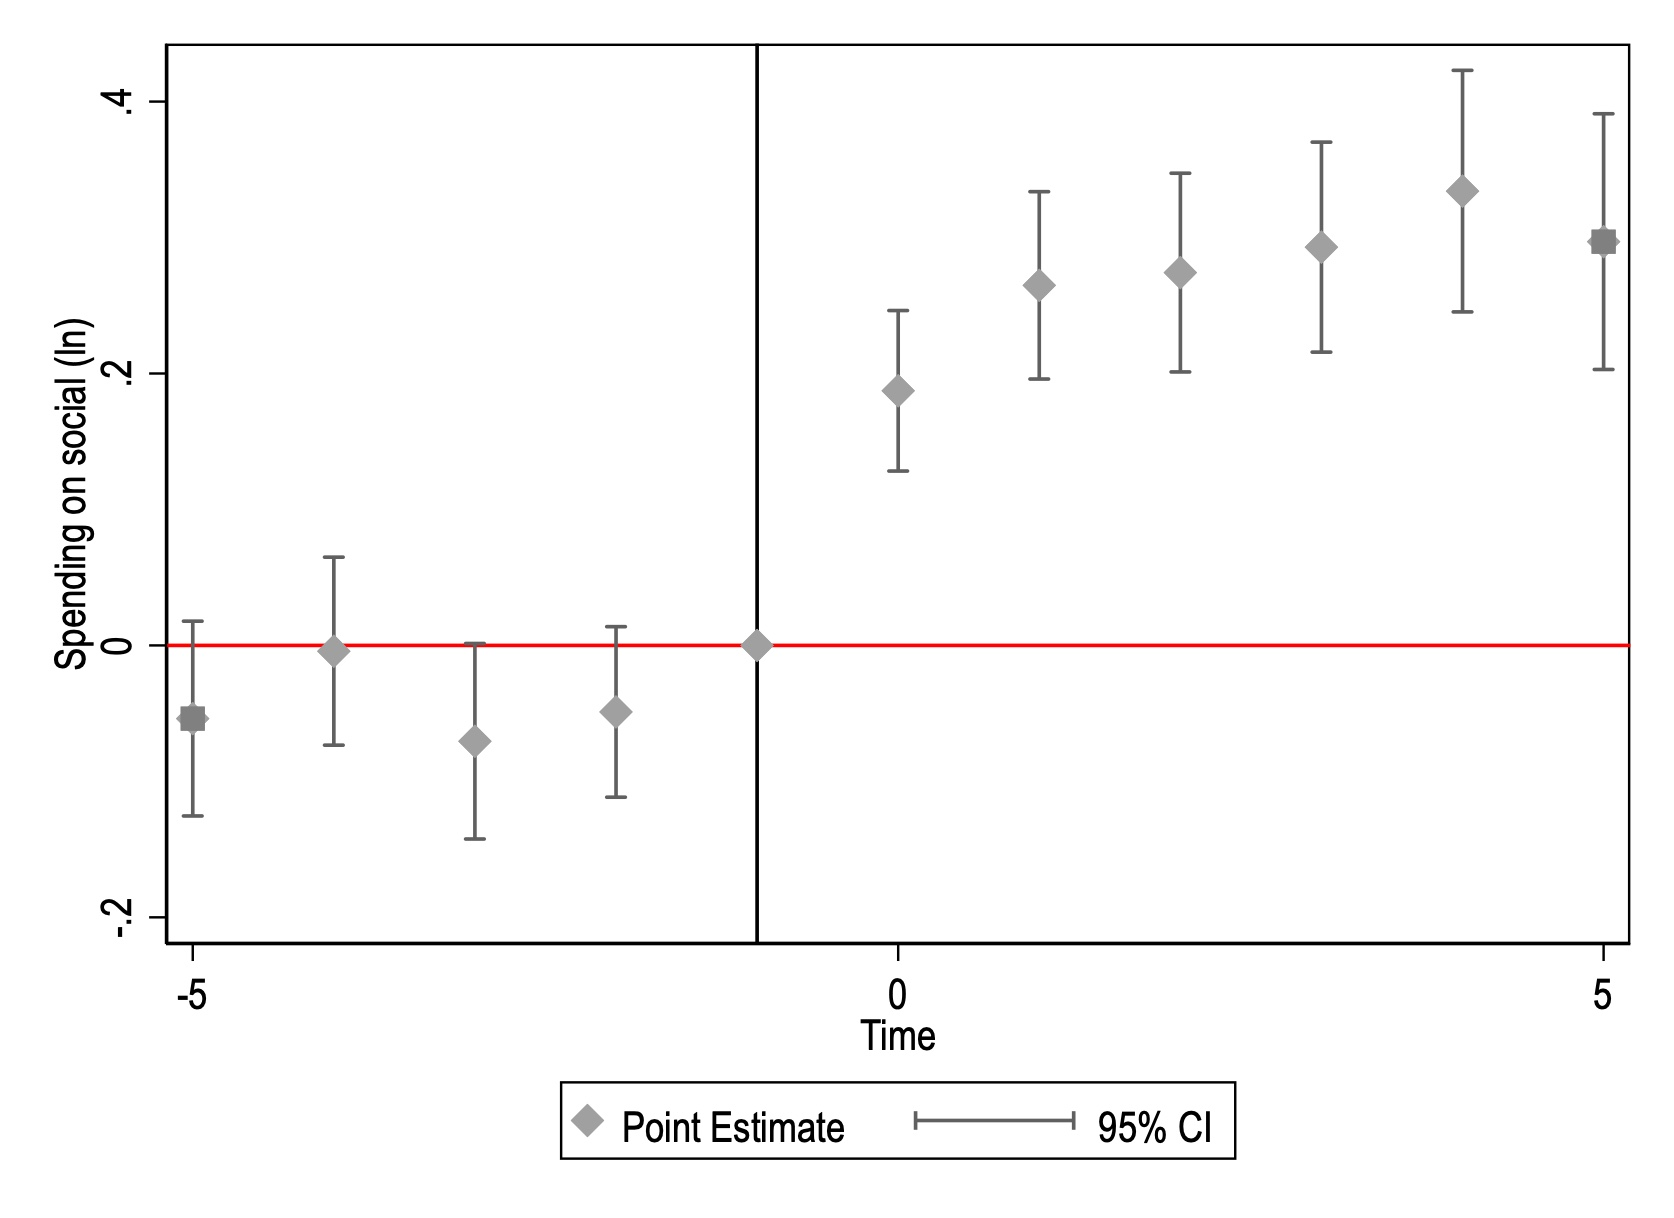
\includegraphics[width=\linewidth]{images/pop_100000/eventdd_ln_q4_10_step1.jpg}
            \label{fig:social_services}
        \end{minipage} &
        \begin{minipage}[t]{0.32\textwidth}
            \centering
            \caption{Education}
            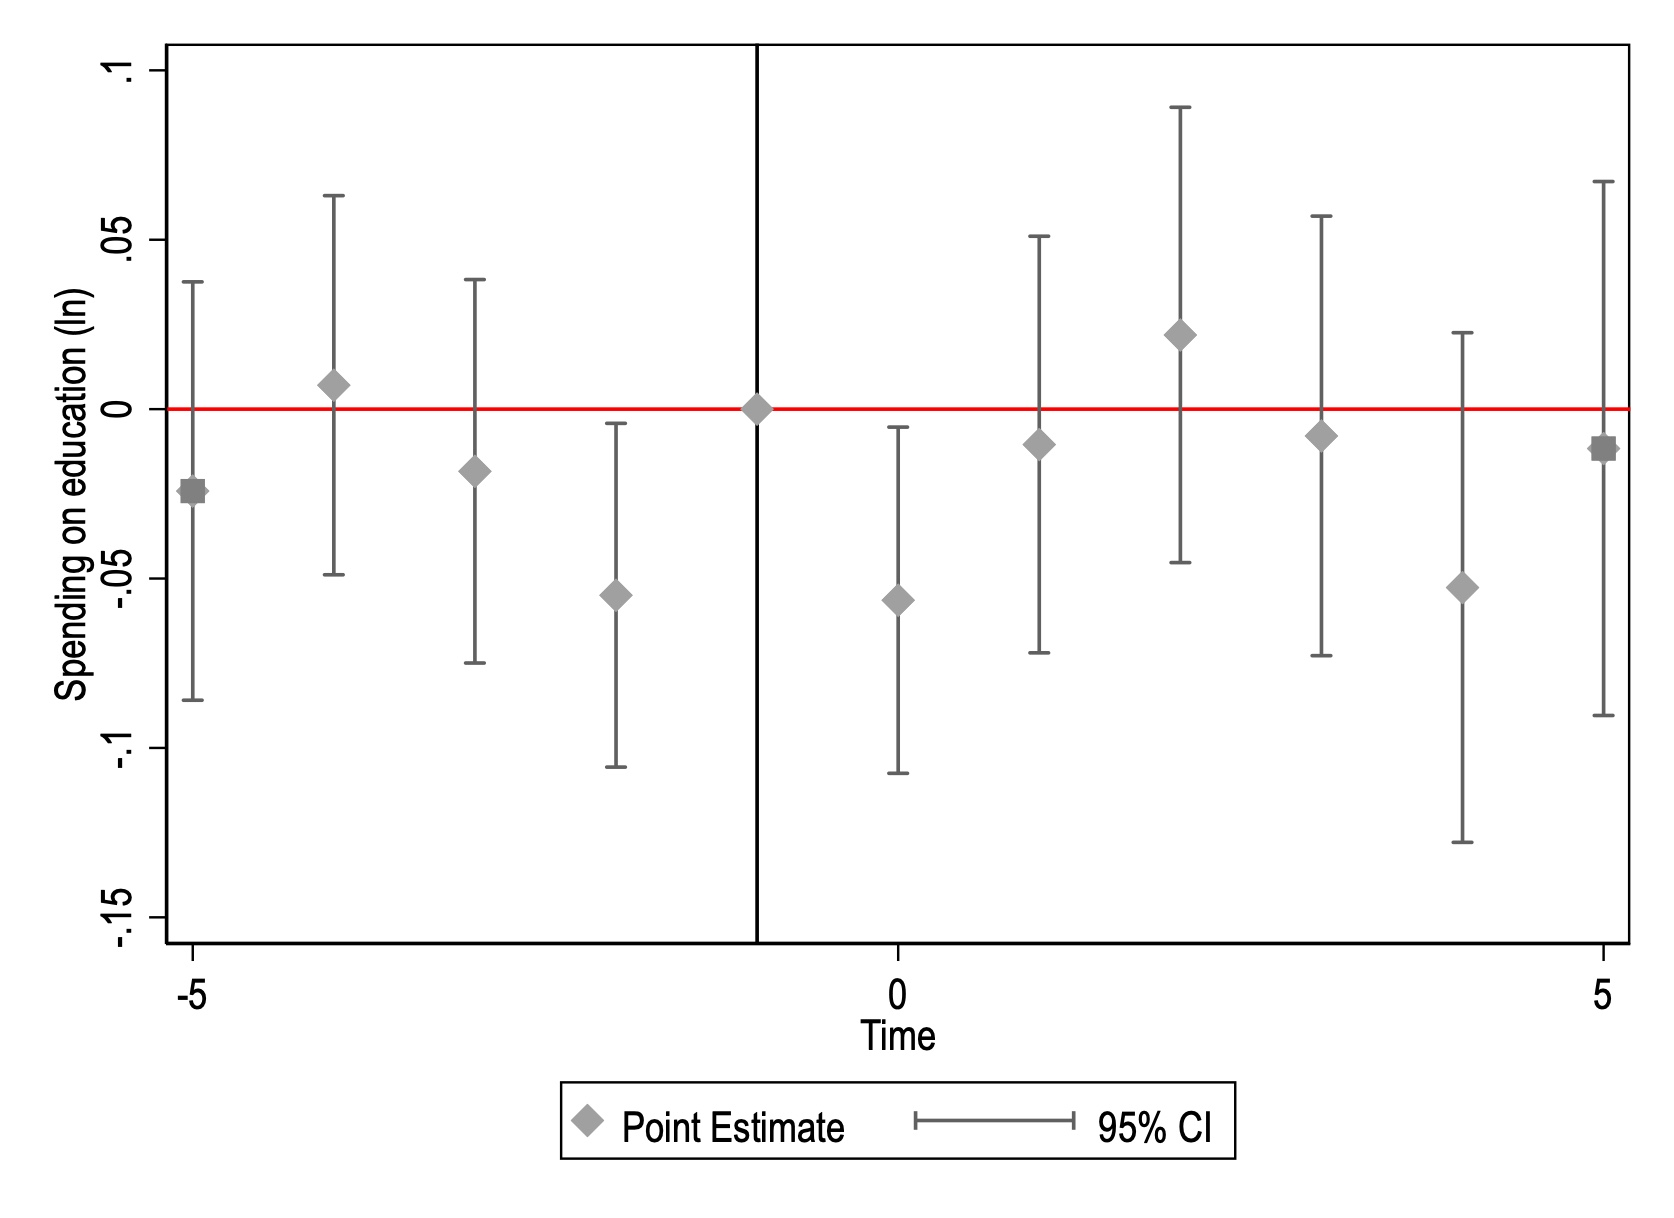
\includegraphics[width=\linewidth]{images/pop_100000/eventdd_ln_q4_04_step1.jpg}
            \label{fig:education}
        \end{minipage} &
        \begin{minipage}[t]{0.32\textwidth}
            \centering
            \caption{Economic development}
            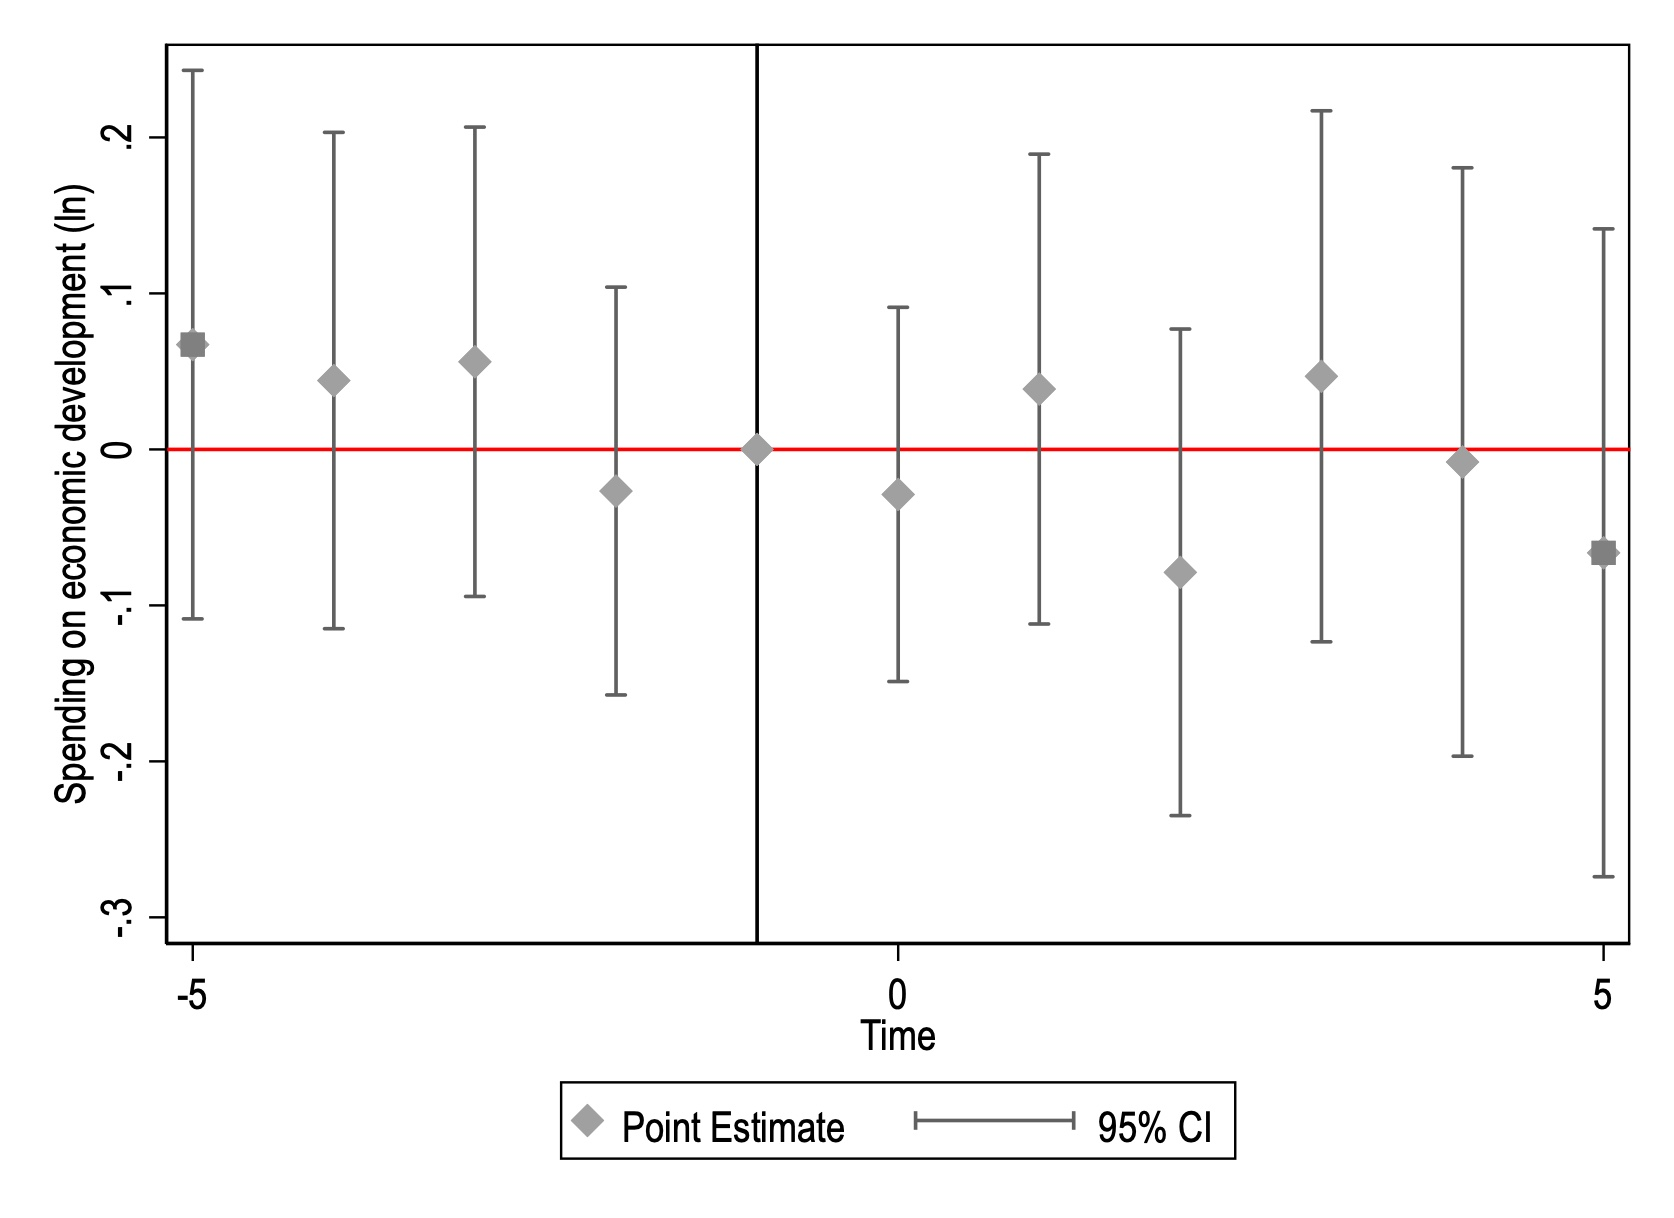
\includegraphics[width=\linewidth]{images/pop_100000/eventdd_ln_q4_11_step1.jpg}
            \label{fig:ecodev}
        \end{minipage} \\[10pt]

        \begin{minipage}[t]{0.32\textwidth}
            \centering
            \caption{Production services}
            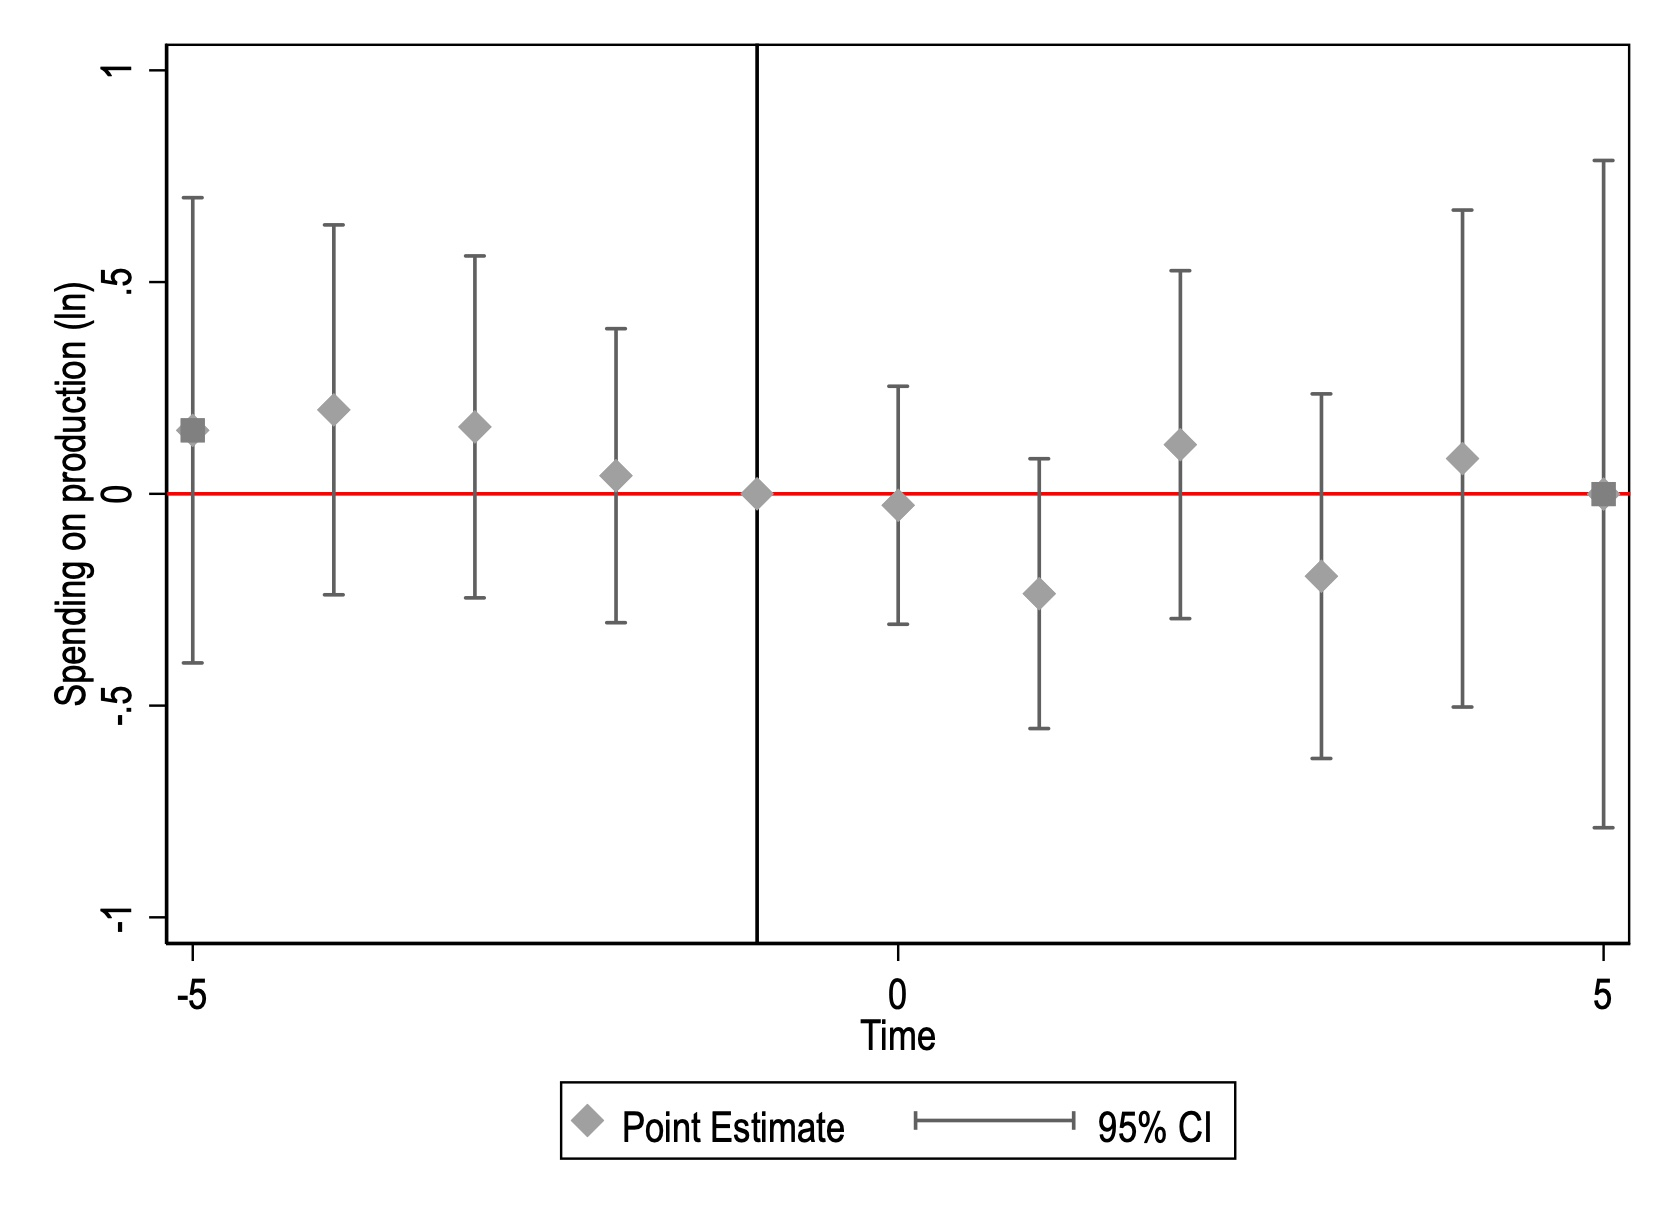
\includegraphics[width=\linewidth]{images/pop_100000/eventdd_ln_q4_12_step1.jpg}
            \label{fig:production}
        \end{minipage} &
        \begin{minipage}[t]{0.32\textwidth}
            \centering
            \caption{Administrative services}
            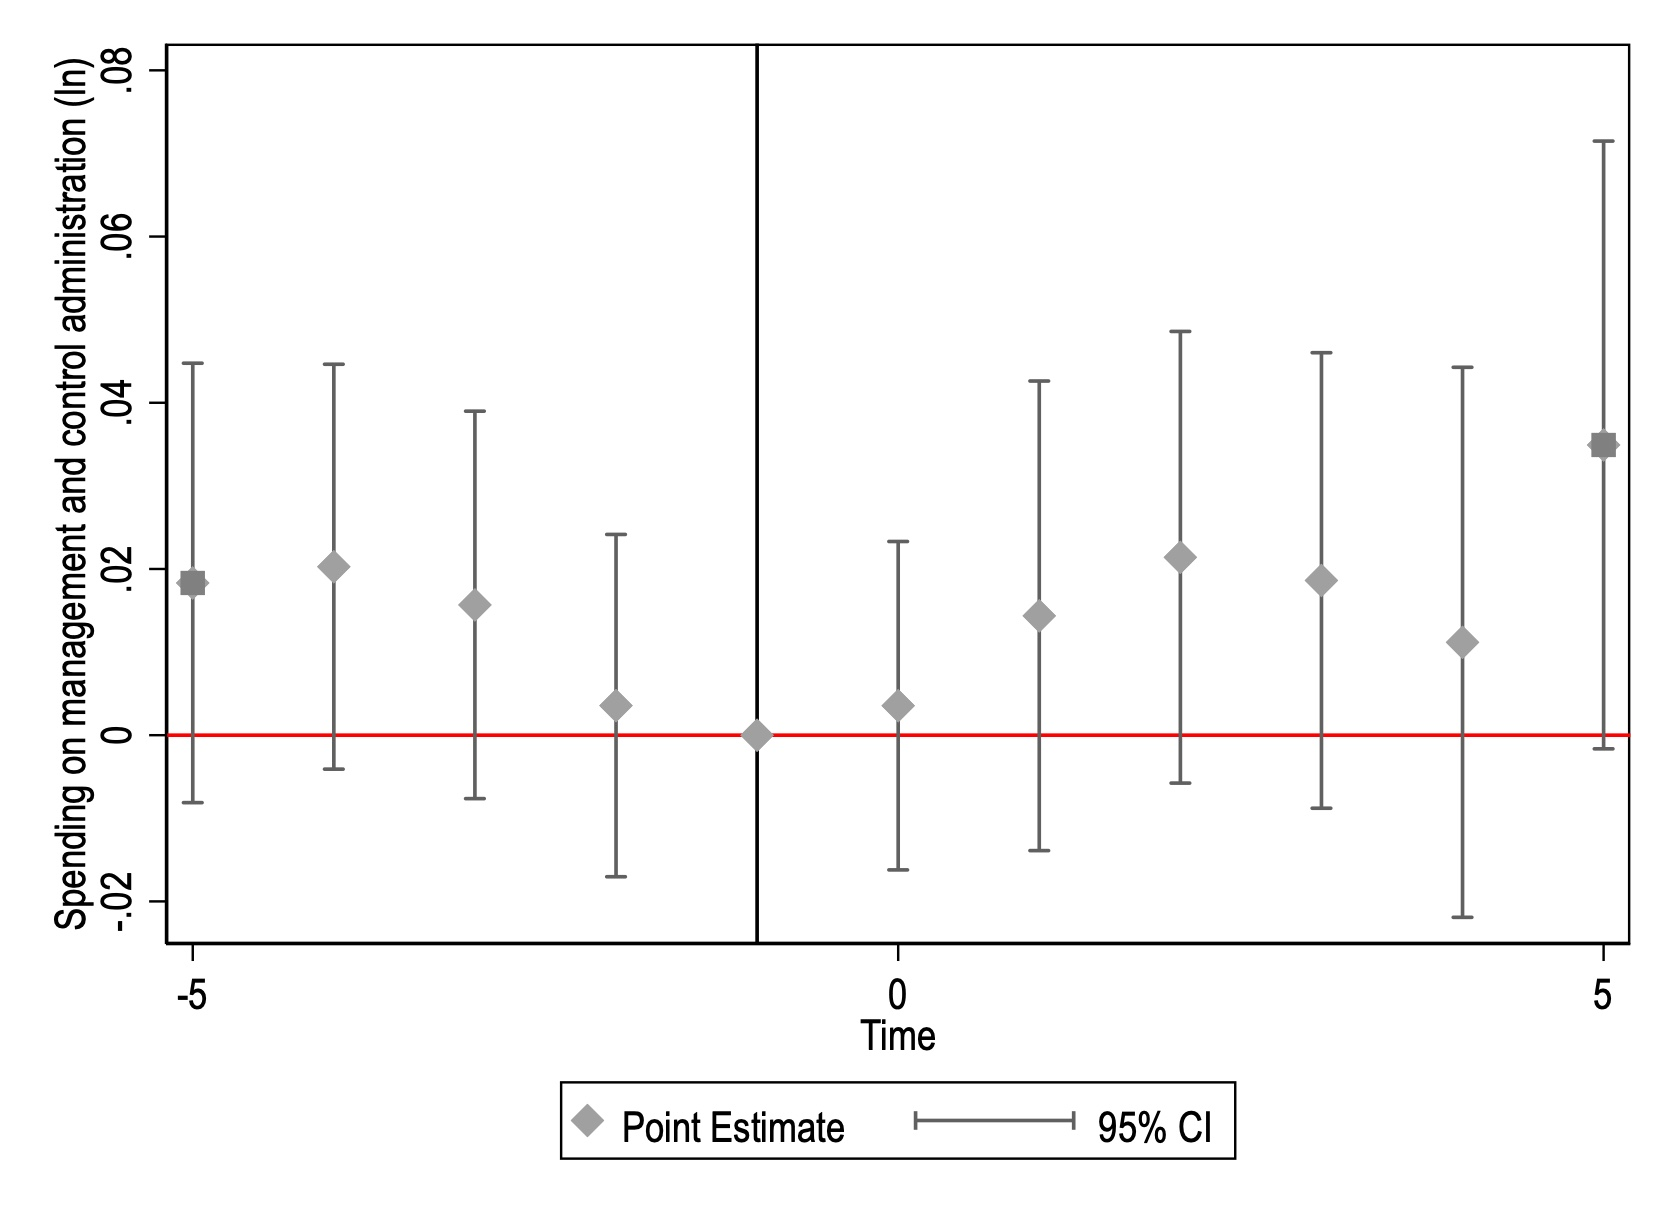
\includegraphics[width=\linewidth]{images/pop_100000/eventdd_ln_q4_01_step1.jpg}
            \label{fig:administration}
        \end{minipage} &
        \begin{minipage}[t]{0.32\textwidth}
            \centering
            \caption{Environment, public parks, recycling}
            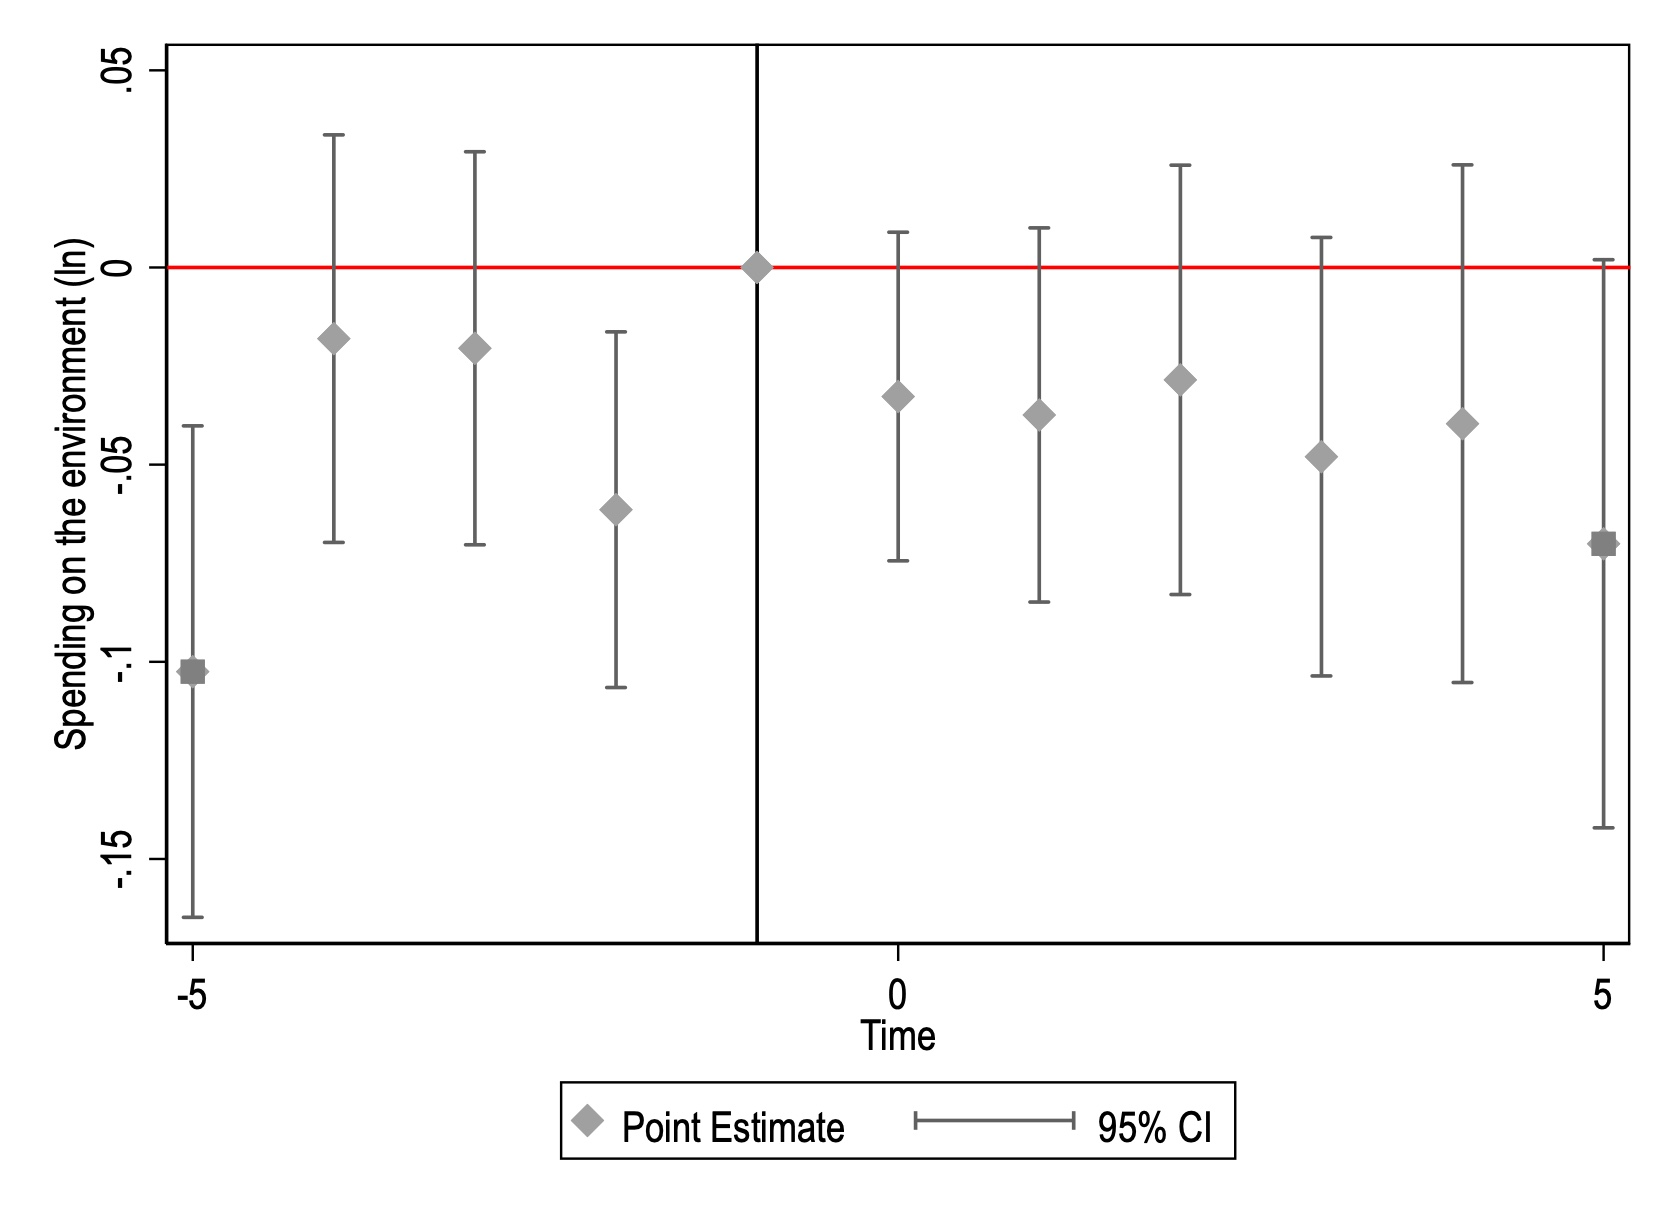
\includegraphics[width=\linewidth]{images/pop_100000/eventdd_ln_q4_09_step1.jpg}
            \label{fig:environment}
        \end{minipage}
    \end{tabular}
\end{figure}



\FloatBarrier

\subsection*{Effects of ASRC on mayor's election}
\normalsize

As a second step, we explore the impact of these types of centers on the local election.\ Following previous literature on the matter \citep{ambrosini2021}, we believe that the impact of the centers on the local community may be relevant also to the politics of the city.\ We run a staggered difference-in-difference with time and municipality fixed-effects to analyse to what extent the opening of a refugee center (either SAI or CAS) in the previous term can affect the outcome of the election.\ We control for municipalities' features in the previous two years (tax and non-tax based revenues, community's tax-base, population, political orientation).\ We differentiate between municipalities that opened the center anytime before the election (columns 1-3), two years before the election (columns 4-6), and only one year before (columns 7-9).\ Results for SAI are shown in Table 1, while Table 2 shows results for CAS centers.\ SAI centers seems to have negative but non-significant effects on mayor's change.\ Namely, the opening of a SAI center does not seem to increase the likelihood of changing the local mayor.\ Conversely, for what concerns CAS centers, the opening of this type of center significantly increases the chances of changing the current mayor.\ Results are robust without restricting the sample (column 1), when using a PSM approach (column 2) and when controlling for municipalities' covariates (column 3).\ We believe that the non-integration feature of the emergency centers, compared to the integration-oriented ones, can have significant and relevant impacts, not only to the local finances, but also to the local elections.\\  

\begin{table}[!ht]
\fontsize{2}{7.2}\selectfont
\renewcommand{\arraystretch}{1.5}
\caption{Regression table for DID analysis on mayor's change - SAI}
\centering

{
\def\sym#1{\ifmmode^{#1}\else\(^{#1}\)\fi}
\begin{tabular}{p{2cm}*{9}{>{\centering\arraybackslash}p{1cm}}}
\hline\hline
                &\multicolumn{1}{c}{(1)}&\multicolumn{1}{c}{(2)}&\multicolumn{1}{c}{(3)}&\multicolumn{1}{c}{(4)}&\multicolumn{1}{c}{(5)}&\multicolumn{1}{c}{(6)}&\multicolumn{1}{c}{(7)}&\multicolumn{1}{c}{(8)}&\multicolumn{1}{c}{(9)}\\
                &\multicolumn{1}{c}{MC}&\multicolumn{1}{c}{MC}&\multicolumn{1}{c}{MC}&\multicolumn{1}{c}{MC}&\multicolumn{1}{c}{MC}&\multicolumn{1}{c}{MC}&\multicolumn{1}{c}{MC}&\multicolumn{1}{c}{MC}&\multicolumn{1}{c}{MC}\\
\hline
SAI opening (anytime previous term)& -0.00159         &  -0.0116         &  -0.0334         &                  &                  &                  &                  &                  &                  \\
                &  (-0.09)         &  (-0.65)         &  (-1.44)         &                  &                  &                  &                  &                  &                  \\
[1em]
SAI opening (within two years before)&                  &                  &                  &  -0.0203         &  -0.0187         &  -0.0311         &                  &                  &                  \\
                &                  &                  &                  &  (-0.98)         &  (-0.88)         &  (-1.17)         &                  &                  &                  \\
[1em]
SAI opening (within previous year)&                  &                  &                  &                  &                  &                  &  -0.0194         &  -0.0171         &  -0.0268         \\
                &                  &                  &                  &                  &                  &                  &  (-0.45)         &  (-0.40)         &  (-0.53)         \\
[1em]
CAS center      &   0.0336\sym{*}  &   0.0288\sym{*}  &   0.0161         &   0.0328\sym{*}  &   0.0300\sym{*}  &   0.0217         &   0.0304\sym{*}  &   0.0285         &   0.0138         \\
                &   (2.53)         &   (2.07)         &   (0.57)         &   (2.38)         &   (2.08)         &   (0.68)         &   (2.07)         &   (1.85)         &   (0.32)         \\
[1em]
Municipality's covariates (year - 1) &       No         &      Yes         &      Yes         &       No         &      Yes         &      Yes         &       No         &      Yes         &      Yes         \\
[1em]
Municipality's covariates (year - 2) &       No         &      Yes         &      Yes         &       No         &      Yes         &      Yes         &       No         &      Yes         &      Yes         \\
\hline
N               &    29100         &    27223         &     6038         &    26946         &    25431         &     4535         &    25302         &    23797         &     3158         \\
Municipality FE &      Yes         &      Yes         &      Yes         &      Yes         &      Yes         &      Yes         &      Yes         &      Yes         &      Yes         \\
Year FE         &      Yes         &      Yes         &      Yes         &      Yes         &      Yes         &      Yes         &      Yes         &      Yes         &      Yes         \\
Adjusted-R squared&    0.382         &    0.381         &    0.399         &    0.391         &    0.391         &    0.444         &    0.383         &    0.381         &    0.419         \\
\hline\hline


\multicolumn{10}{l}{\tiny \textit{t} statistics in parentheses}\\
\multicolumn{10}{l}{\tiny \sym{*} \(p<0.10\), \sym{**} \(p<0.05\), \sym{***} \(p<0.01\)}\\
\end{tabular}
}
\end{table}

\begin{table}[!ht]
\fontsize{2}{7.2}\selectfont
\renewcommand{\arraystretch}{1.5}
\caption{Regression table for DID analysis on mayor's change - CAS}
\centering
{
\def\sym#1{\ifmmode^{#1}\else\(^{#1}\)\fi}
\begin{tabular}{p{2cm}*{9}{>{\centering\arraybackslash}p{1cm}}}
\hline\hline
                &\multicolumn{1}{c}{(1)}&\multicolumn{1}{c}{(2)}&\multicolumn{1}{c}{(3)}&\multicolumn{1}{c}{(4)}&\multicolumn{1}{c}{(5)}&\multicolumn{1}{c}{(6)}&\multicolumn{1}{c}{(7)}&\multicolumn{1}{c}{(8)}&\multicolumn{1}{c}{(9)}\\
                &\multicolumn{1}{c}{MC}&\multicolumn{1}{c}{MC}&\multicolumn{1}{c}{MC}&\multicolumn{1}{c}{MC}&\multicolumn{1}{c}{MC}&\multicolumn{1}{c}{MC}&\multicolumn{1}{c}{MC}&\multicolumn{1}{c}{MC}&\multicolumn{1}{c}{MC}\\
\hline
CAS opening (anytime previous term)&   0.0366\sym{*}  &   0.0350\sym{*}  &   0.0475\sym{**} &                  &                  &                  &                  &                  &                  \\
                &   (2.47)         &   (2.25)         &   (2.74)         &                  &                  &                  &                  &                  &                  \\
[1em]
CAS opening (within two years before)&                  &                  &                  &   0.0348\sym{*}  &   0.0324\sym{*}  &   0.0386\sym{*}  &                  &                  &                  \\
                &                  &                  &                  &   (2.37)         &   (2.12)         &   (2.31)         &                  &                  &                  \\
[1em]
CAS opening (within previous year)&                  &                  &                  &                  &                  &                  &   0.0176         &   0.0107         &   0.0140         \\
                &                  &                  &                  &                  &                  &                  &   (0.94)         &   (0.56)         &   (0.68)         \\
[1em]
SAI center      & -0.00595         &  -0.0237         &   0.0120         &  -0.0181         &  -0.0232         &   0.0194         & -0.00366         &  -0.0116         &   0.0406         \\
                &  (-0.33)         &  (-1.24)         &   (0.53)         &  (-0.97)         &  (-1.20)         &   (0.84)         &  (-0.18)         &  (-0.56)         &   (1.61)         \\
[1em]
Municipality's covariates (year - 1) &       No         &      Yes         &      Yes         &       No         &      Yes         &      Yes         &       No         &      Yes         &      Yes         \\
[1em]
Municipality's covariates (year - 2) &       No         &      Yes         &      Yes         &       No         &      Yes         &      Yes         &       No         &      Yes         &      Yes         \\
\hline
N               &    24795         &    23237         &    14545         &    27647         &    25944         &    17130         &    26735         &    25027         &    16277         \\
Municipality FE &      Yes         &      Yes         &      Yes         &      Yes         &      Yes         &      Yes         &      Yes         &      Yes         &      Yes         \\
Year FE         &      Yes         &      Yes         &      Yes         &      Yes         &      Yes         &      Yes         &      Yes         &      Yes         &      Yes         \\
Adjusted-R squared&    0.406         &    0.407         &    0.415         &    0.392         &    0.391         &    0.390         &    0.396         &    0.396         &    0.398         \\
\hline\hline

\multicolumn{10}{l}{\tiny \textit{t} statistics in parentheses}\\
\multicolumn{10}{l}{\tiny \sym{*} \(p<0.10\), \sym{**} \(p<0.05\), \sym{***} \(p<0.01\)}\\
\end{tabular}
}


\end{table}

\section*{Conclusions}

\normalsize

\noindent
This is the first paper to empirically study the effects of different types of reception facilities for asylum seekers in Italy.\ We focus on municipalities' public finances, controlling for other variables.\ We find a positive and significant effect of SAI centers (multi-level governance and integration-oriented) on social spending and a negative impact on youth and free-time related activties.\ While the spending on social services is more than expected, since the municipality is the owner of the project, the spillovers of other functions may have different implications.\ For what concerns the government-run CAS centers (top-down and not integration-oriented), we see a negative and significant impact on spending related to social activities such as culture, environment, and economic development.\ The same municipalities seem to increase instead expenses related to local police and education.\ These differences in financial patterns may be due to the different perception and levels of integration that these two types of centers have.\ Our conclusion are corrobarated by the second step of our analysis, when we explore the impact on local elections.\ SAI centers have negative although non significant effects on local elections, i.e.\ they do not affect the chances of the mayor to be reelected.\ On the other side, CAS centers have a positive and relevant impact on the outcome of the election.\ Chances to change mayor are higher when a CAS center has been opened in the previous term, compared to non-treated municipalities.\ We believe that our results provide evidence of significant differences between spillovers on local communities of different types of refugee centers, where integration-oriented centers are more likely to have positive effects on local communities compared to non-integration oriented ones.\\ 



\bibliography{references2}

\section{Appendix}



\subsection{Cities with less than 5'000 people}


\justifying
\noindent
Results for smaller municipalities (population \(\leq\) 5'000) \\

\vspace{5}

\input{tables/pop_5000/descriptive stats sai.txt}
\input{tables/pop_5000/descriptive stats cas.txt}

\begin{figure}[ht]
\fontsize{7.2}{7.2}\selectfont
    \centering
\caption*{Effect of SAI centers on municipalities' public spending}
    \begin{tabular}{@{}ccc@{}}
        \begin{minipage}[t]{0.32\textwidth}
            \centering
            \caption{Total spending}
            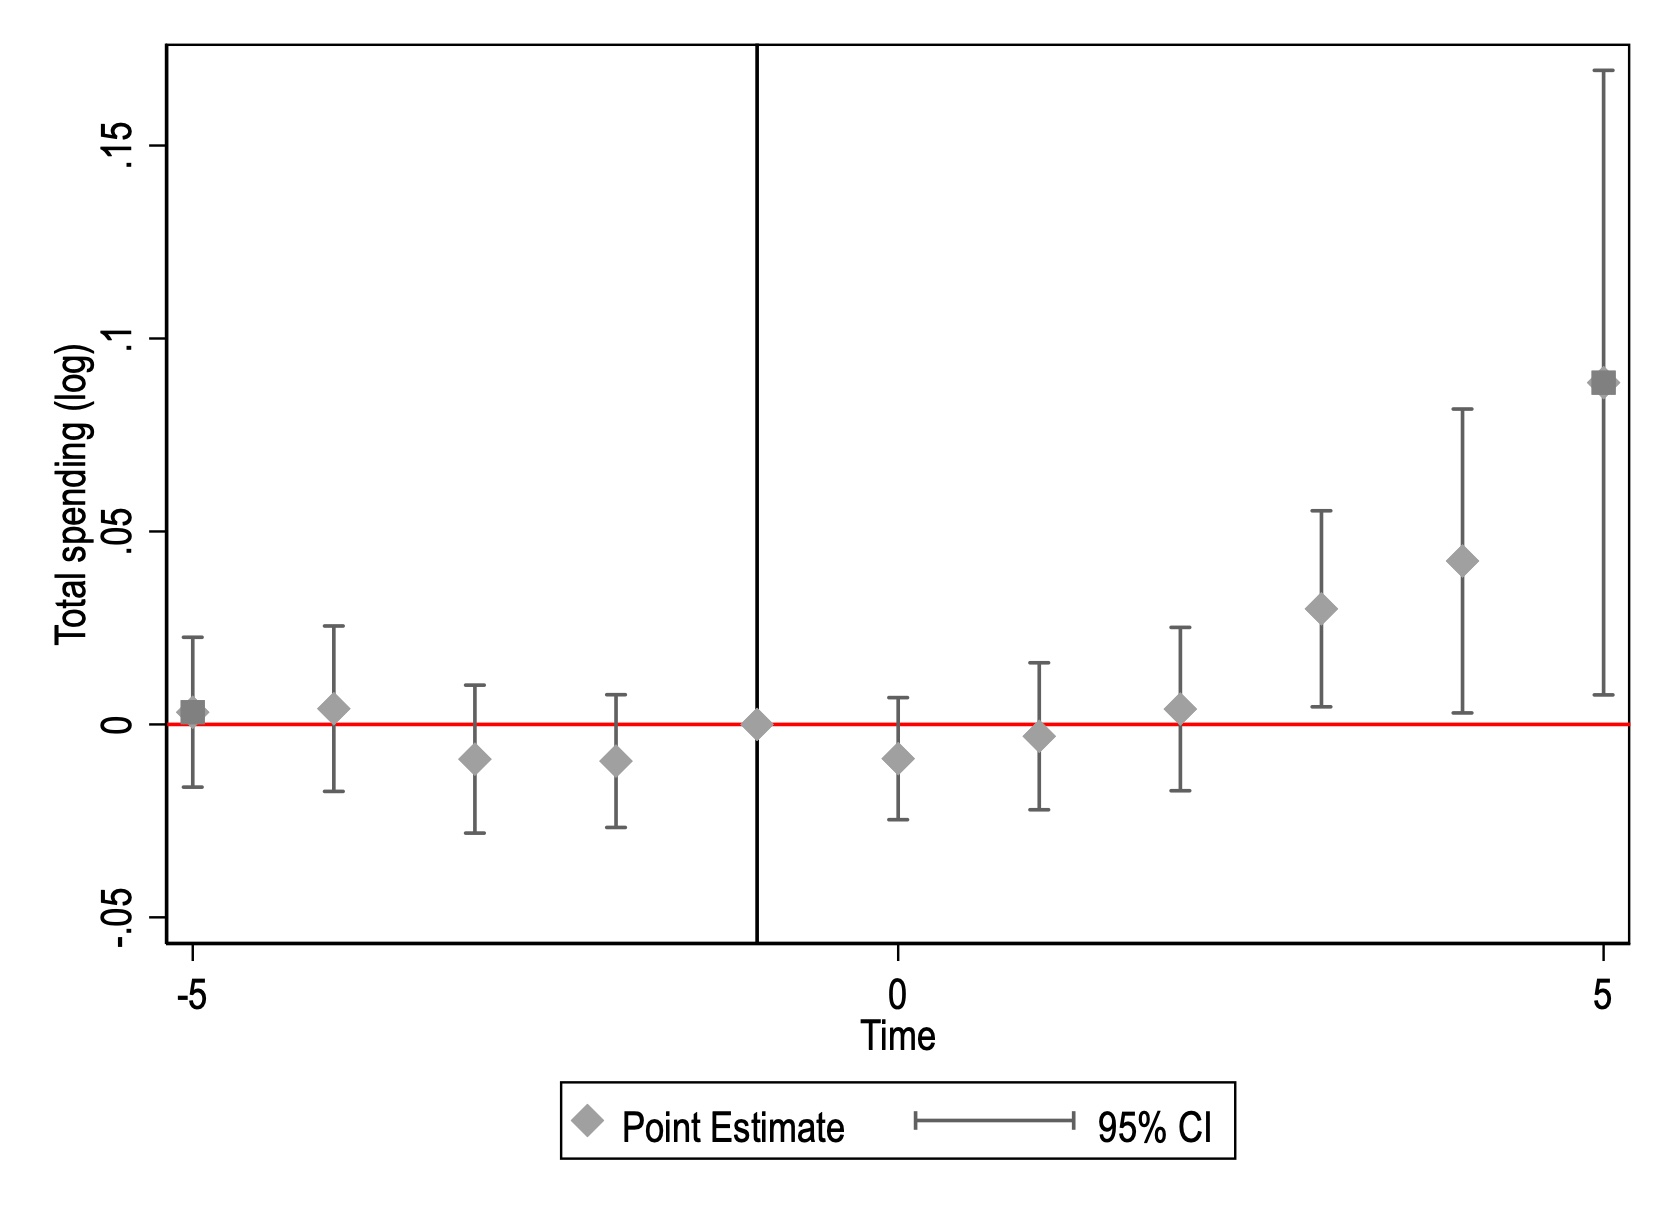
\includegraphics[width=\linewidth]{images/pop_5000/eventdd_ln_q4tot_step1.jpg}
            \label{fig:total_spending}
        \end{minipage} &
        \begin{minipage}[t]{0.32\textwidth}
            \centering
            \caption{Sport}
            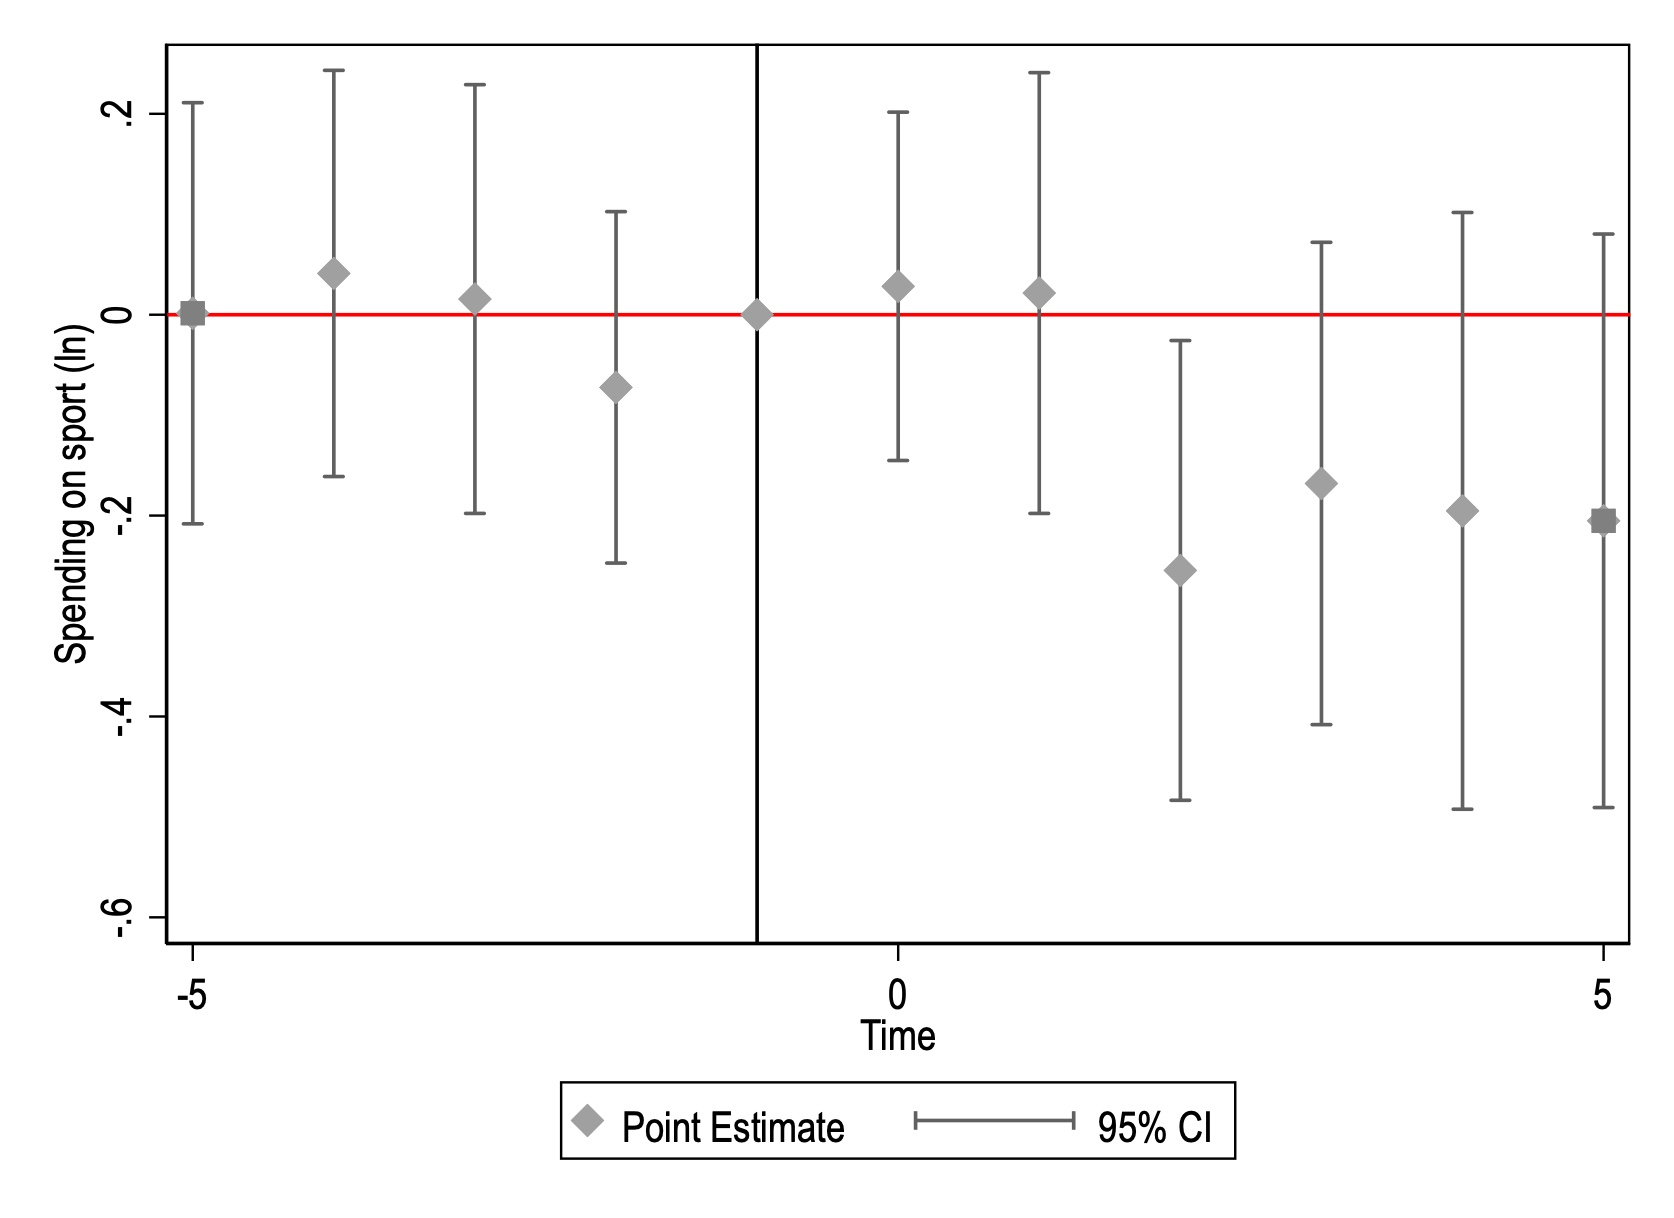
\includegraphics[width=\linewidth]{images/pop_5000/eventdd_ln_q4_06_step1.jpg}
            \label{fig:sport}
        \end{minipage} &
        \begin{minipage}[t]{0.32\textwidth}
            \centering
            \caption{Transport}
            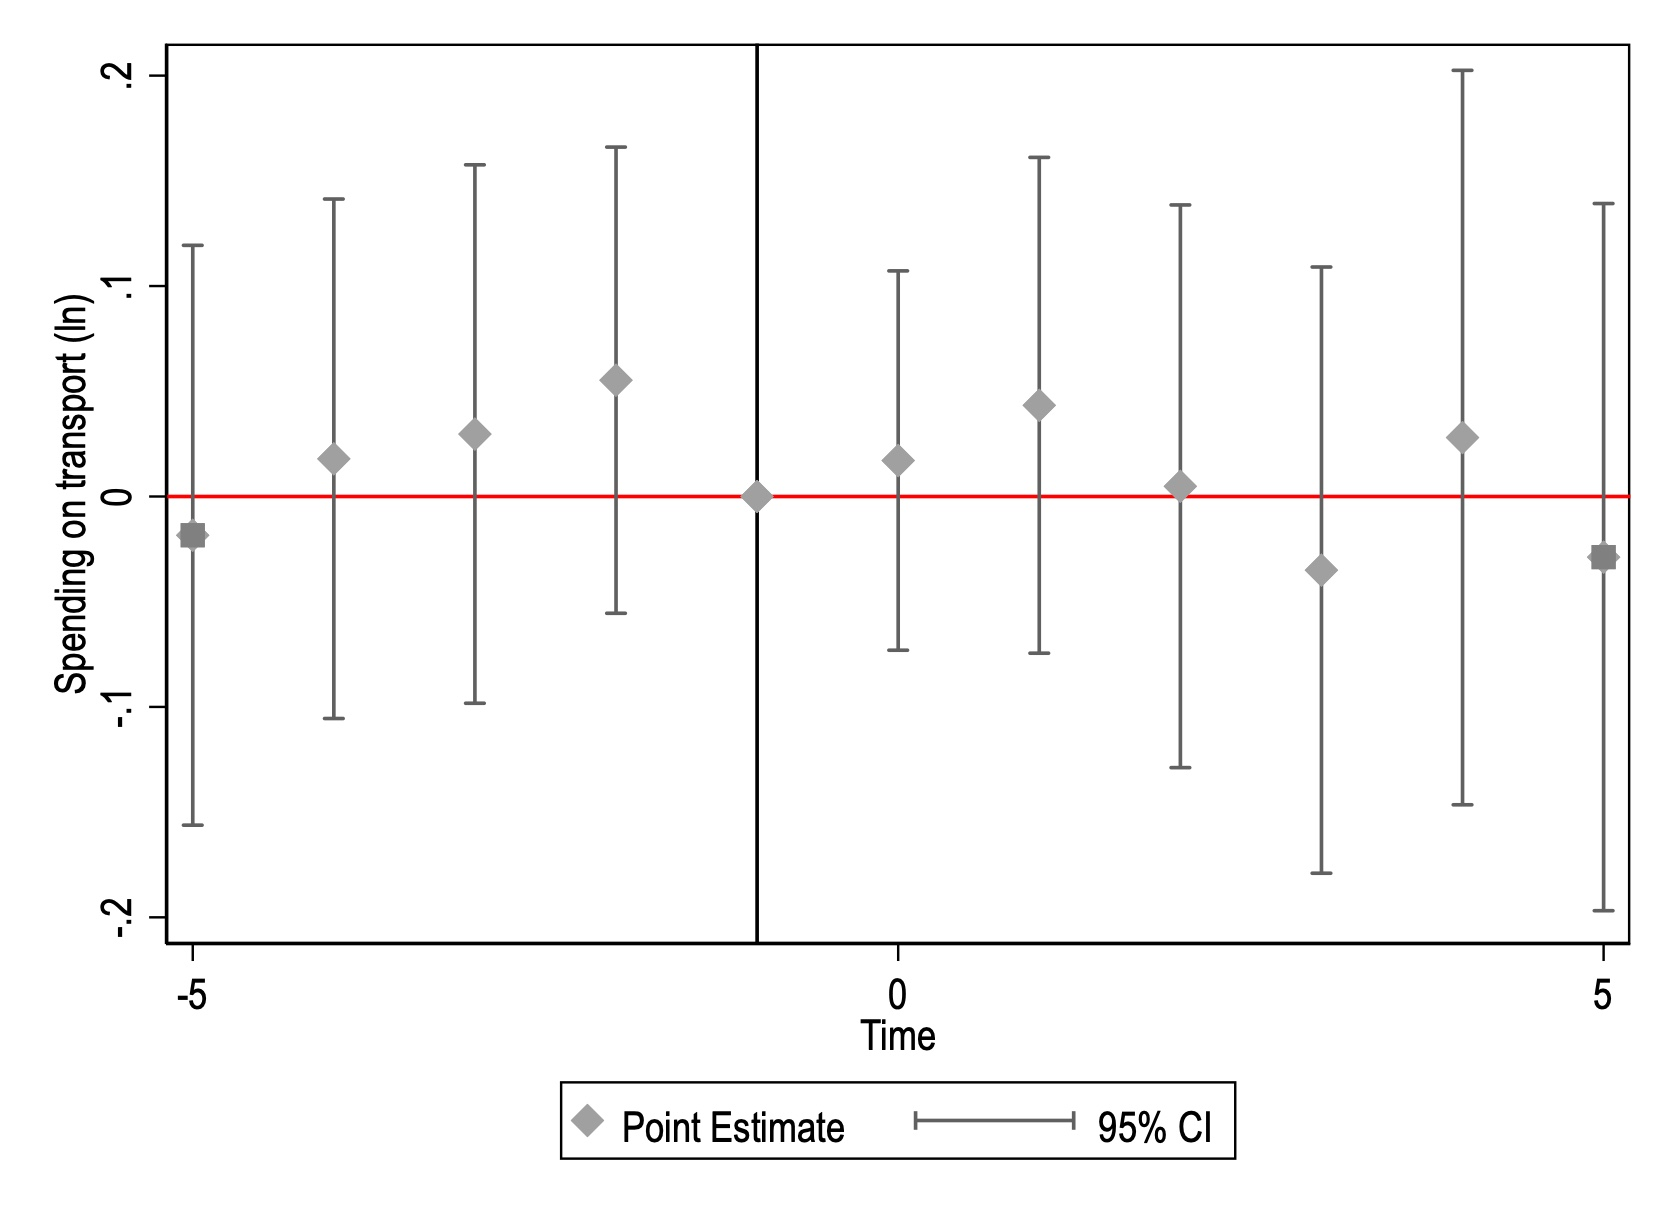
\includegraphics[width=\linewidth]{images/pop_5000/eventdd_ln_q4_08_step1.jpg}
            \label{fig:transport}
        \end{minipage} \\[10pt]

        \begin{minipage}[t]{0.32\textwidth}
            \centering
            \caption{Justice}
            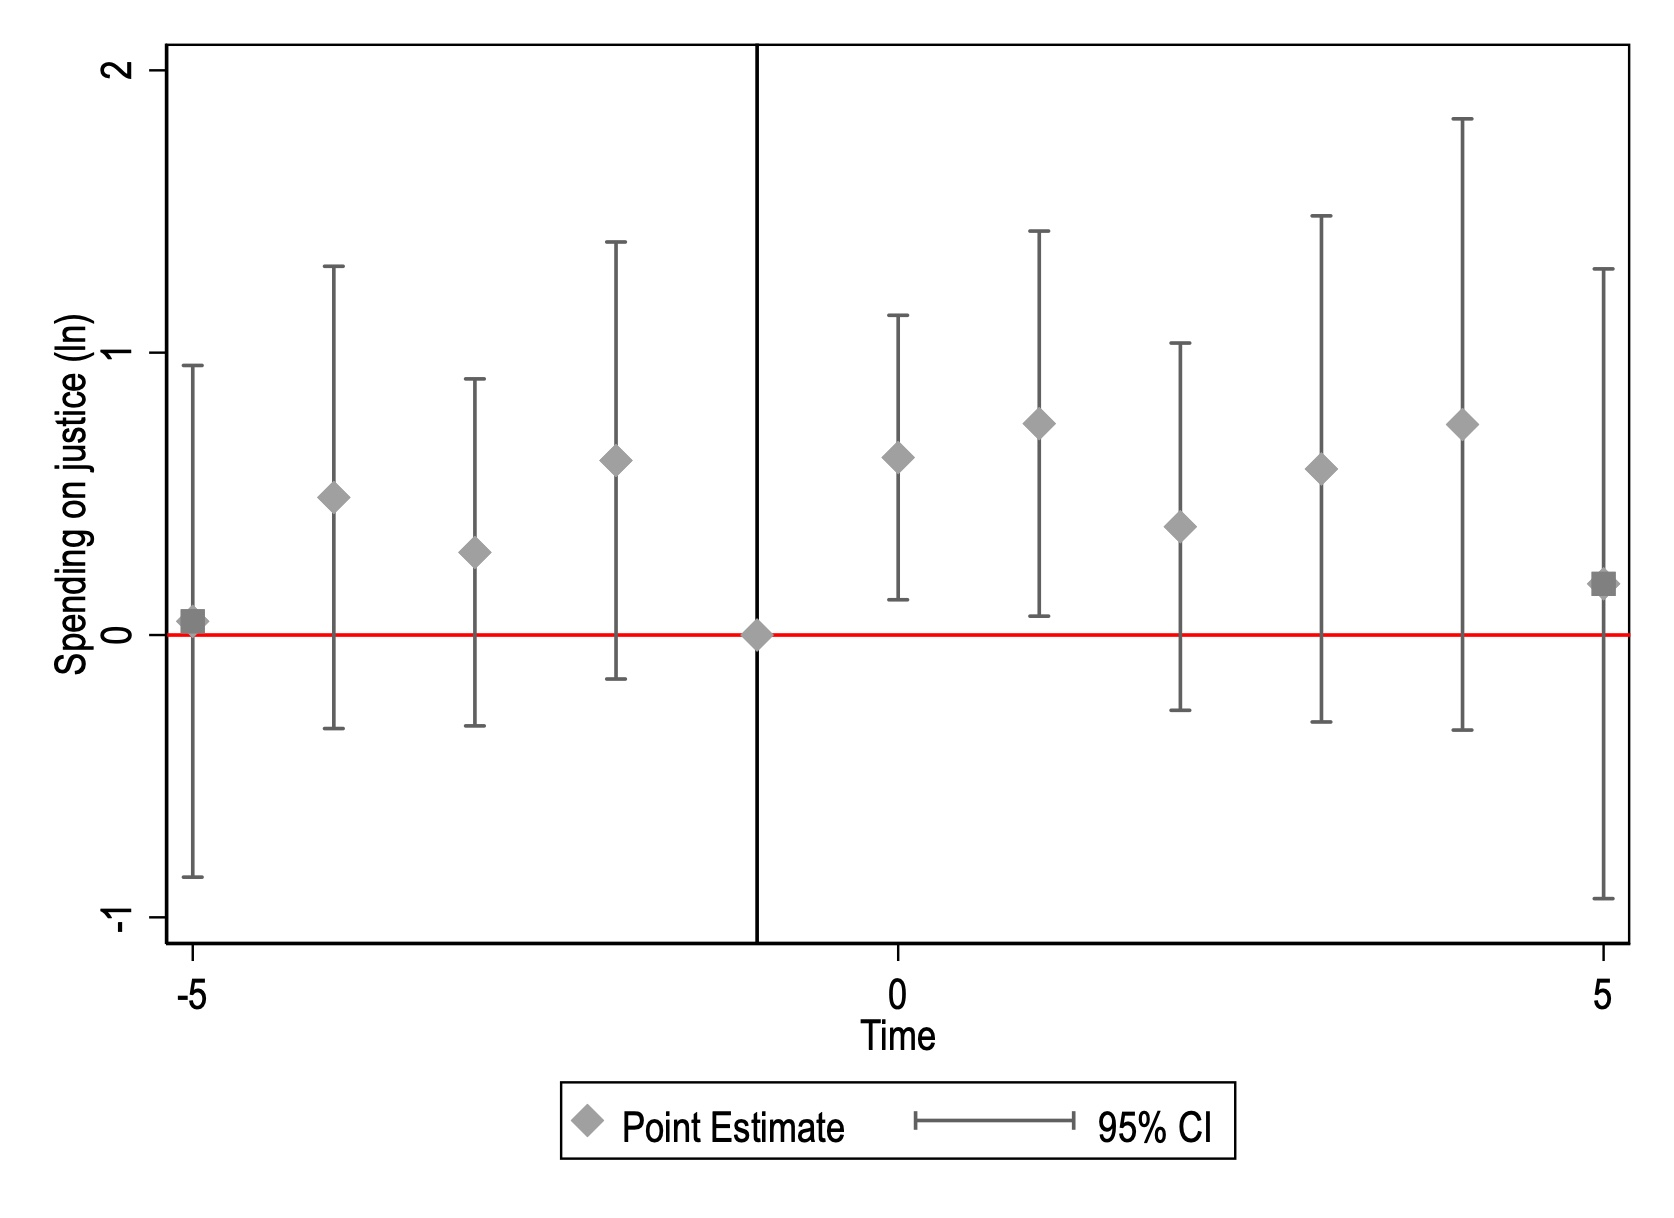
\includegraphics[width=\linewidth]{images/pop_5000/eventdd_ln_q4_02_step1.jpg}
            \label{fig:justice}
        \end{minipage} &
        \begin{minipage}[t]{0.32\textwidth}
            \centering
            \caption{Police}
            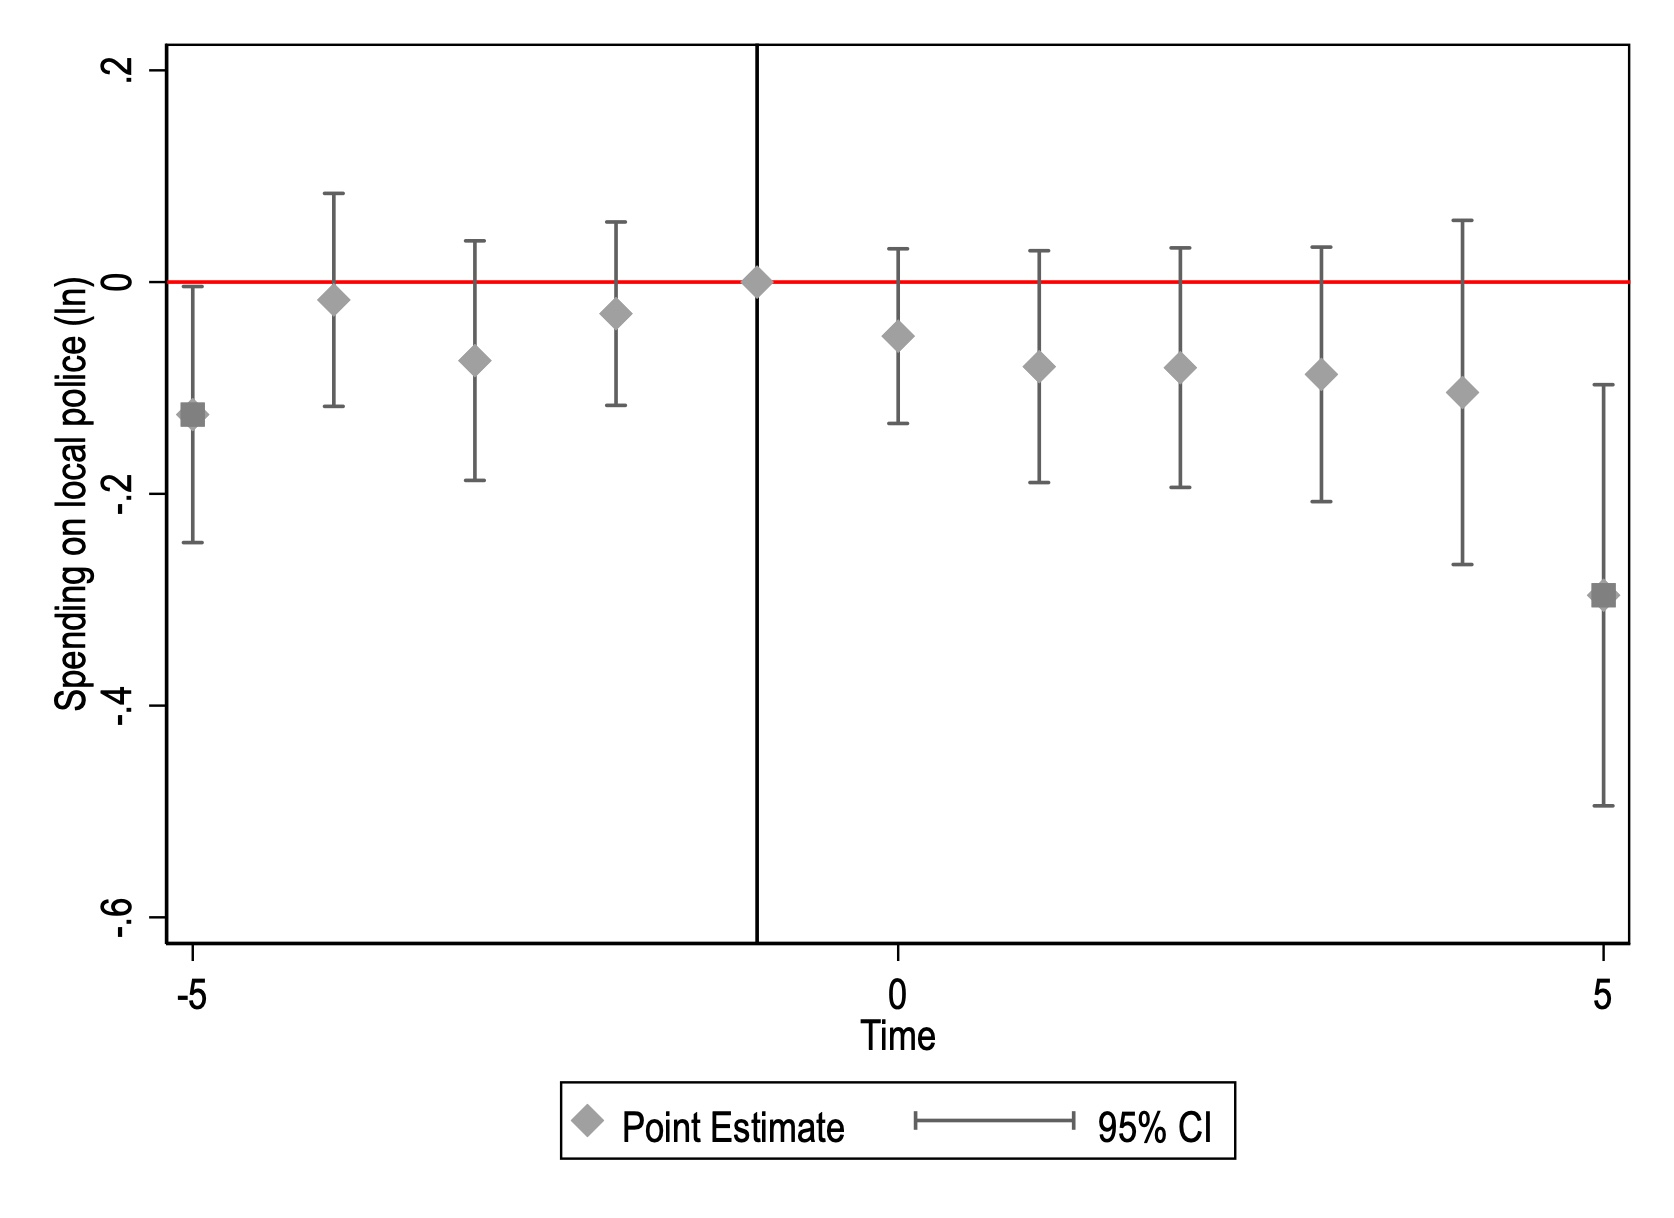
\includegraphics[width=\linewidth]{images/pop_5000/eventdd_ln_q4_03_step1.jpg}
            \label{fig:police}
        \end{minipage} &
        \begin{minipage}[t]{0.32\textwidth}
            \centering
            \caption{Culture, libraries, museums}
            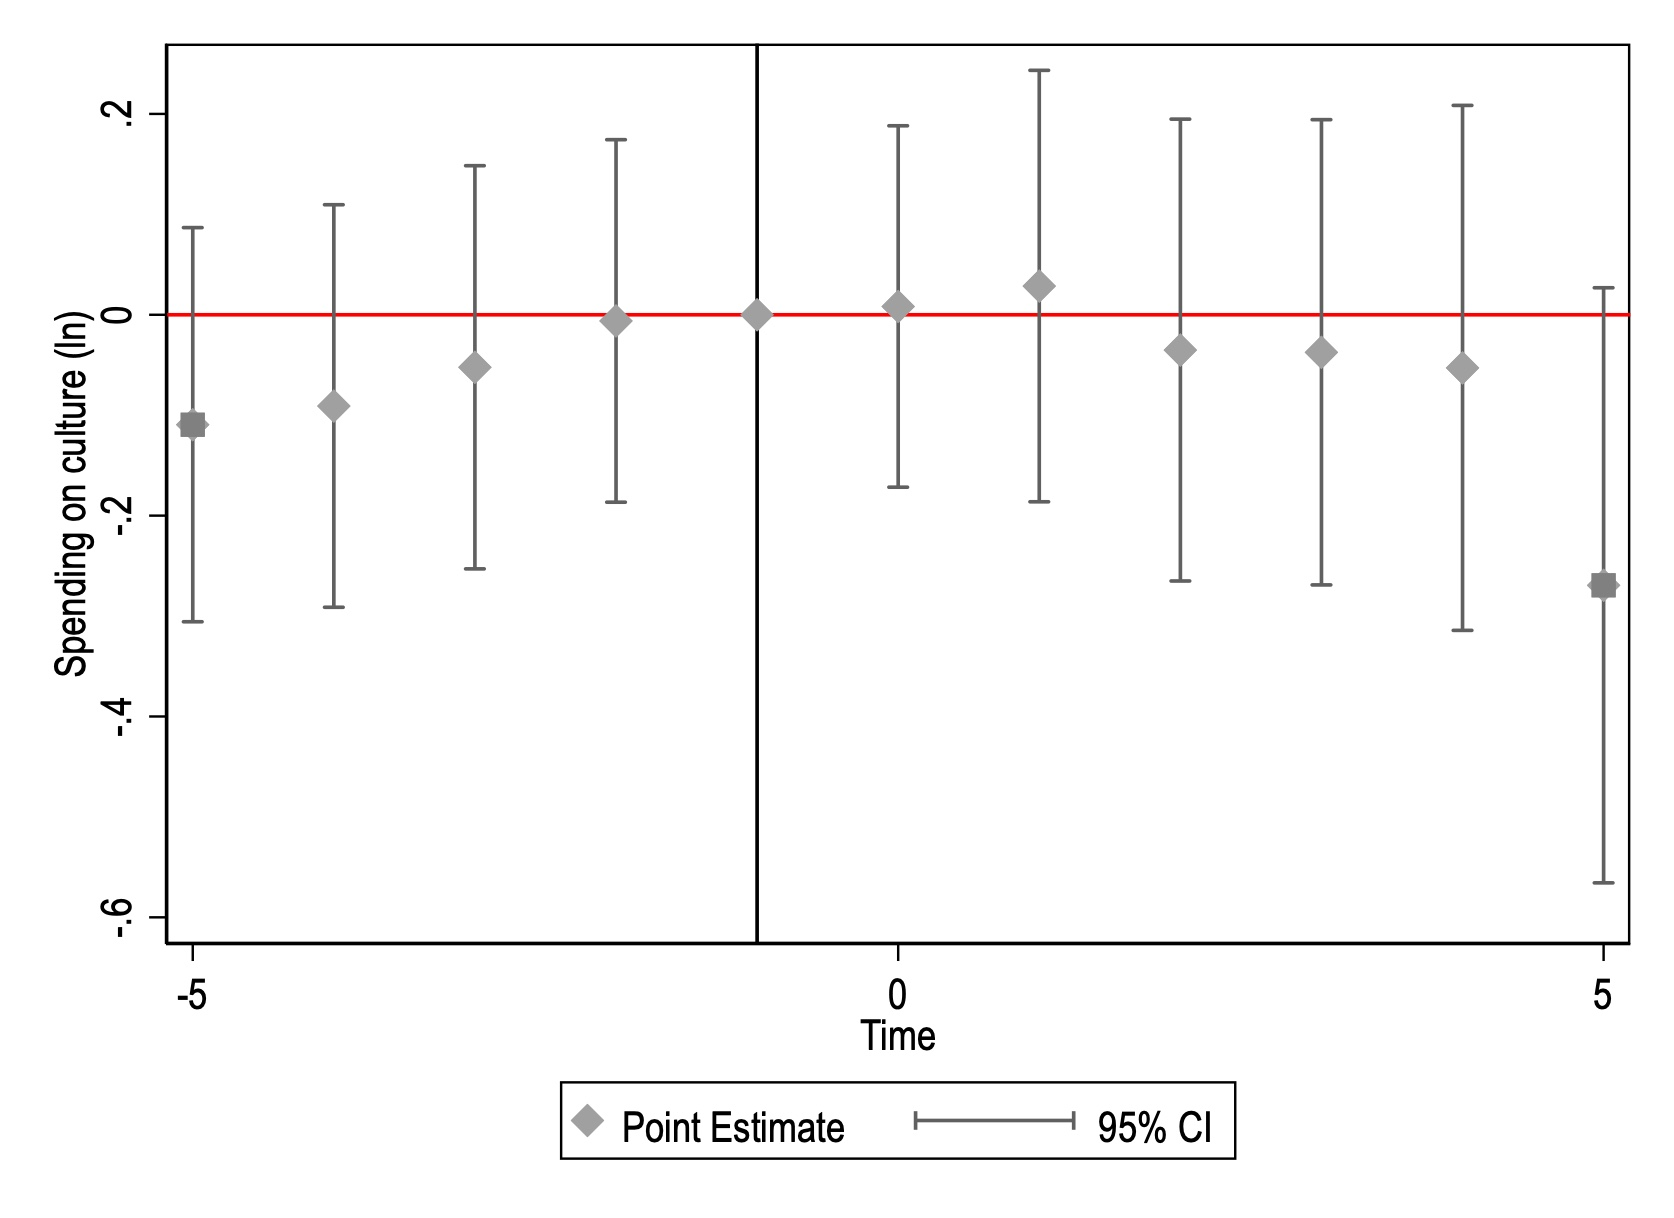
\includegraphics[width=\linewidth]{images/pop_5000/eventdd_ln_q4_05_step1.jpg}
            \label{fig:culture}
        \end{minipage} \\[10pt]

        \begin{minipage}[t]{0.32\textwidth}
            \centering
            \caption{Social services}
            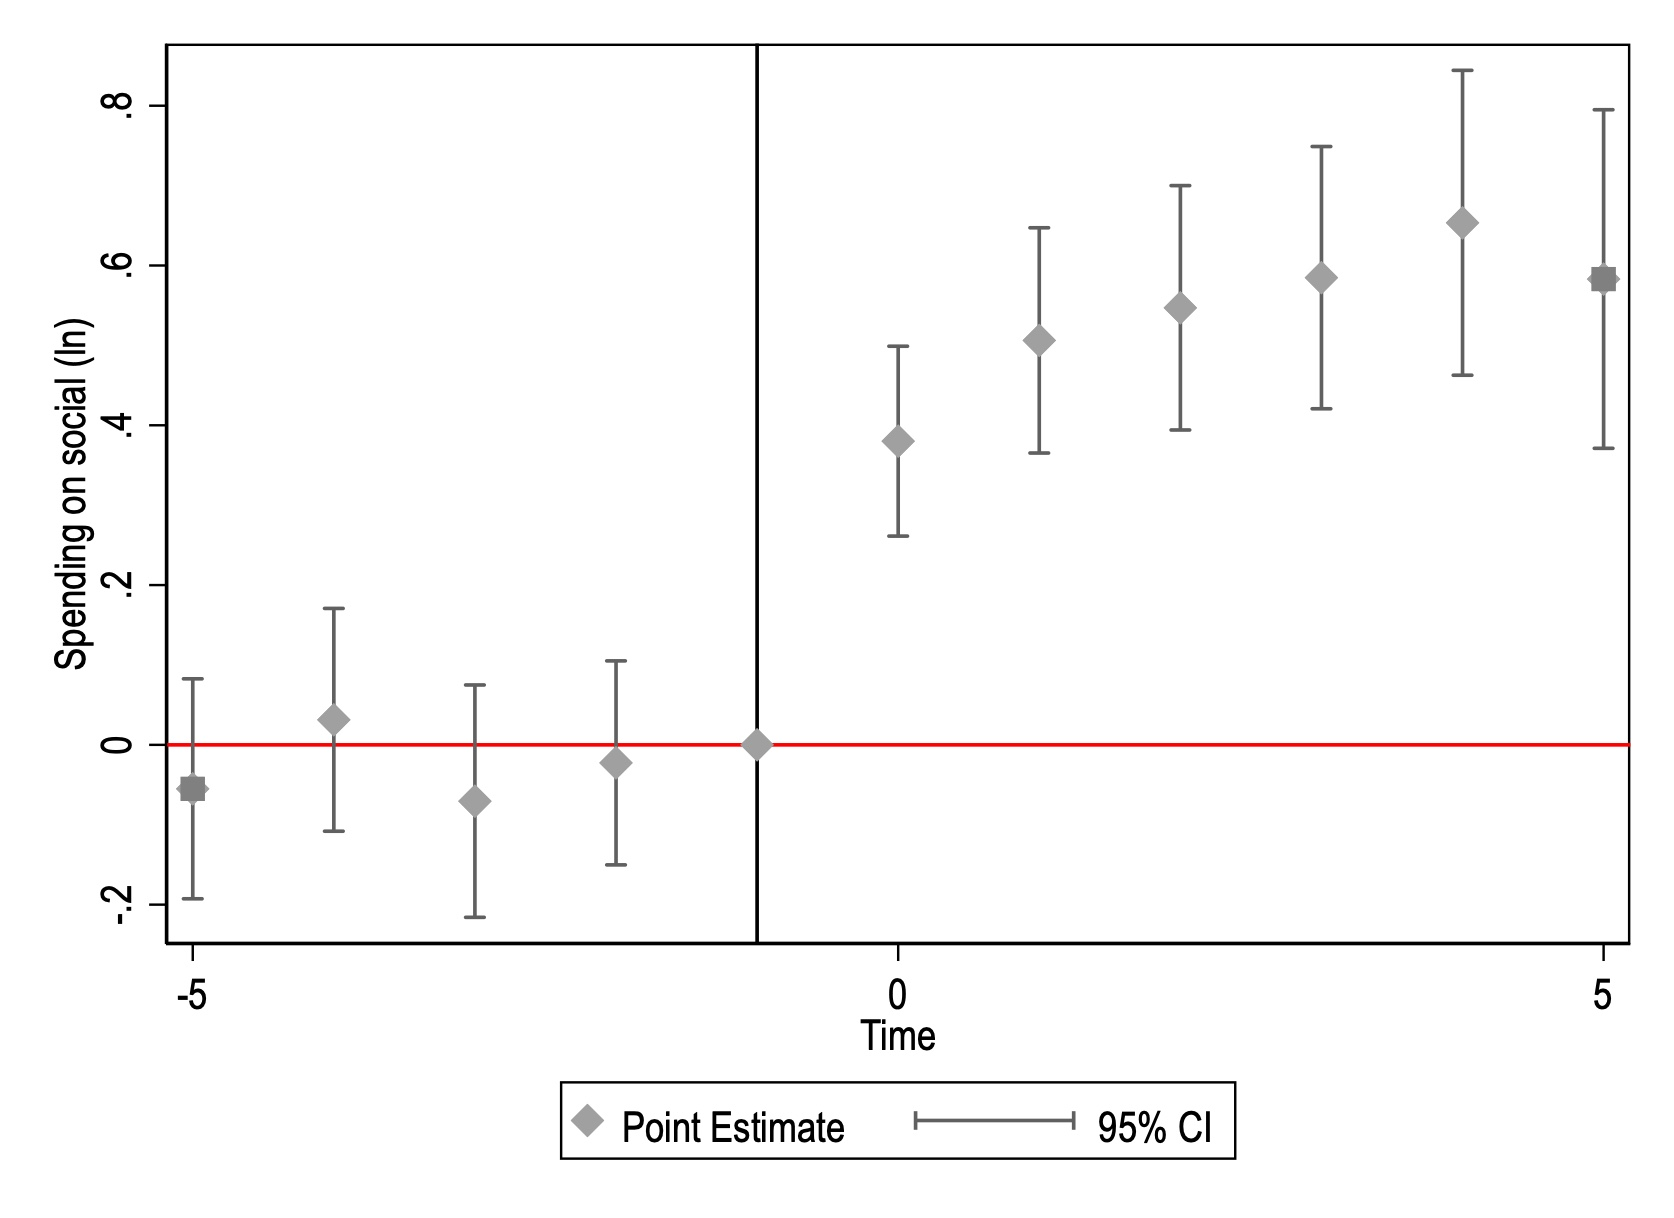
\includegraphics[width=\linewidth]{images/pop_5000/eventdd_ln_q4_10_step1.jpg}
            \label{fig:social_services}
        \end{minipage} &
        \begin{minipage}[t]{0.32\textwidth}
            \centering
            \caption{Education}
            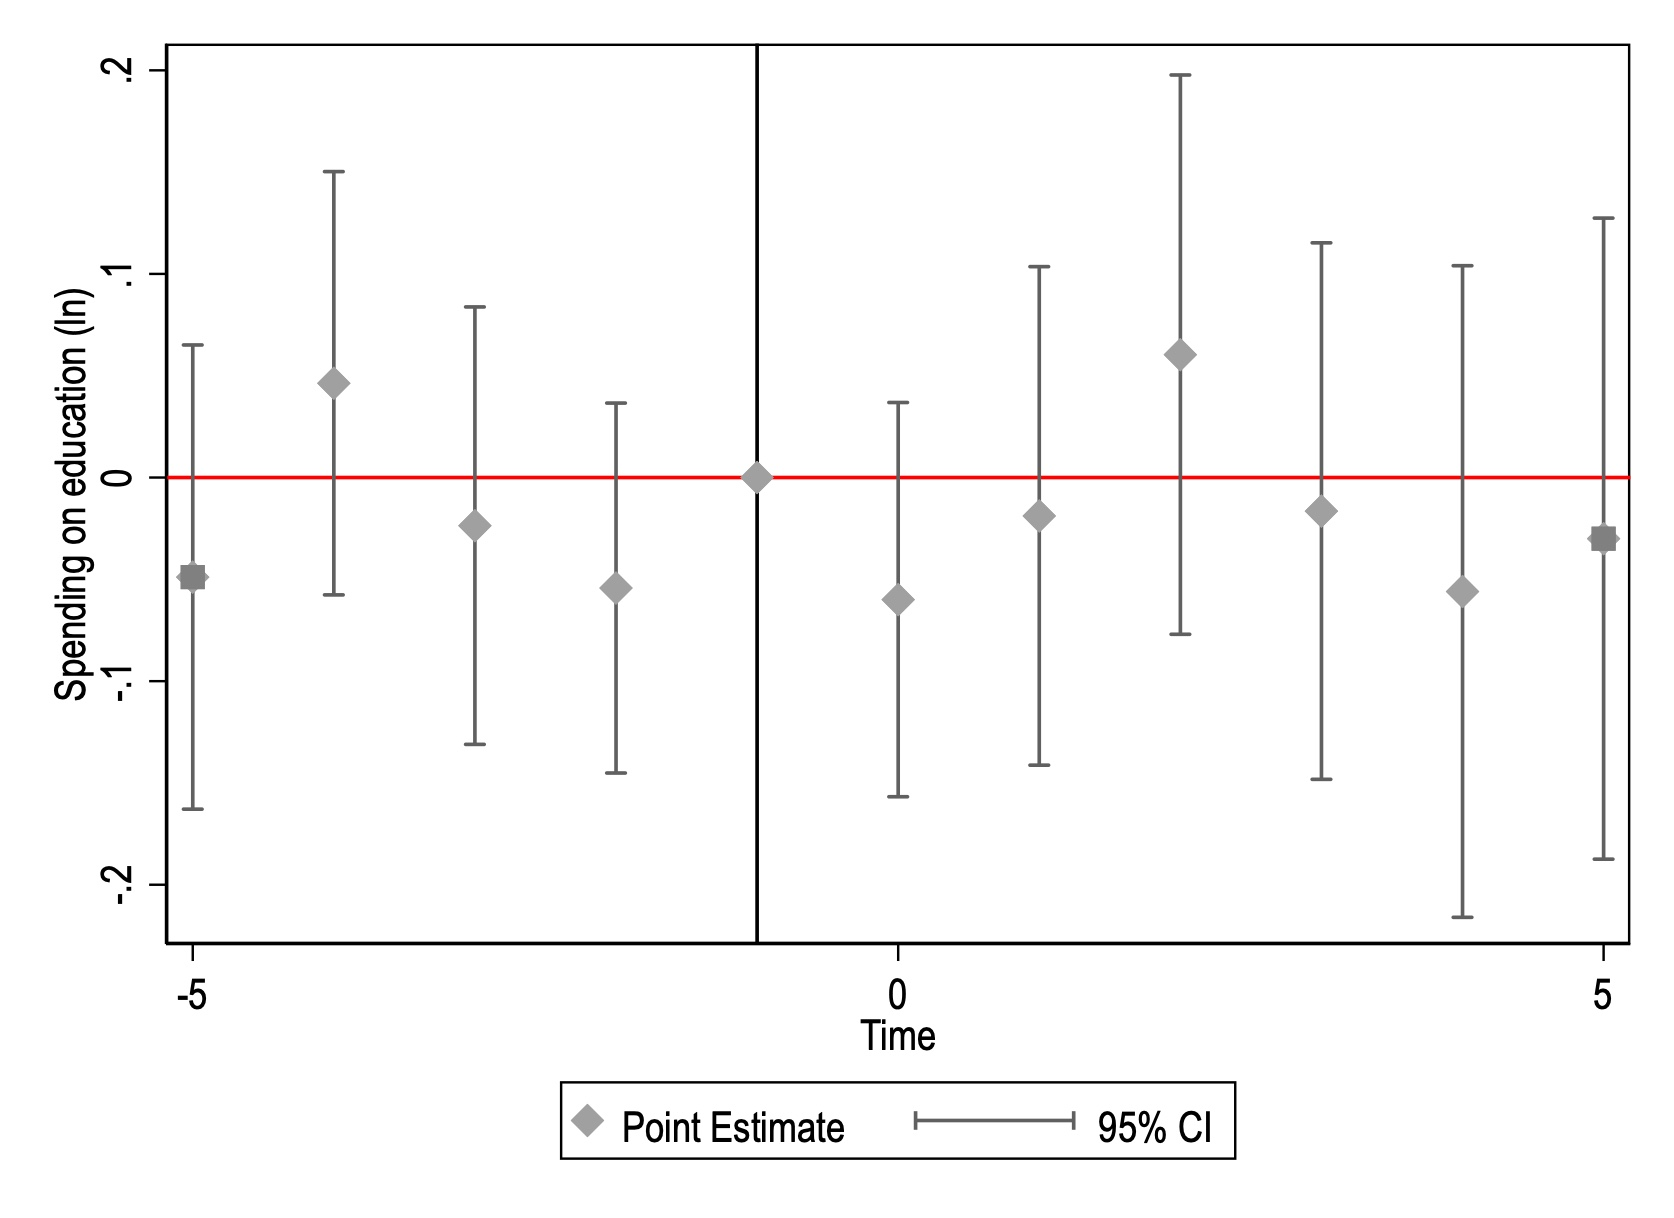
\includegraphics[width=\linewidth]{images/pop_5000/eventdd_ln_q4_04_step1.jpg}
            \label{fig:education}
        \end{minipage} &
        \begin{minipage}[t]{0.32\textwidth}
            \centering
            \caption{Economic development}
            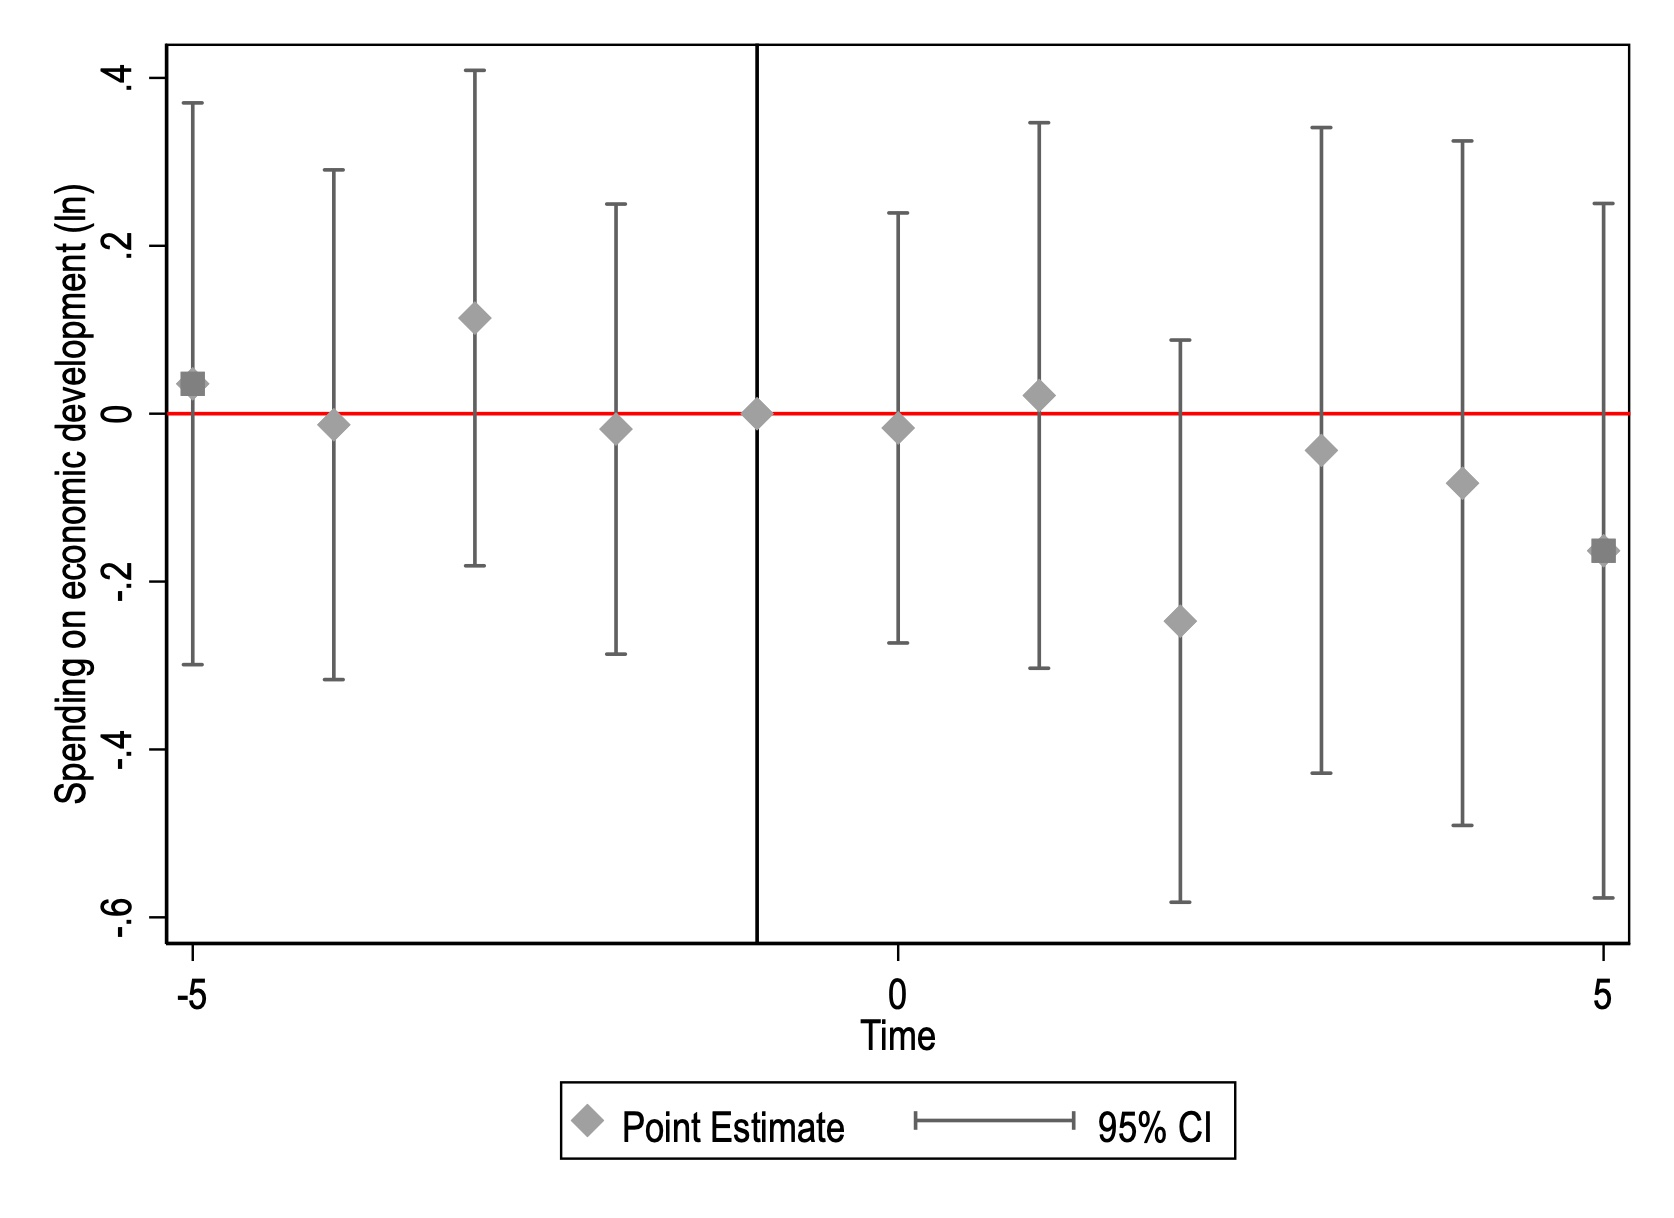
\includegraphics[width=\linewidth]{images/pop_5000/eventdd_ln_q4_11_step1.jpg}
            \label{fig:ecodev}
        \end{minipage} \\[10pt]

        \begin{minipage}[t]{0.32\textwidth}
            \centering
            \caption{Production services}
            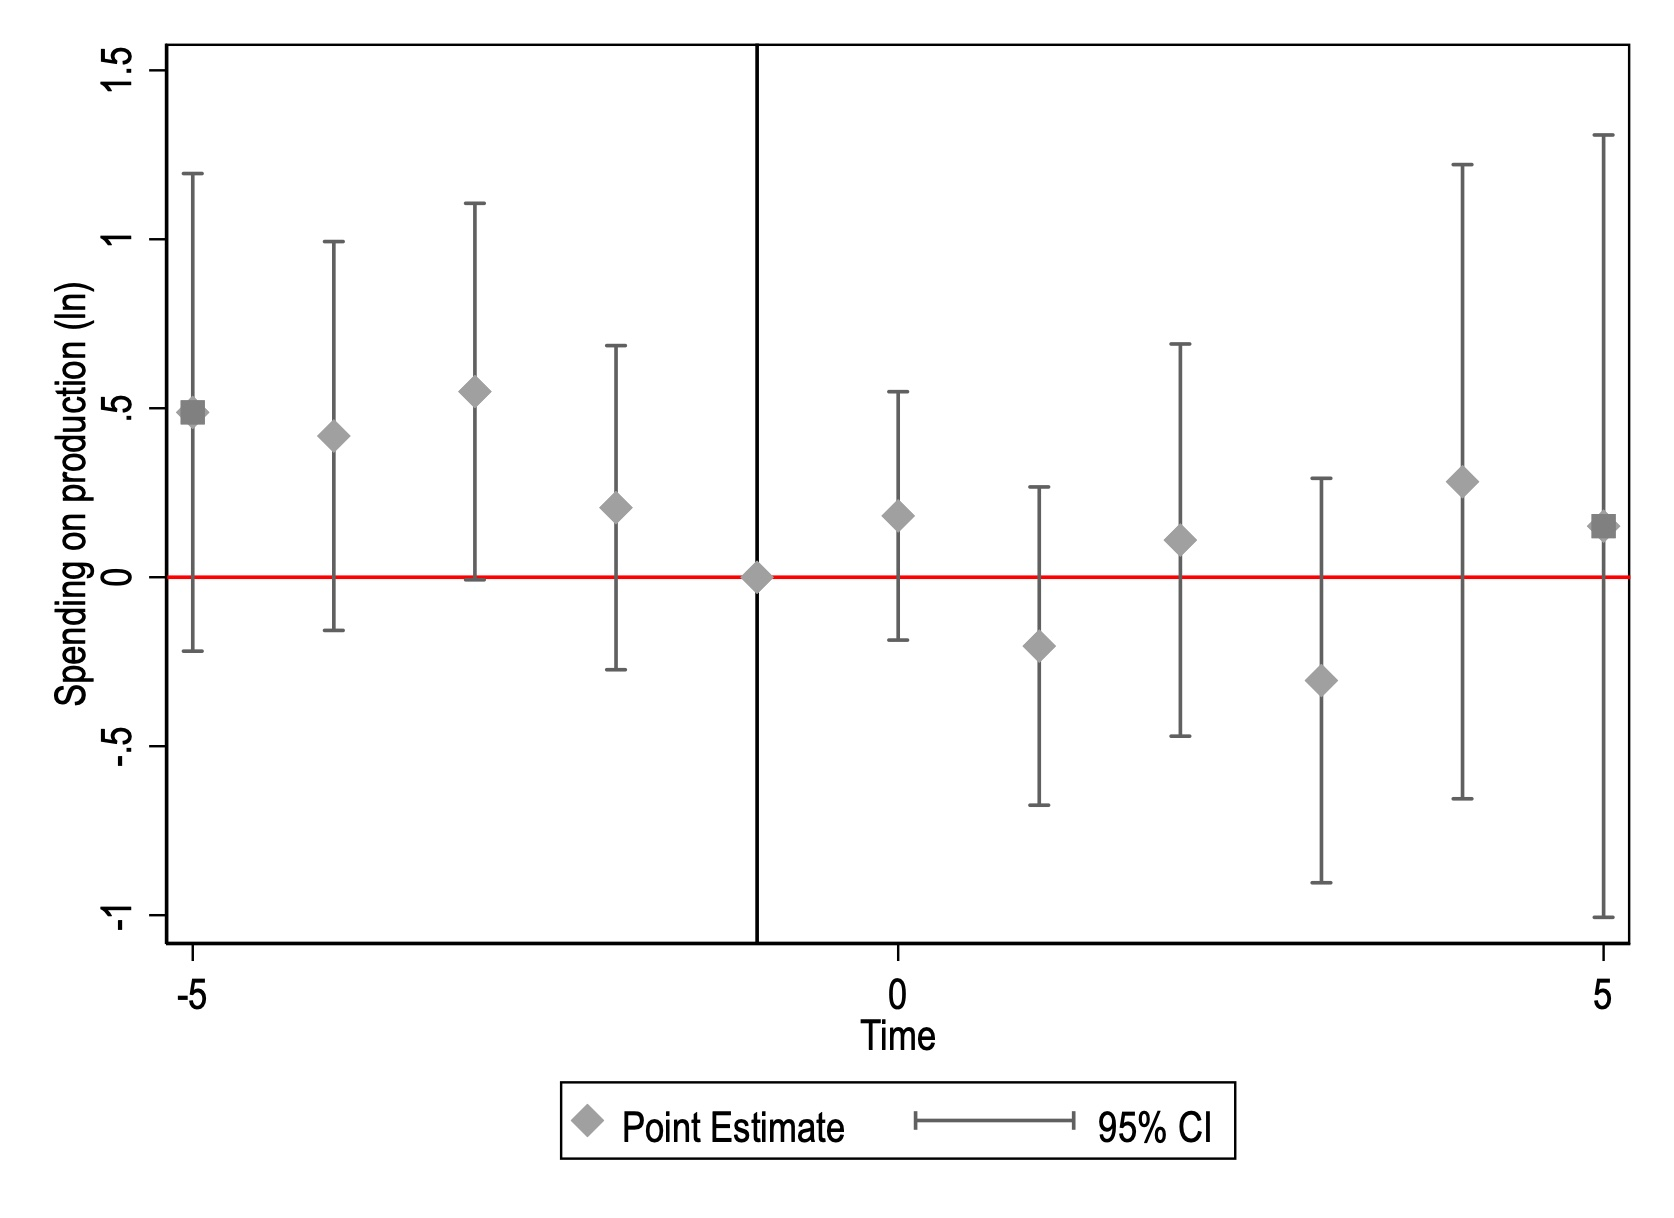
\includegraphics[width=\linewidth]{images/pop_5000/eventdd_ln_q4_12_step1.jpg}
            \label{fig:production}
        \end{minipage} &
        \begin{minipage}[t]{0.32\textwidth}
            \centering
            \caption{Administrative services}
            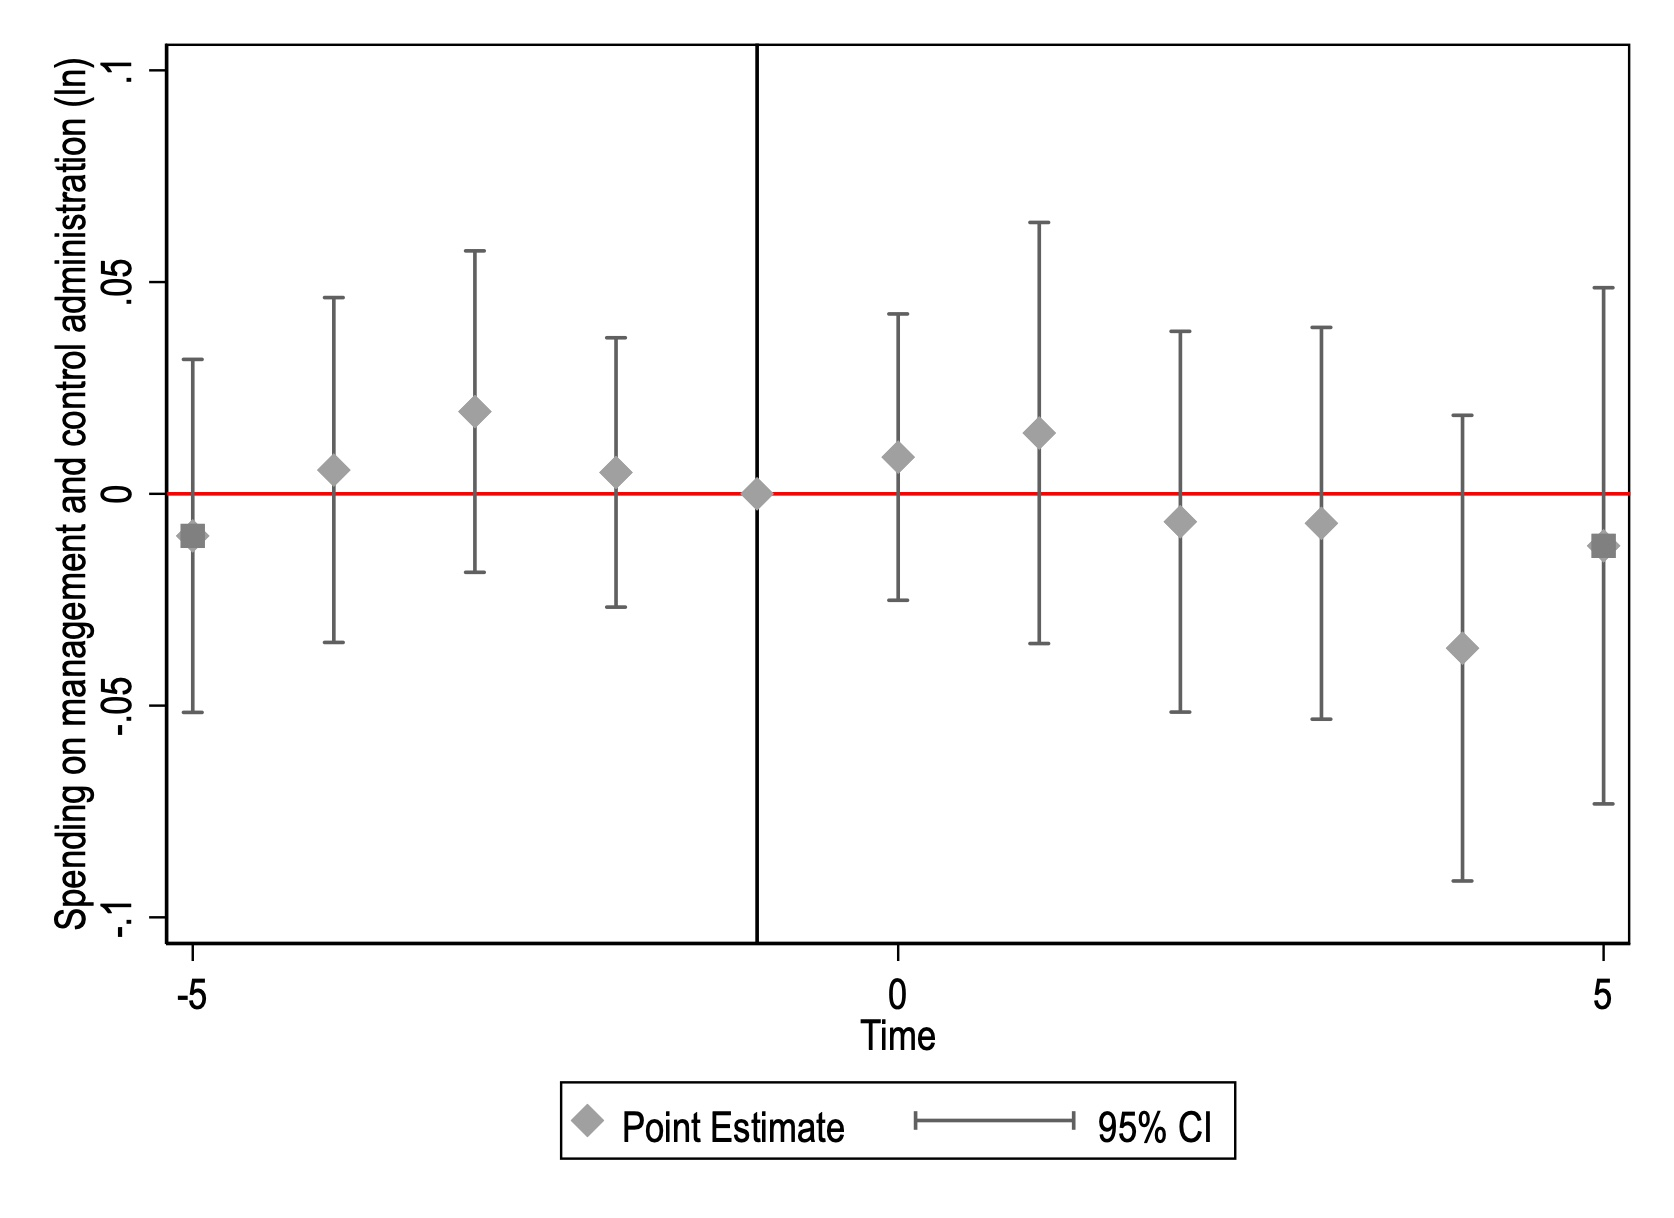
\includegraphics[width=\linewidth]{images/pop_5000/eventdd_ln_q4_01_step1.jpg}
            \label{fig:administration}
        \end{minipage} &
        \begin{minipage}[t]{0.32\textwidth}
            \centering
            \caption{Environment, public parks, recycling}
            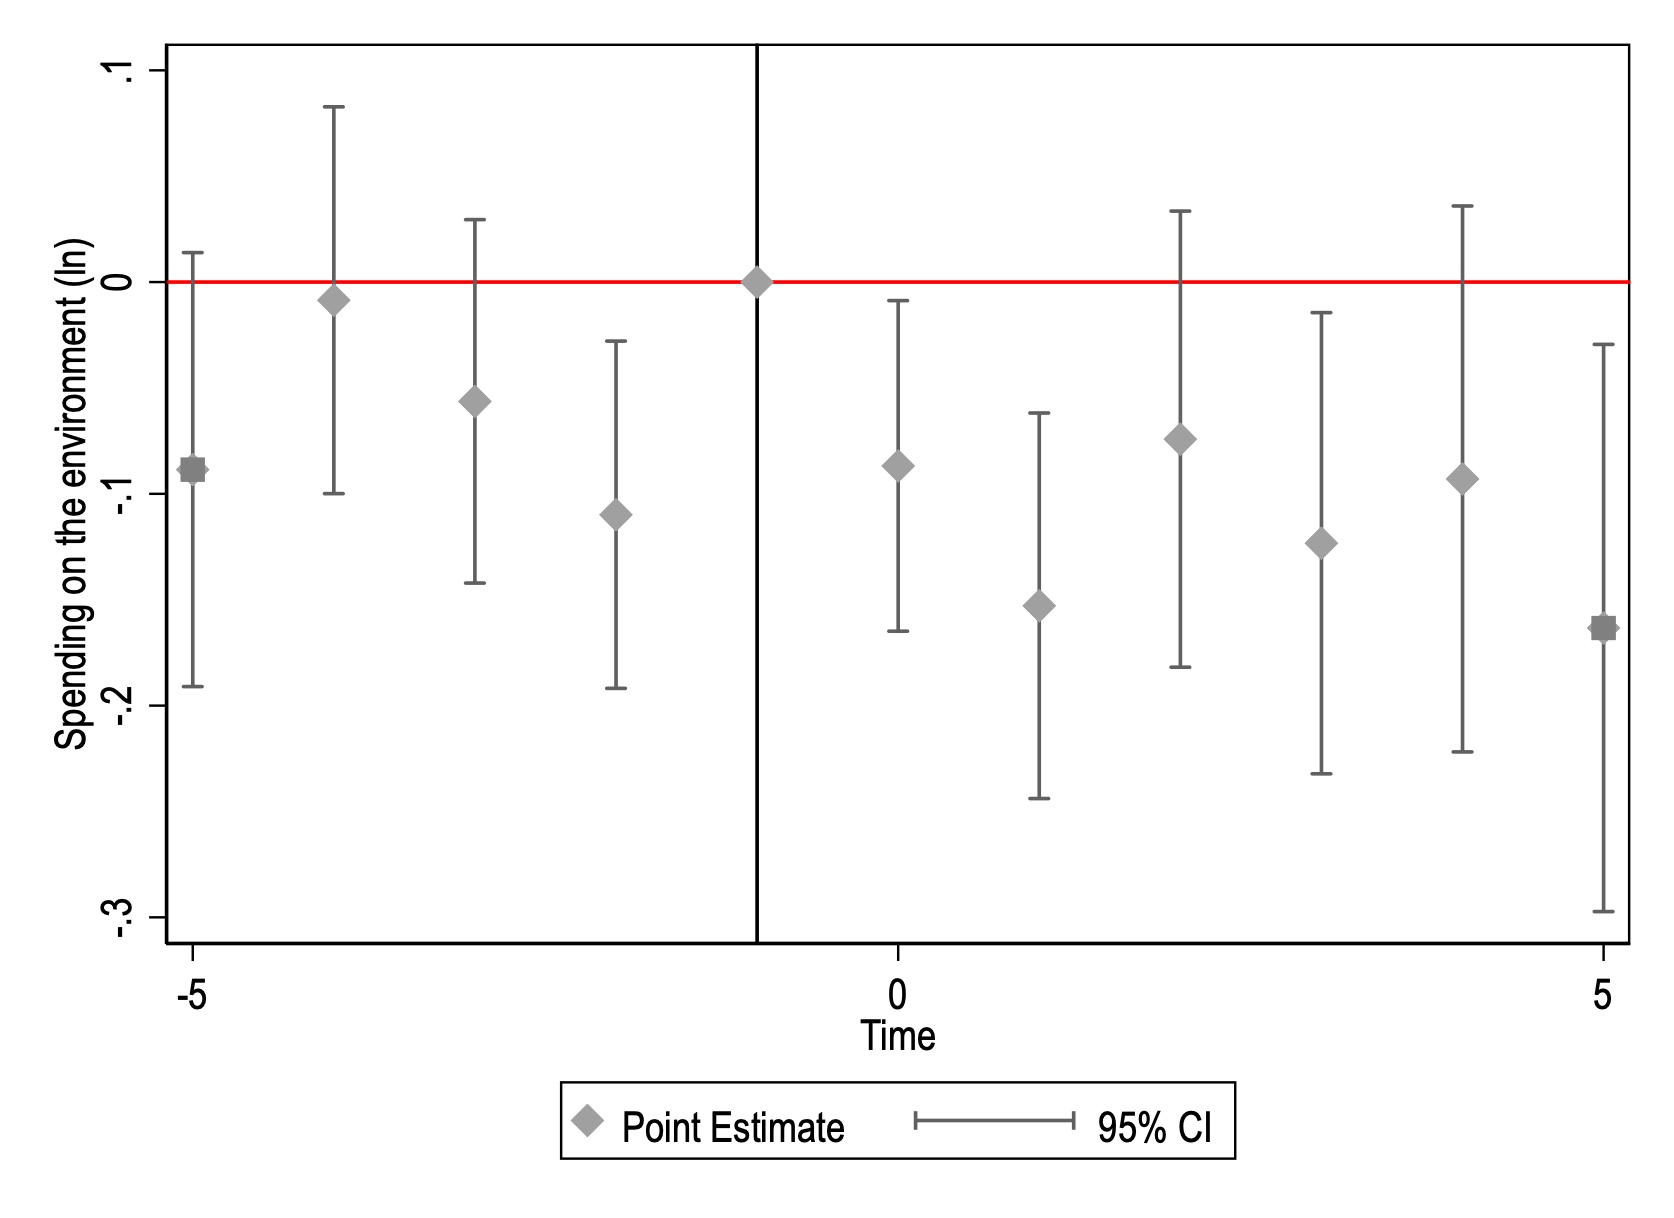
\includegraphics[width=\linewidth]{images/pop_5000/eventdd_ln_q4_09_step1.jpg}
            \label{fig:environment}
        \end{minipage}
    \end{tabular}
\end{figure}


\begin{figure}[!ht]
\fontsize{7.2}{7.2}\selectfont
    \centering
\caption*{Effect of CAS centers on municipalities' public spending}
    \begin{tabular}{@{}ccc@{}}
        \begin{minipage}[t]{0.32\textwidth}
            \centering
            \caption{Total spending}
            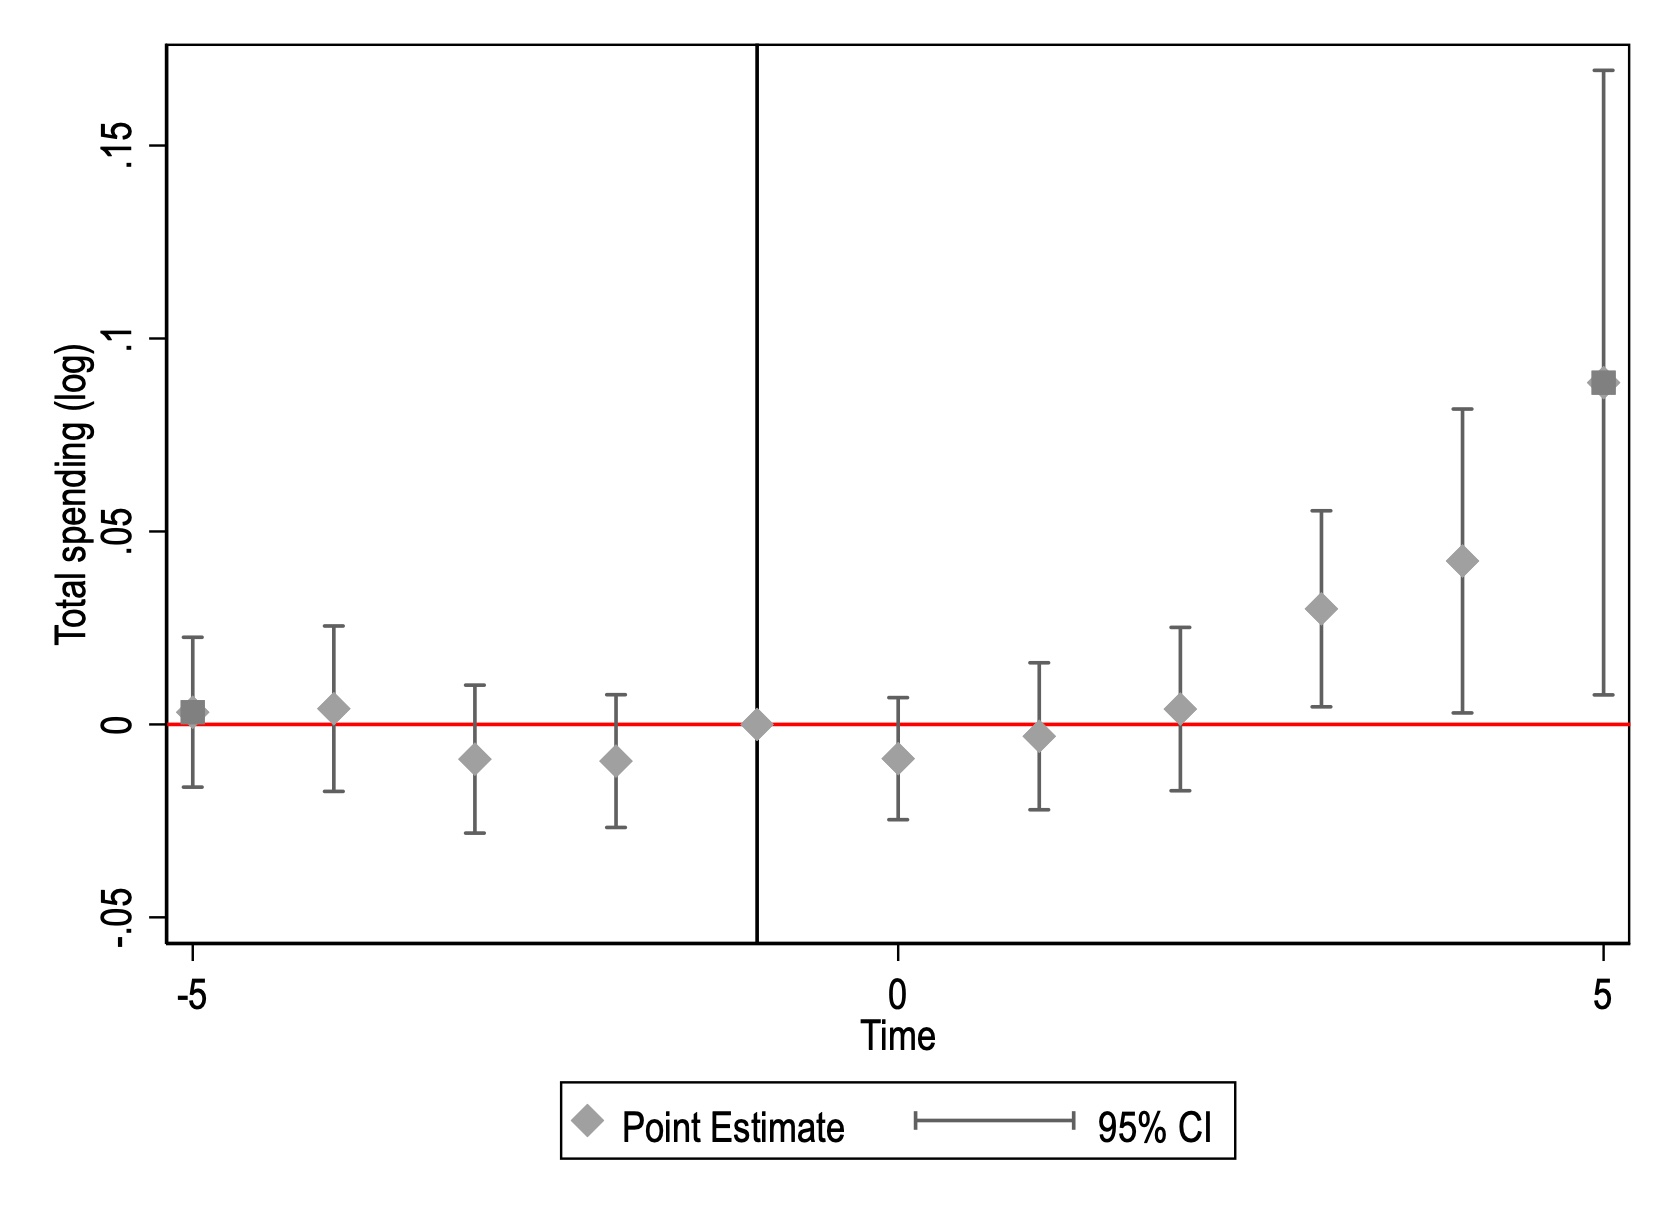
\includegraphics[width=\linewidth]{images/pop_5000/caseventdd_ln_q4tot_step1.jpg}
            \label{fig:castotal_spending}
        \end{minipage} &
        \begin{minipage}[t]{0.32\textwidth}
            \centering
            \caption{Sport}
            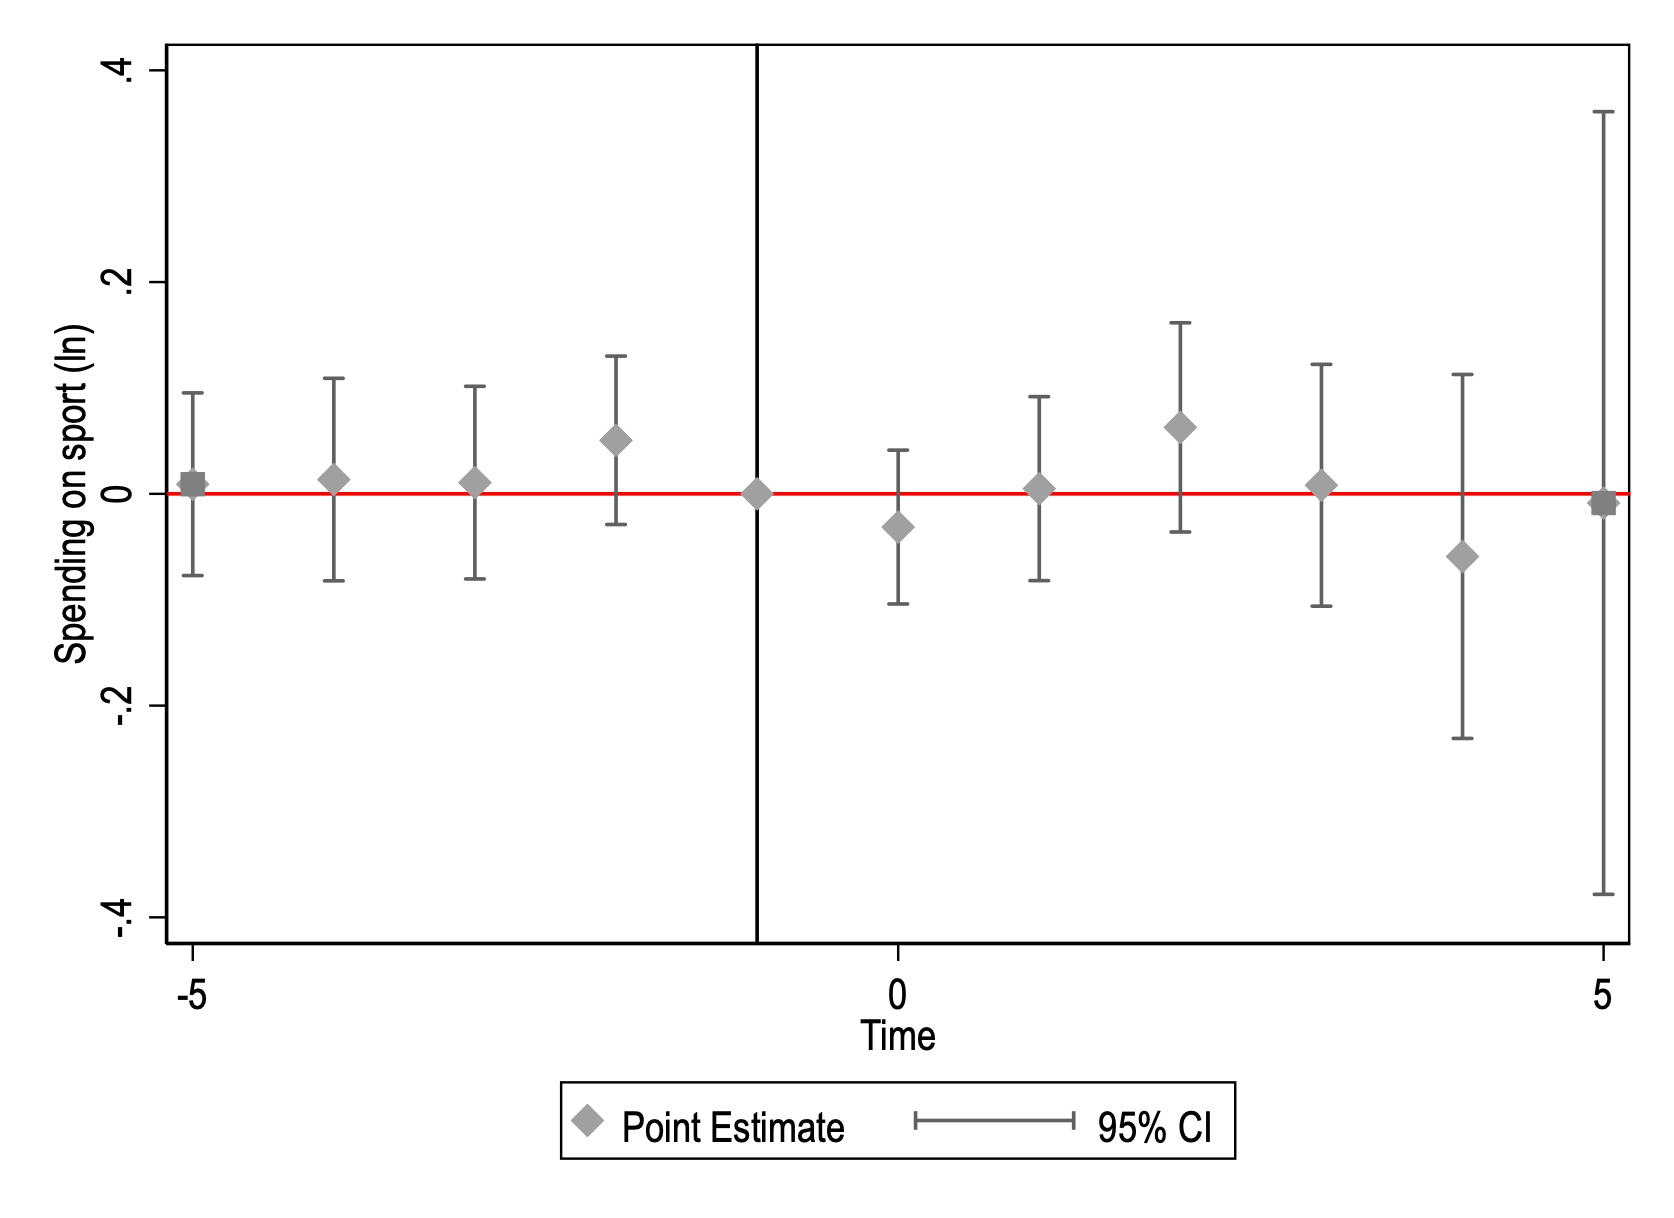
\includegraphics[width=\linewidth]{images/pop_5000/caseventdd_ln_q4_06_step1.jpg}
            \label{fig:cassport}
        \end{minipage} &
        \begin{minipage}[t]{0.32\textwidth}
            \centering
            \caption{Transport}
            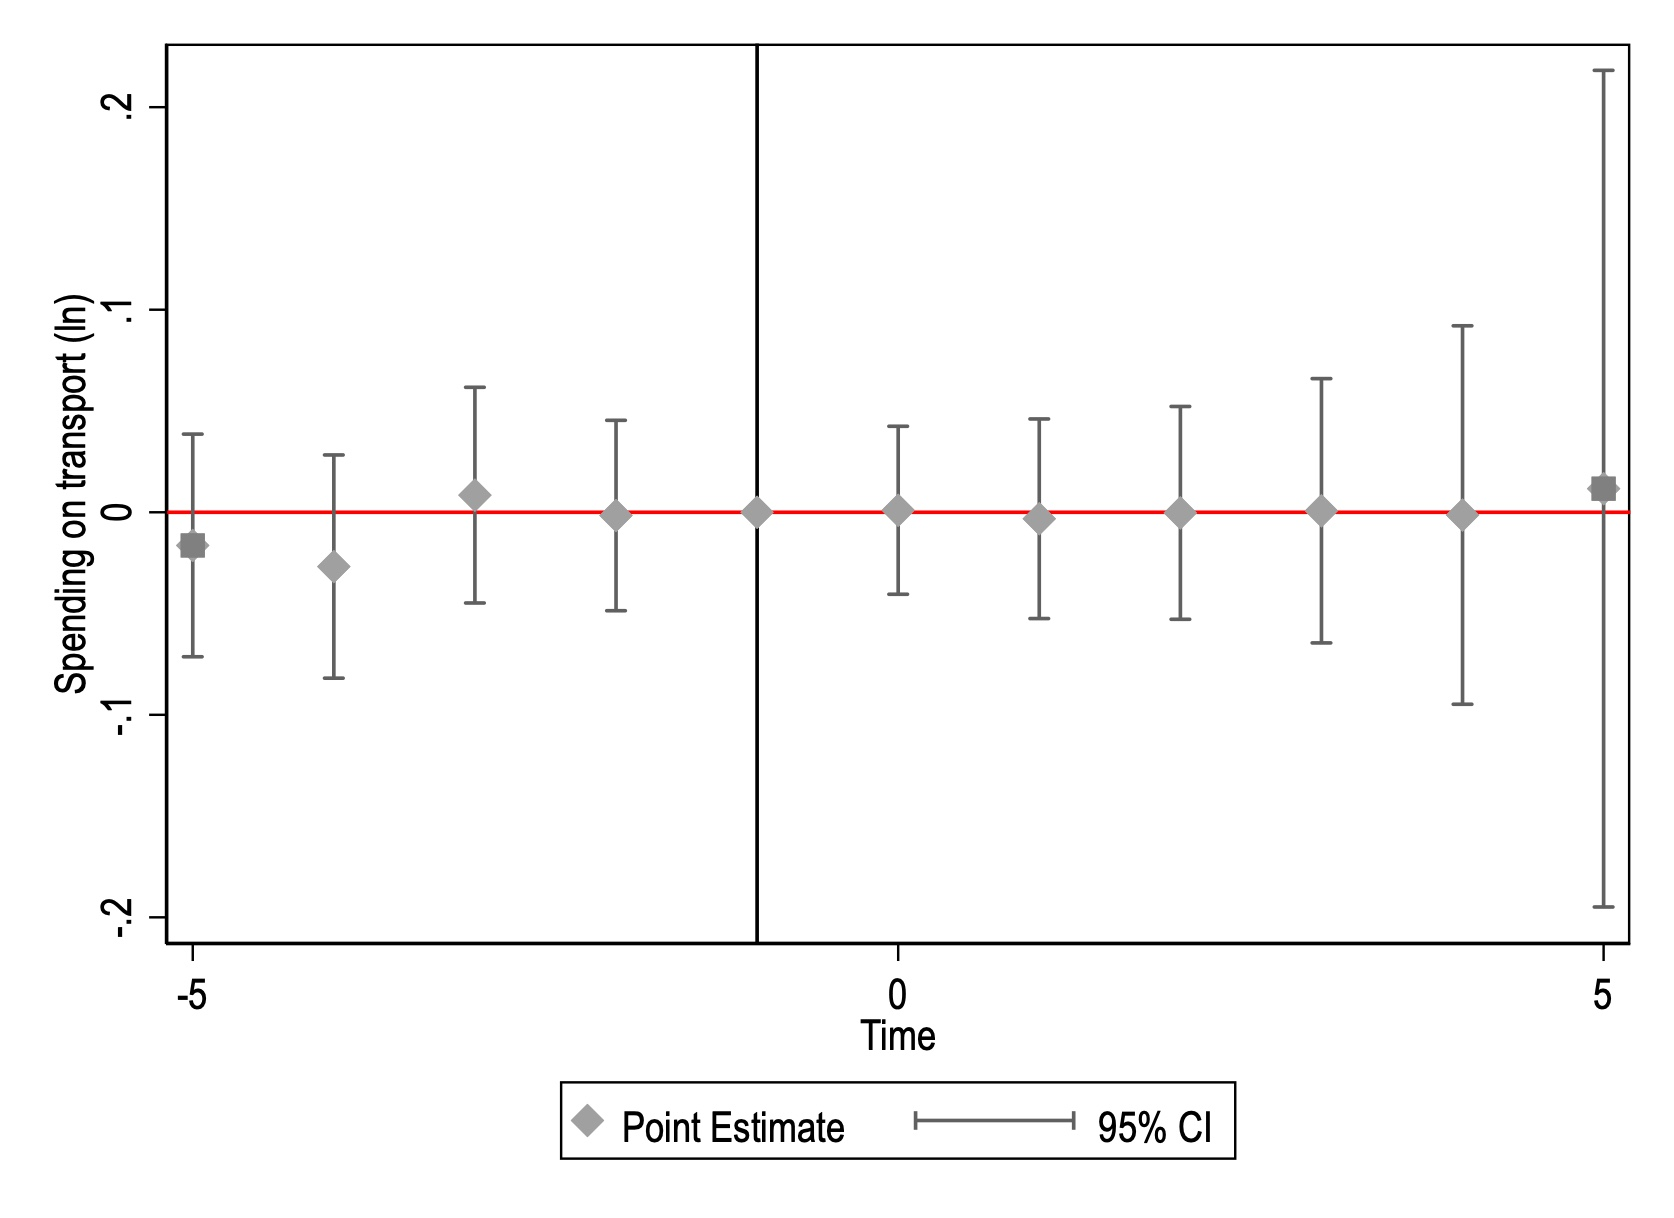
\includegraphics[width=\linewidth]{images/pop_5000/caseventdd_ln_q4_08_step1.jpg}
            \label{fig:castransport}
        \end{minipage} \\[10pt]

        \begin{minipage}[t]{0.32\textwidth}
            \centering
            \caption{Justice}
            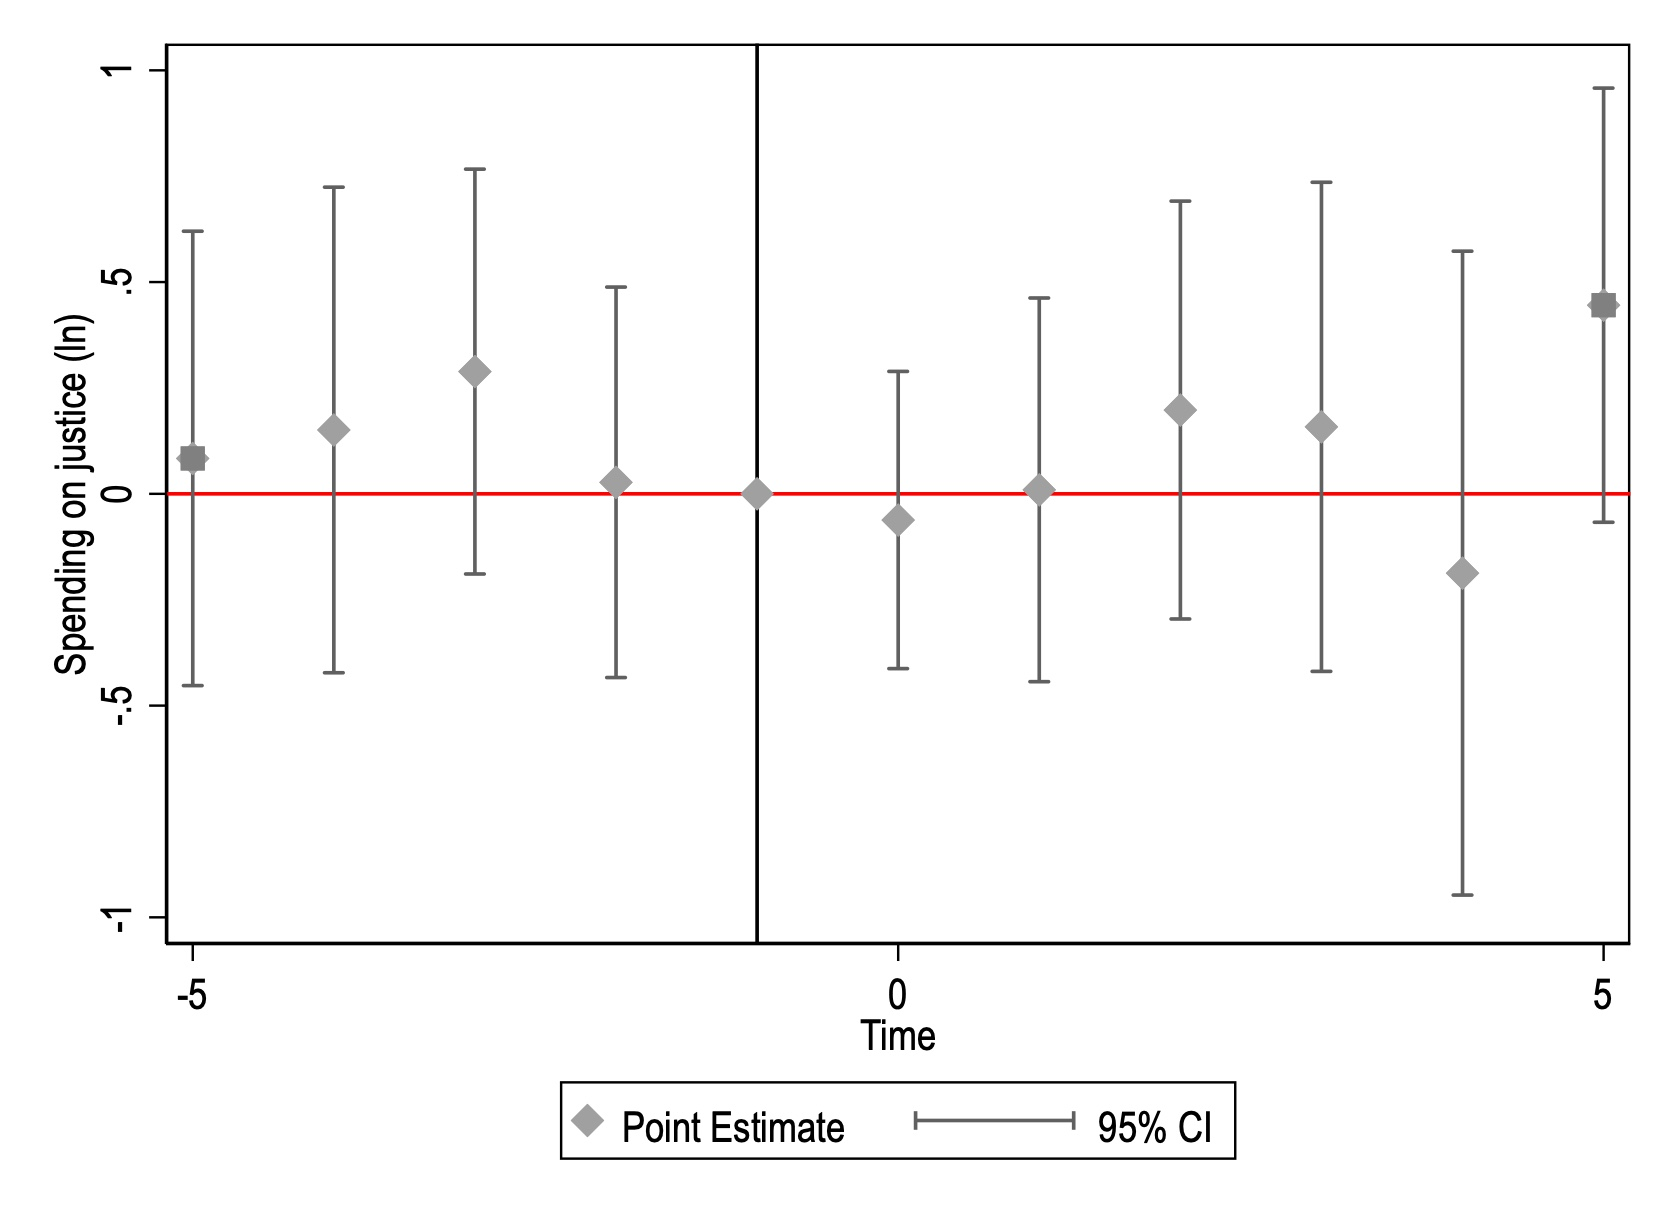
\includegraphics[width=\linewidth]{images/pop_5000/caseventdd_ln_q4_02_step1.jpg}
            \label{fig:casjustice}
        \end{minipage} &
        \begin{minipage}[t]{0.32\textwidth}
            \centering
            \caption{Police}
            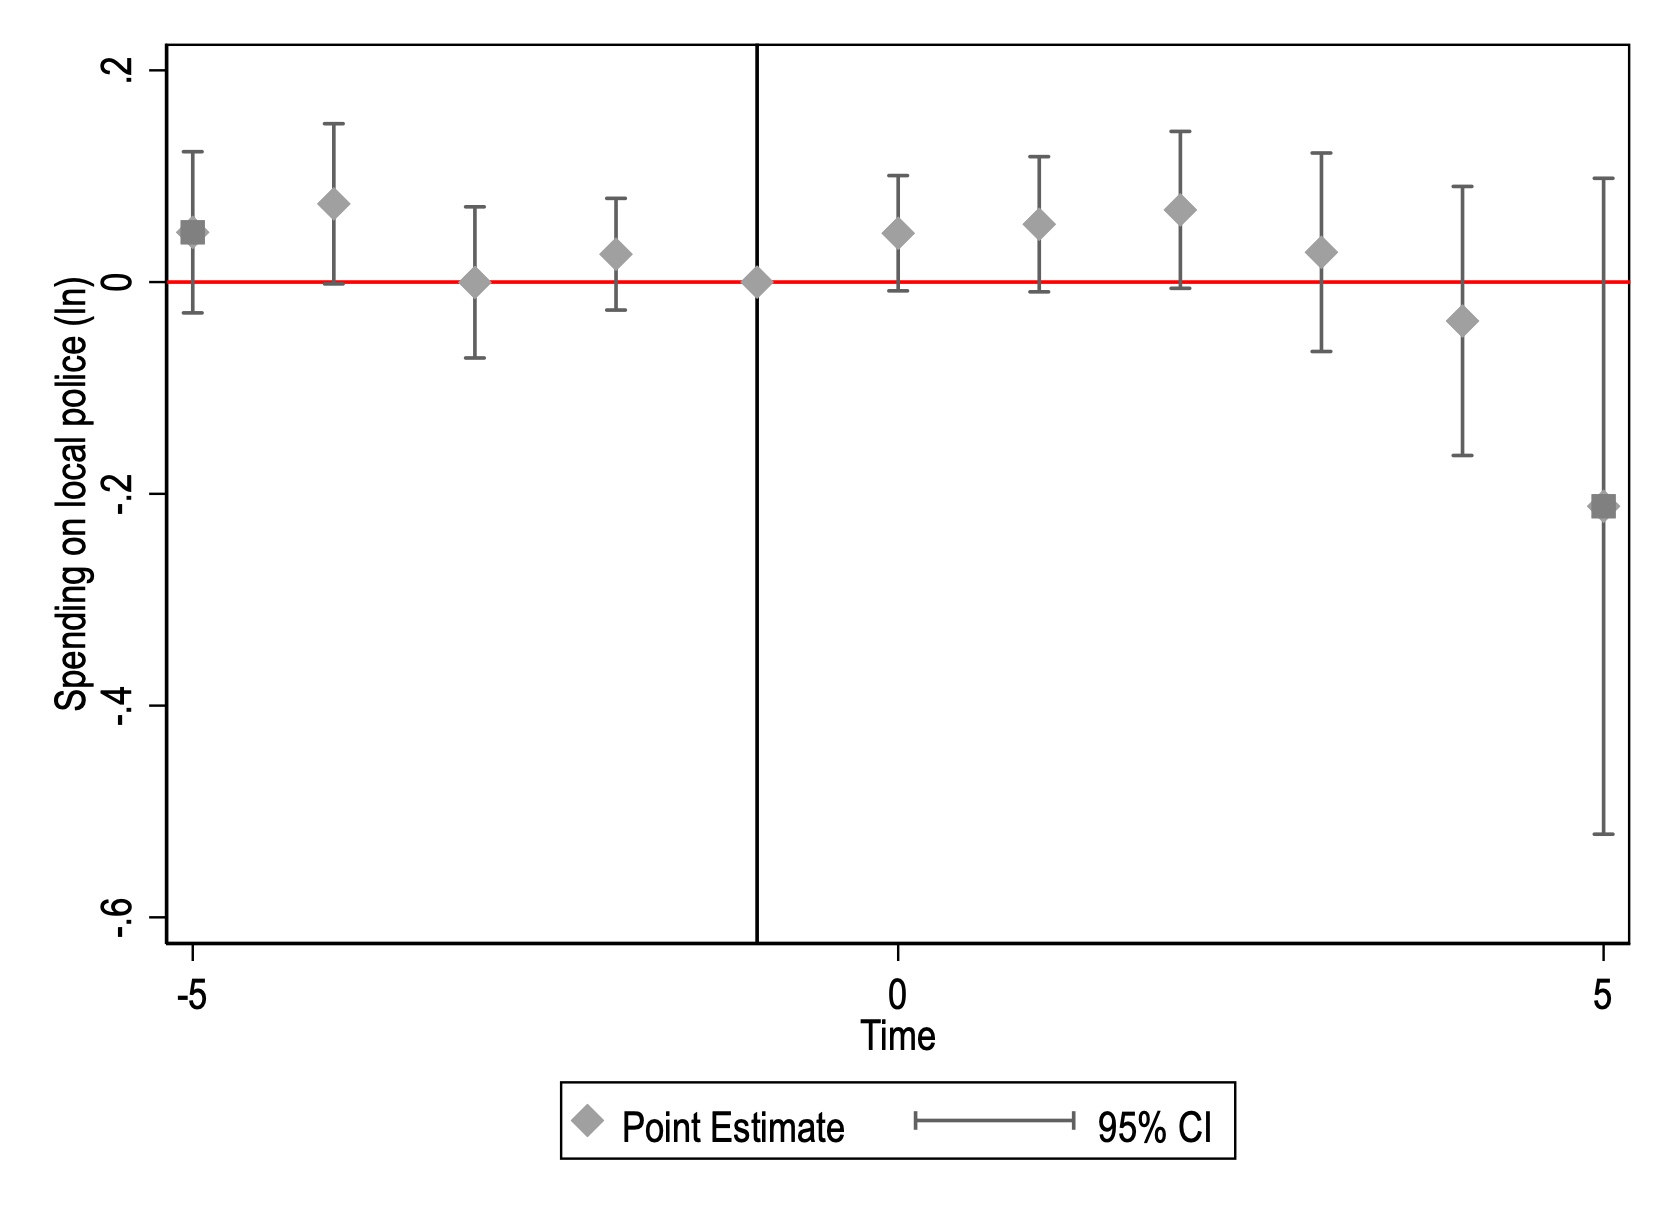
\includegraphics[width=\linewidth]{images/pop_5000/caseventdd_ln_q4_03_step1.jpg}
            \label{fig:caspolice}
        \end{minipage} &
        \begin{minipage}[t]{0.32\textwidth}
            \centering
            \caption{Culture, libraries, museums}
            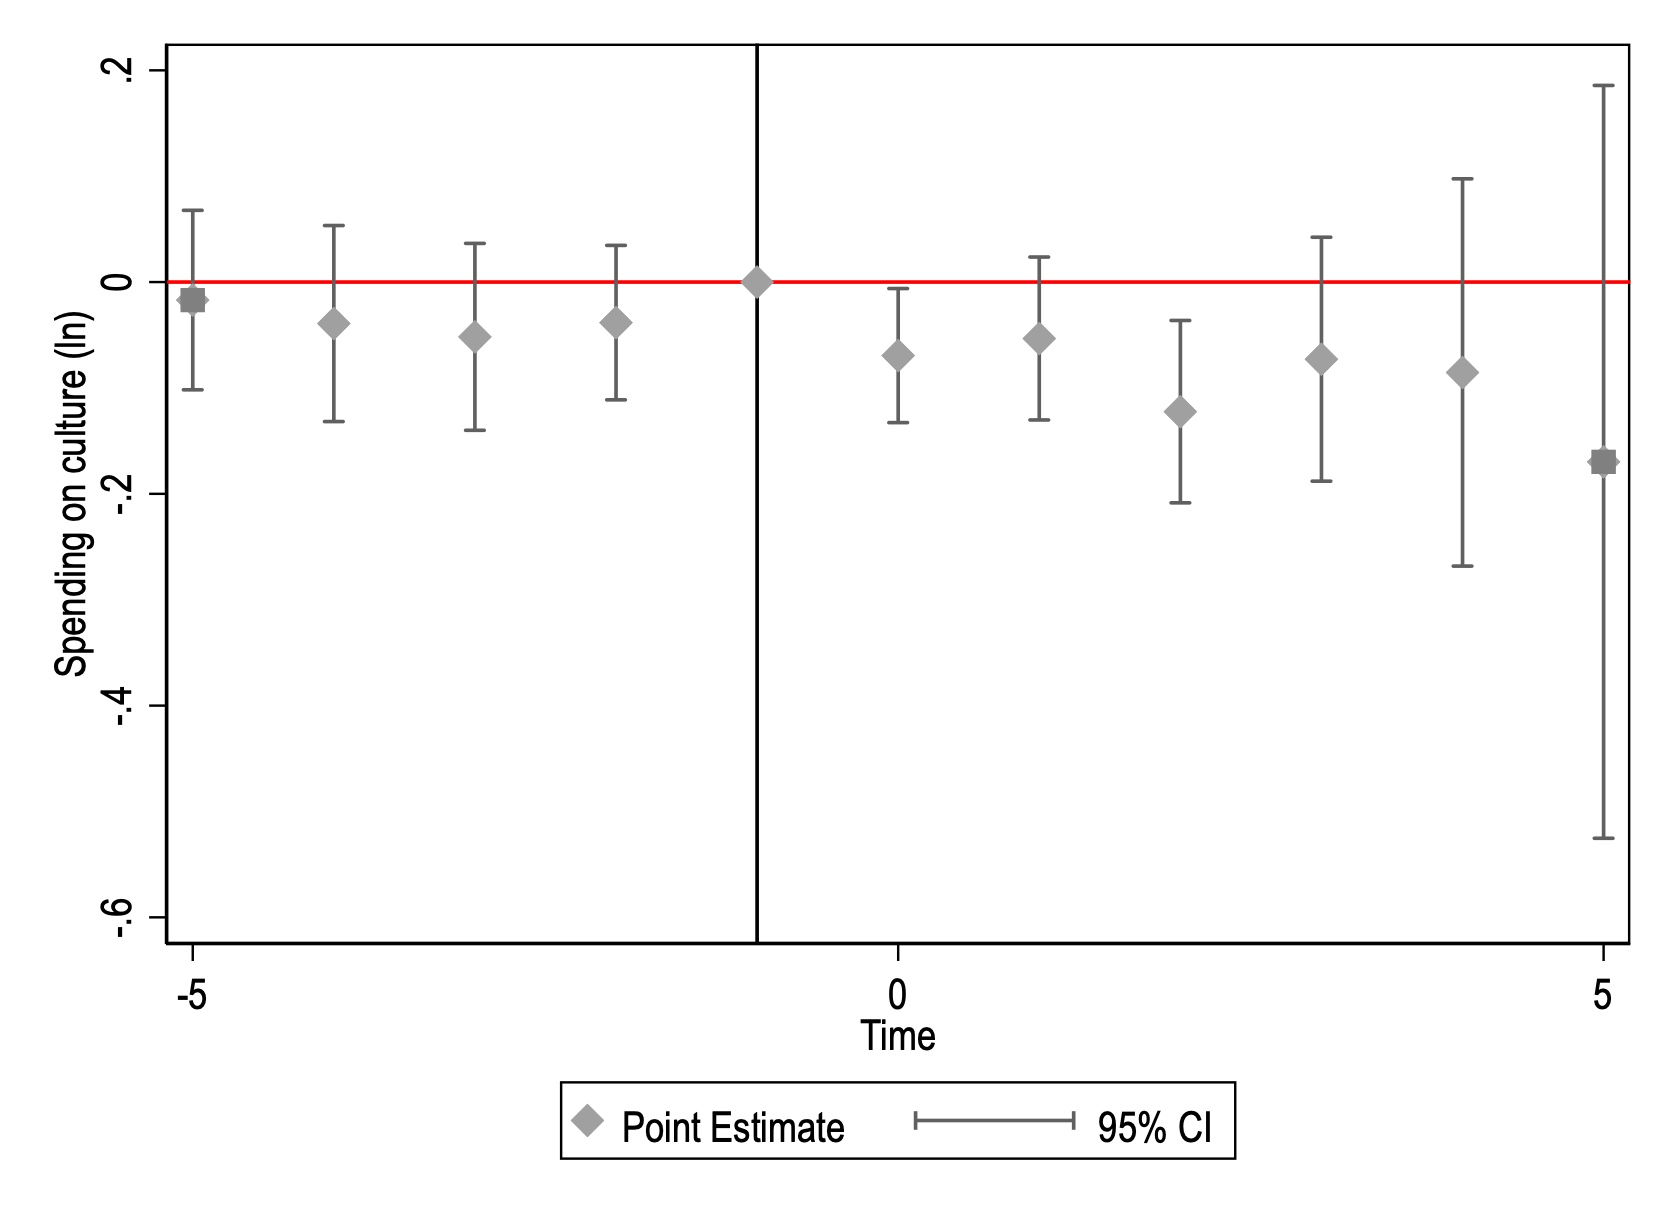
\includegraphics[width=\linewidth]{images/pop_5000/caseventdd_ln_q4_05_step1.jpg}
            \label{fig:casculture}
        \end{minipage} \\[10pt]

        \begin{minipage}[t]{0.32\textwidth}
            \centering
            \caption{Social services}
            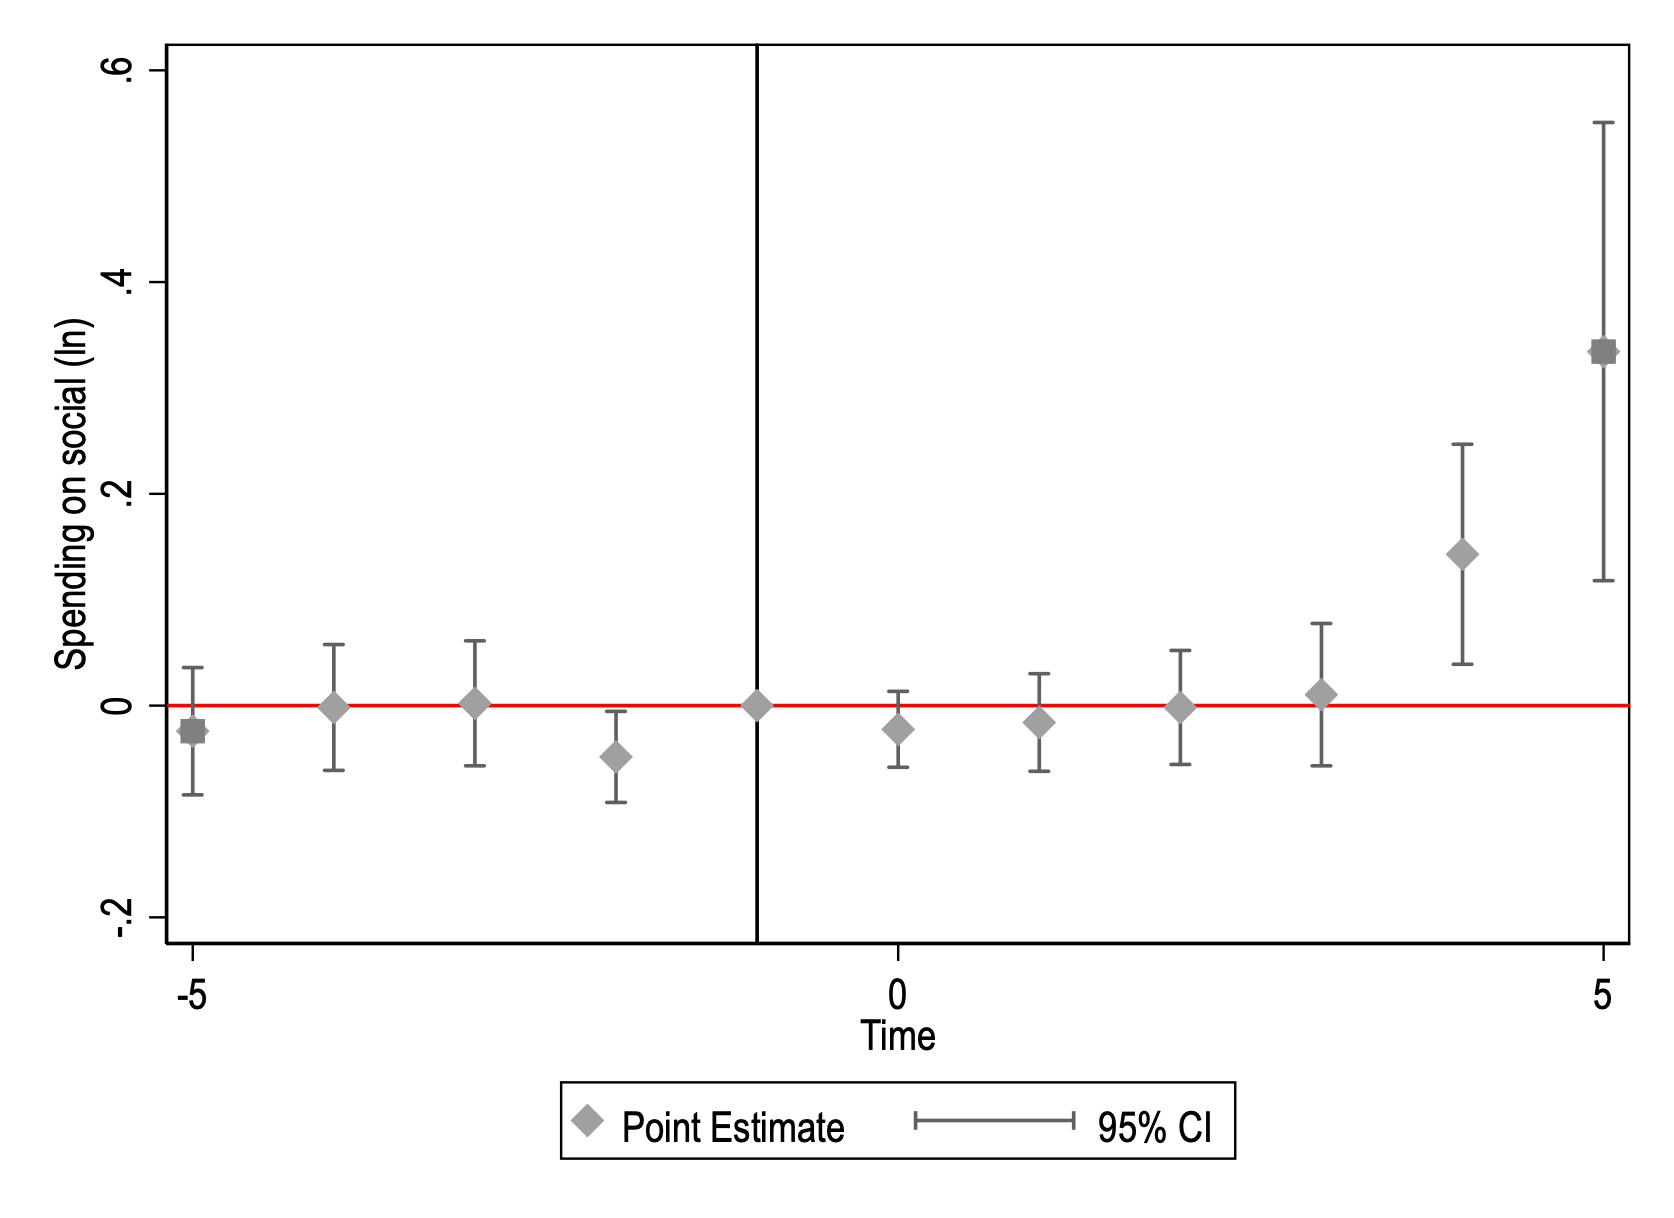
\includegraphics[width=\linewidth]{images/pop_5000/caseventdd_ln_q4_10_step1.jpg}
            \label{fig:cassocial_services}
        \end{minipage} &
        \begin{minipage}[t]{0.32\textwidth}
            \centering
            \caption{Education}
            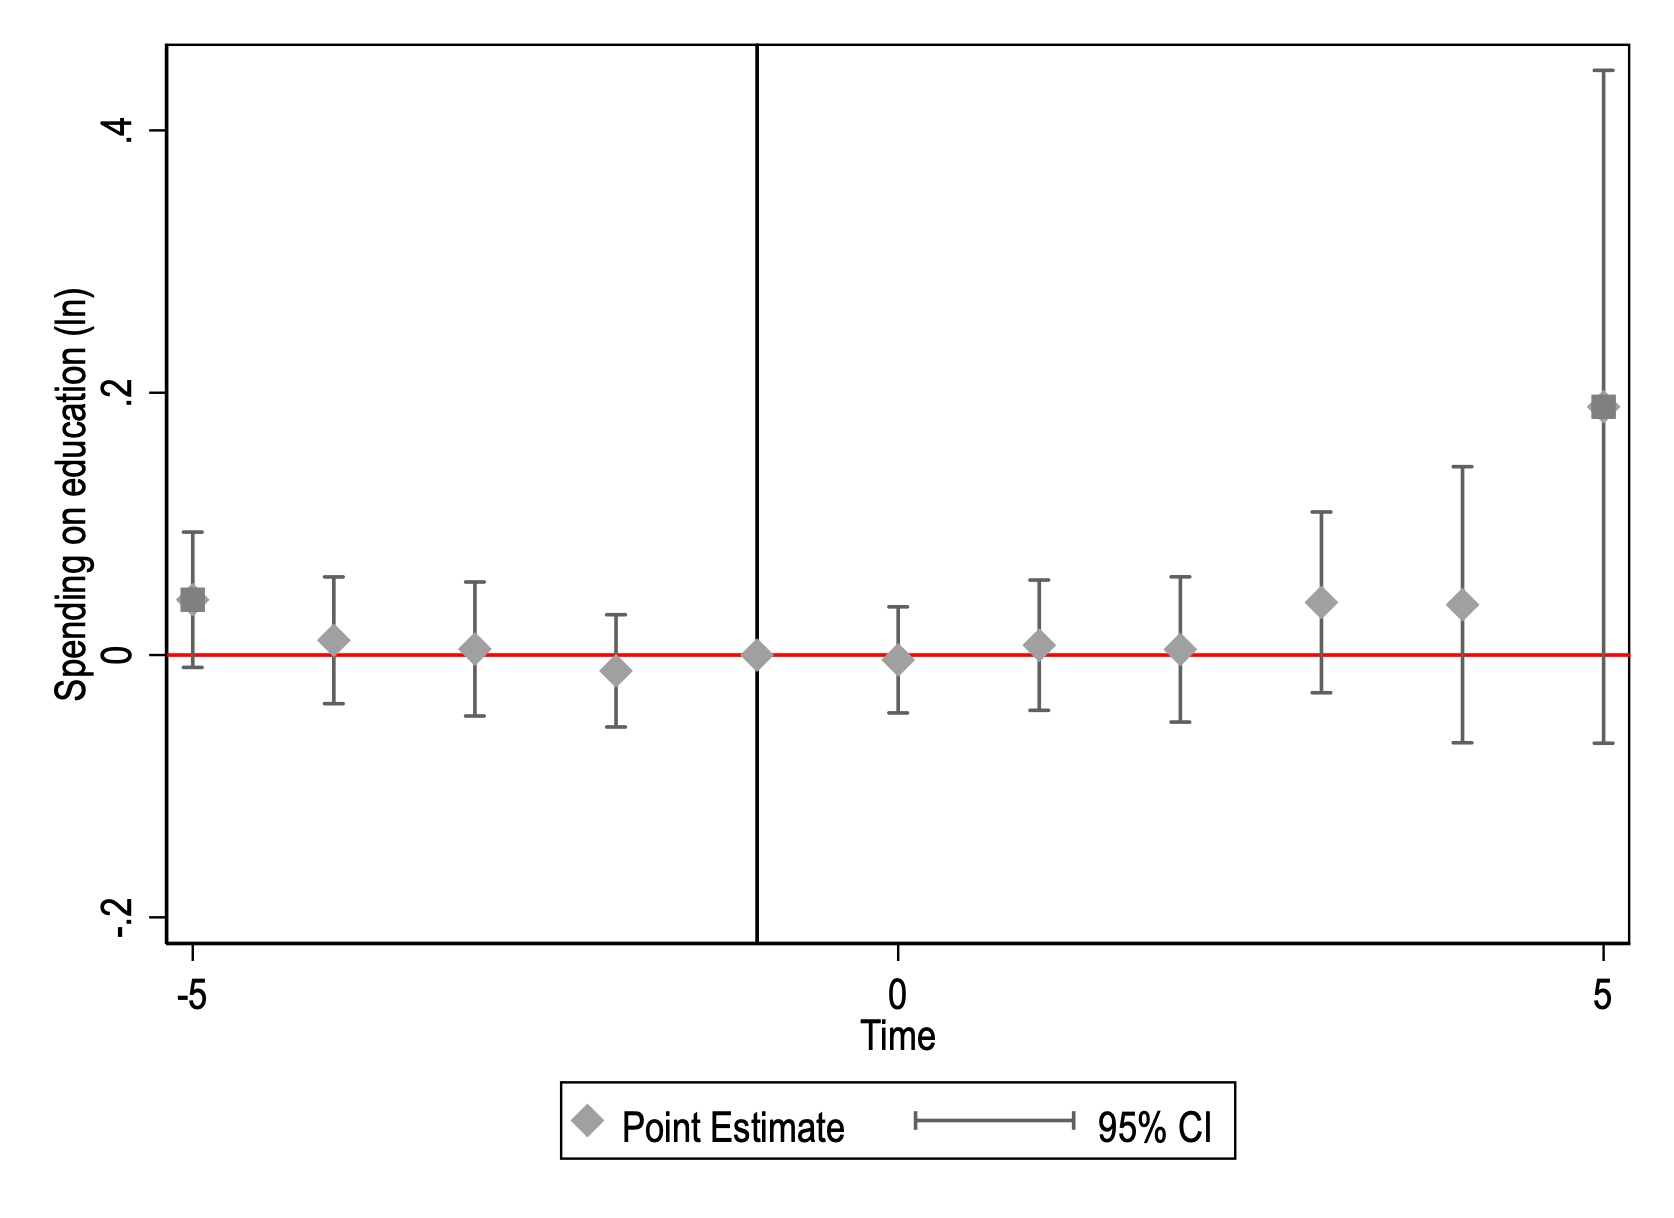
\includegraphics[width=\linewidth]{images/pop_5000/caseventdd_ln_q4_04_step1.jpg}
            \label{fig:caseducation}
        \end{minipage} &
        \begin{minipage}[t]{0.32\textwidth}
            \centering
            \caption{Economic development}
            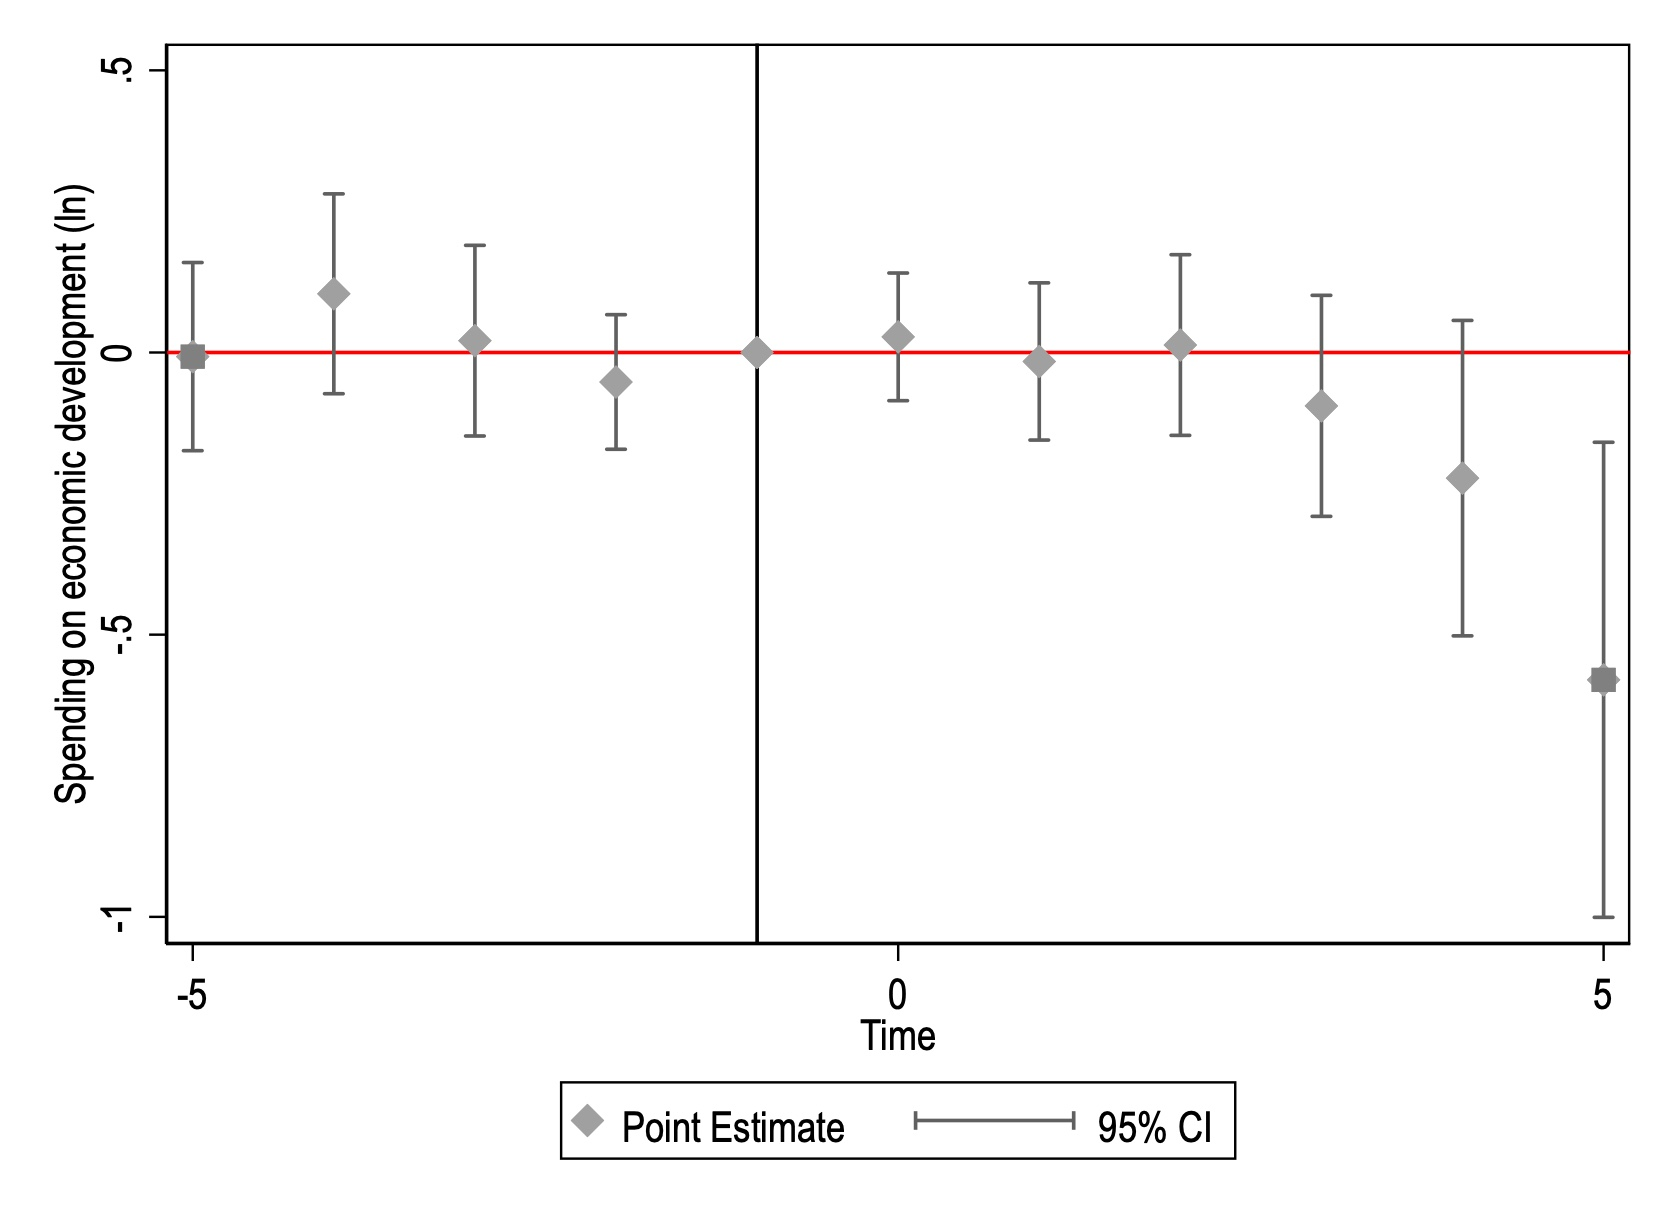
\includegraphics[width=\linewidth]{images/pop_5000/caseventdd_ln_q4_11_step1.jpg}
            \label{fig:casecodev}
        \end{minipage} \\[10pt]

        \begin{minipage}[t]{0.32\textwidth}
            \centering
            \caption{Production services}
            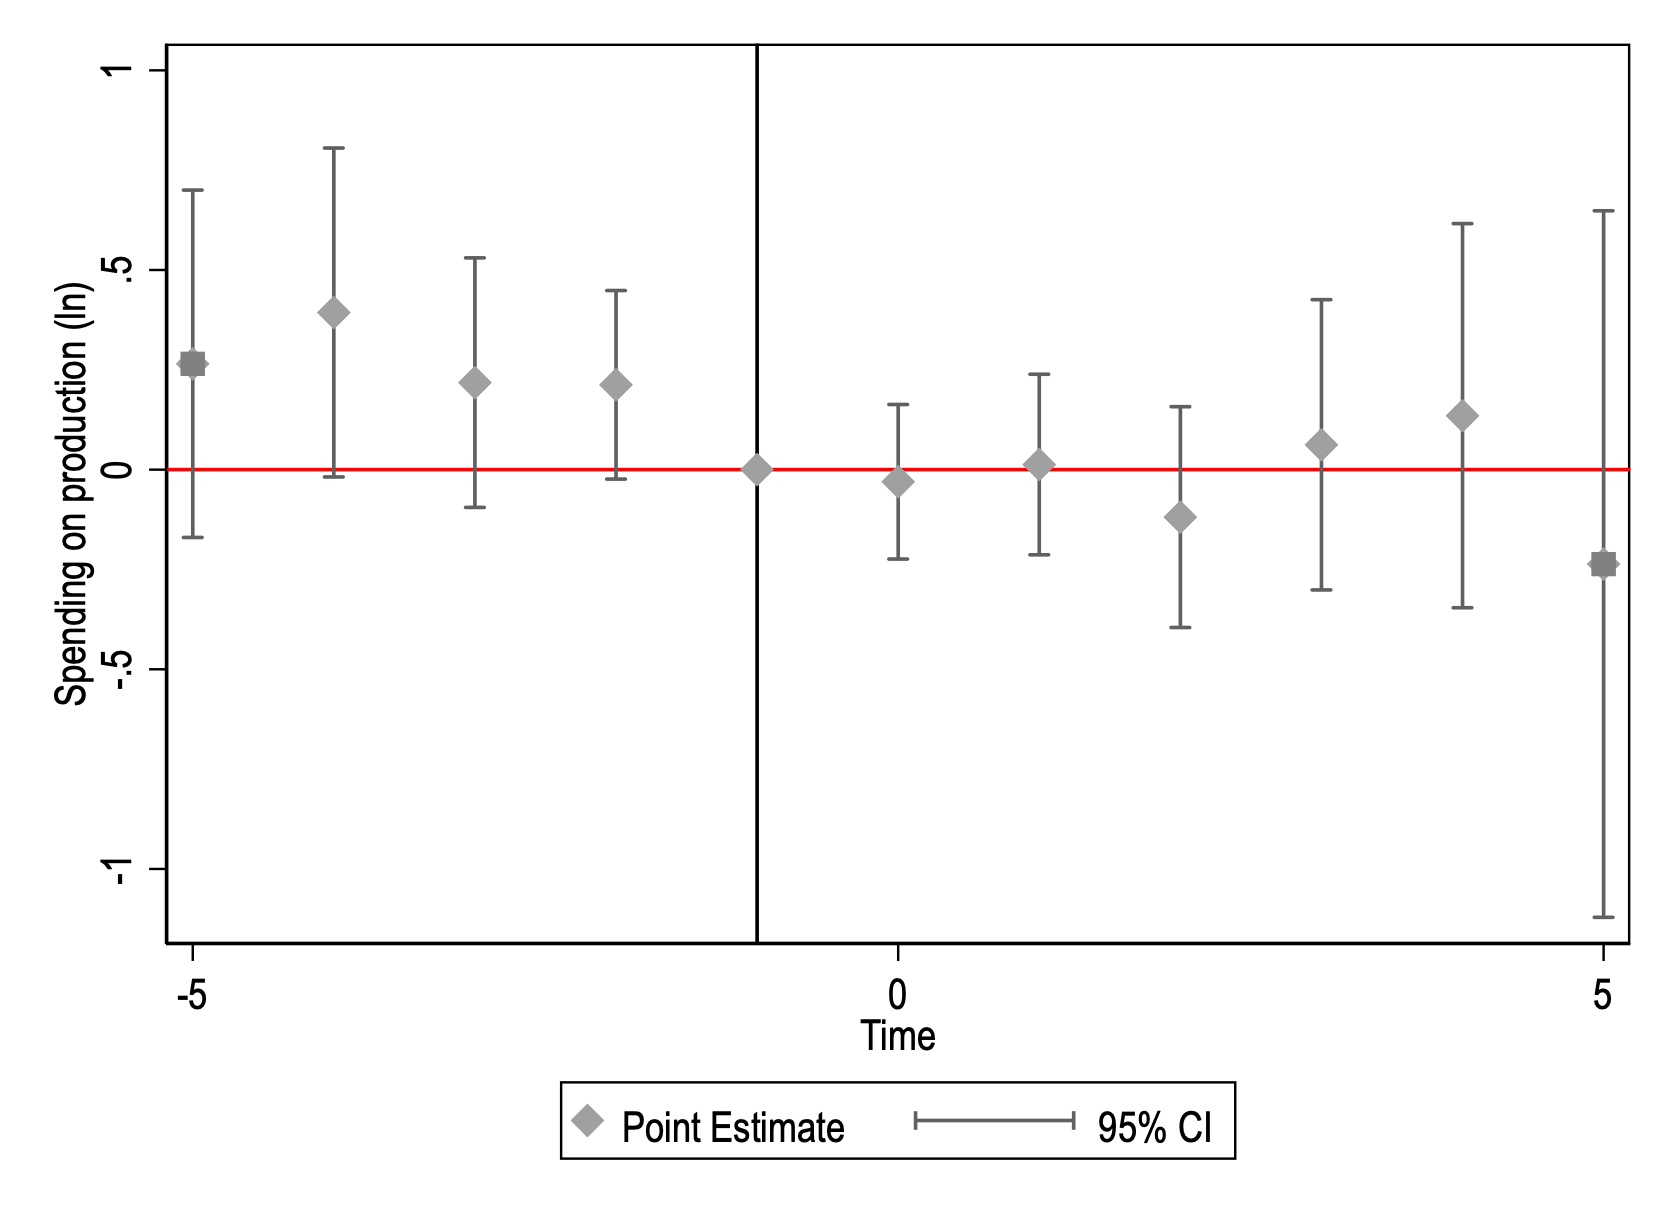
\includegraphics[width=\linewidth]{images/pop_5000/caseventdd_ln_q4_12_step1.jpg}
            \label{fig:cascproduction}
        \end{minipage} &
        \begin{minipage}[t]{0.32\textwidth}
            \centering
            \caption{Administrative services}
            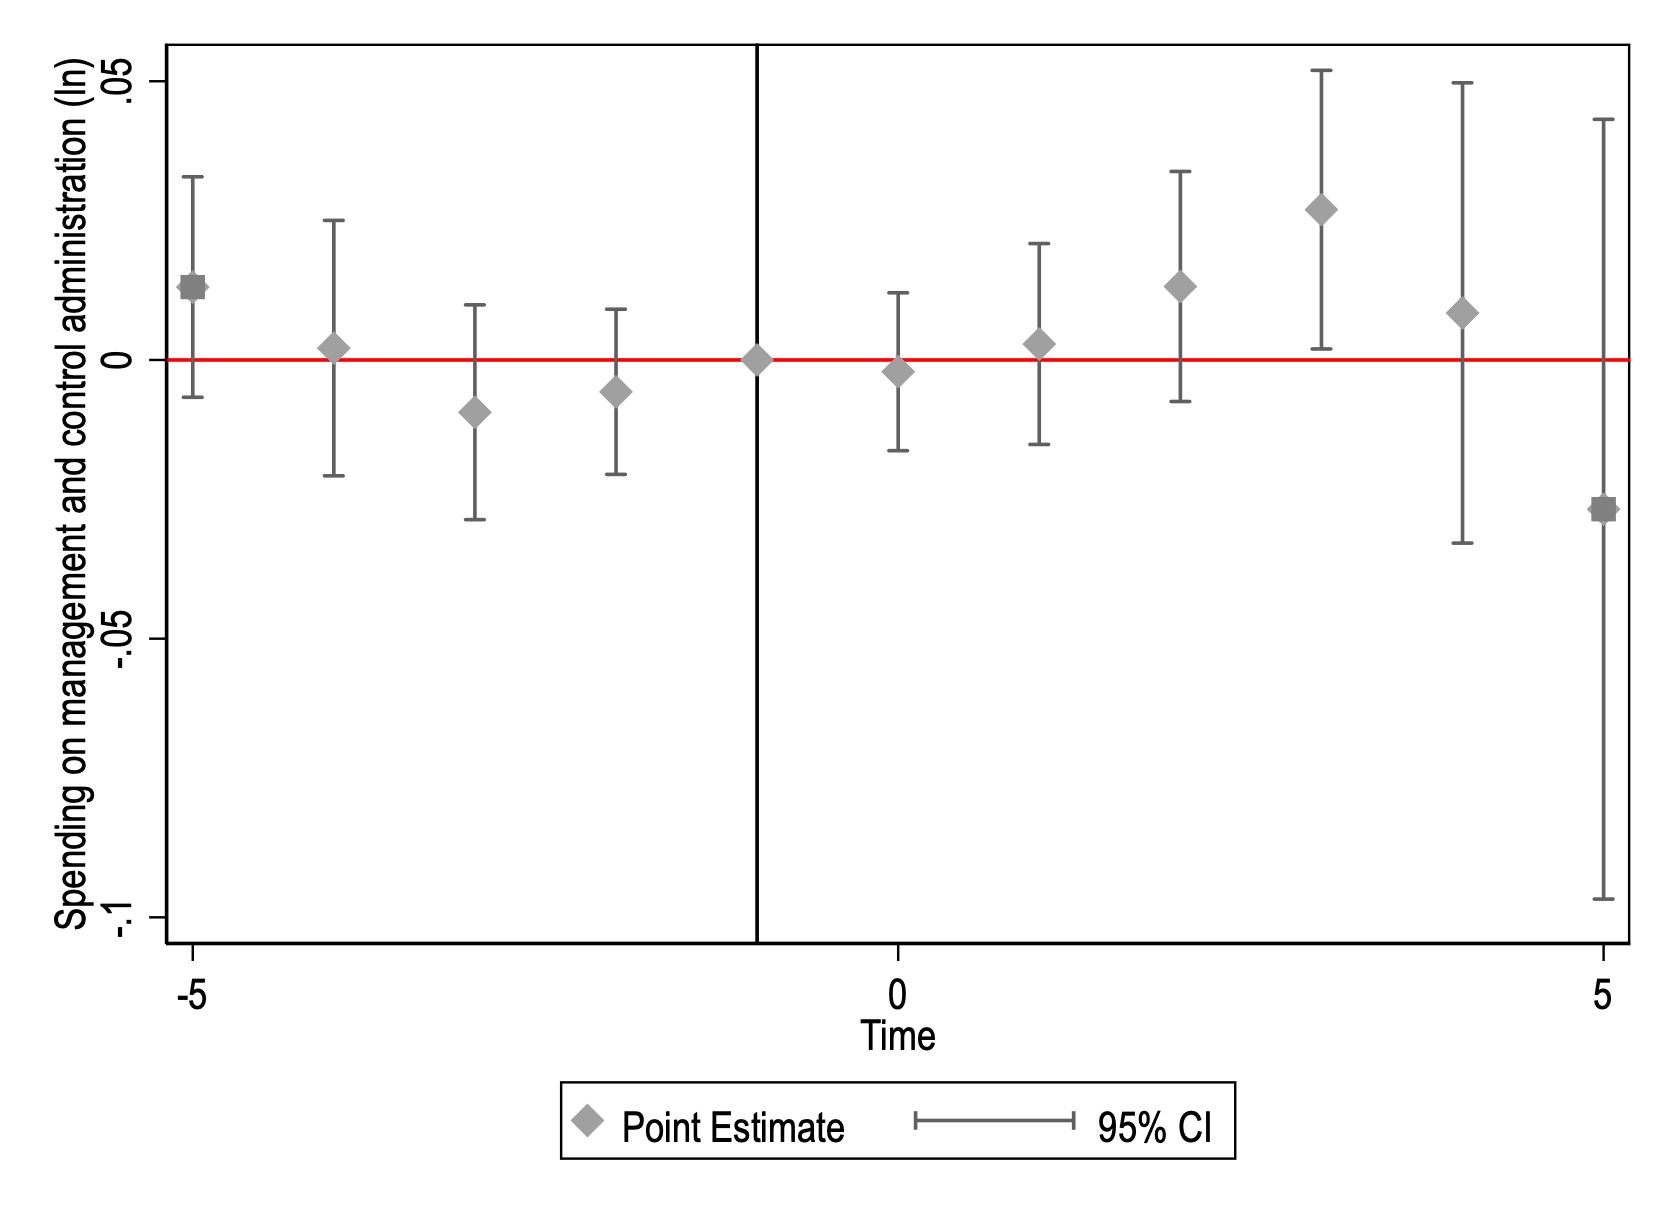
\includegraphics[width=\linewidth]{images/pop_5000/caseventdd_ln_q4_01_step1.jpg}
            \label{fig:casadministration}
        \end{minipage} &
        \begin{minipage}[t]{0.32\textwidth}
            \centering
            \caption{Environment, public parks, recycling}
            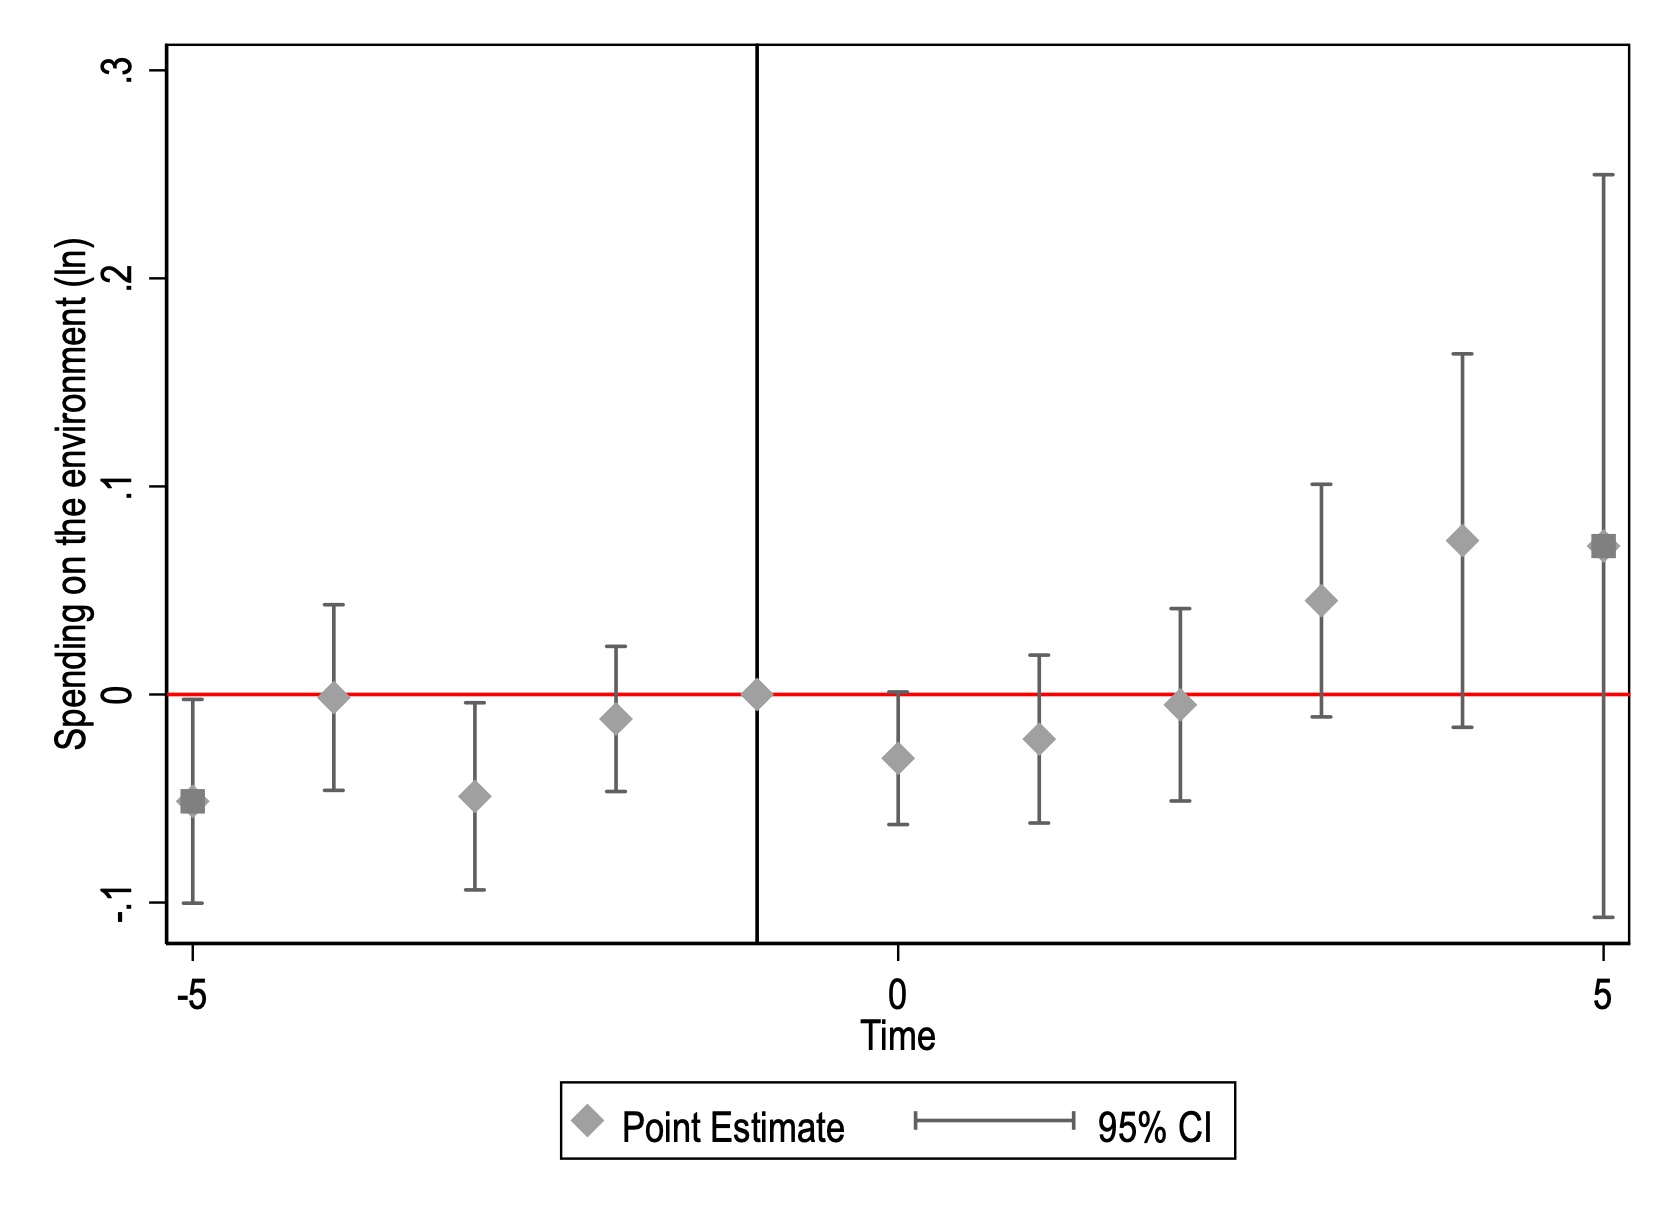
\includegraphics[width=\linewidth]{images/pop_5000/caseventdd_ln_q4_09_step1.jpg}
            \label{fig:casenvironment}
        \end{minipage}
    \end{tabular}
\end{figure}



\subsection{Cities with less than 10'000 people}


\justifying
\noindent
Results for smaller municipalities (population \(\leq\) 10'000) \\

\vspace{5}

\input{tables/pop_10000/descriptive stats sai.txt}
\input{tables/pop_10000/descriptive stats cas.txt}

\begin{figure}[ht]
\fontsize{7.2}{7.2}\selectfont
    \centering
\caption*{Effect of SAI centers on municipalities' public spending}
    \begin{tabular}{@{}ccc@{}}
        \begin{minipage}[t]{0.32\textwidth}
            \centering
            \caption{Total spending}
            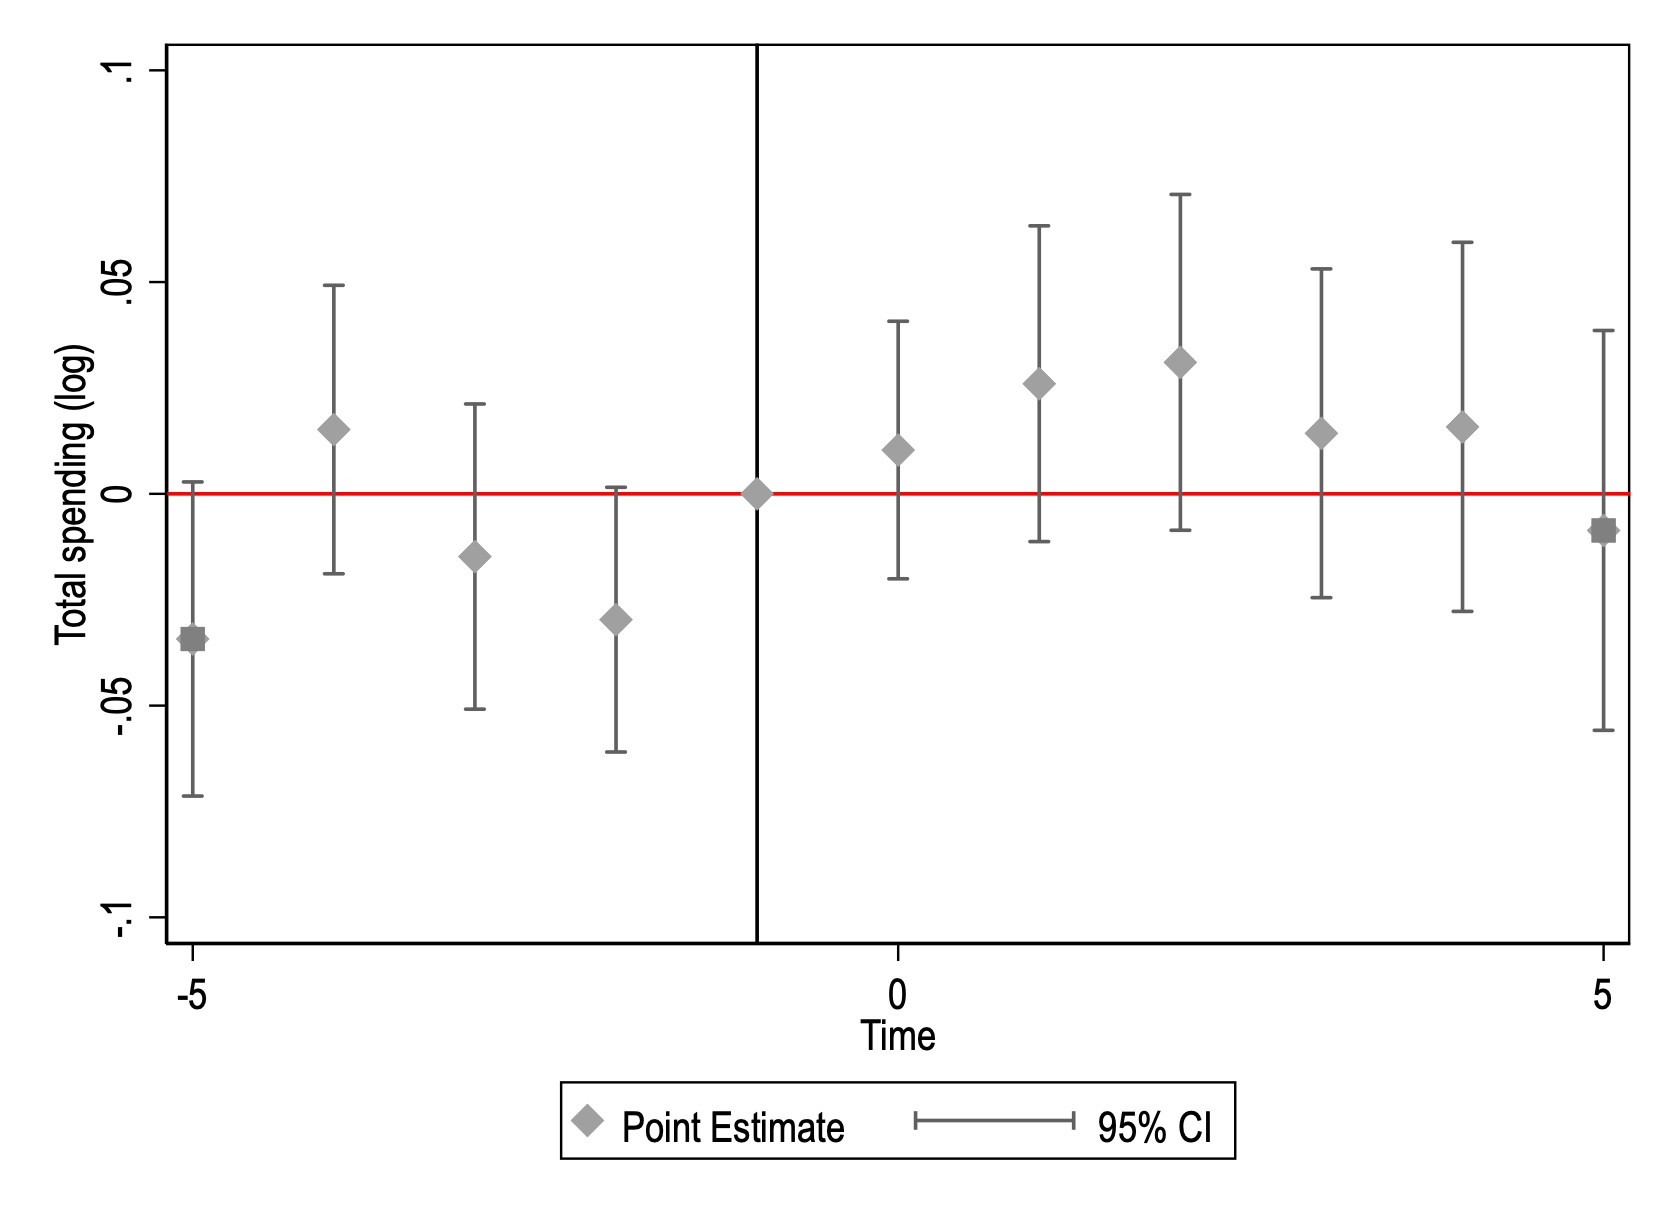
\includegraphics[width=\linewidth]{images/pop_10000/eventdd_ln_q4tot_step1.jpg}
            \label{fig:total_spending}
        \end{minipage} &
        \begin{minipage}[t]{0.32\textwidth}
            \centering
            \caption{Sport}
            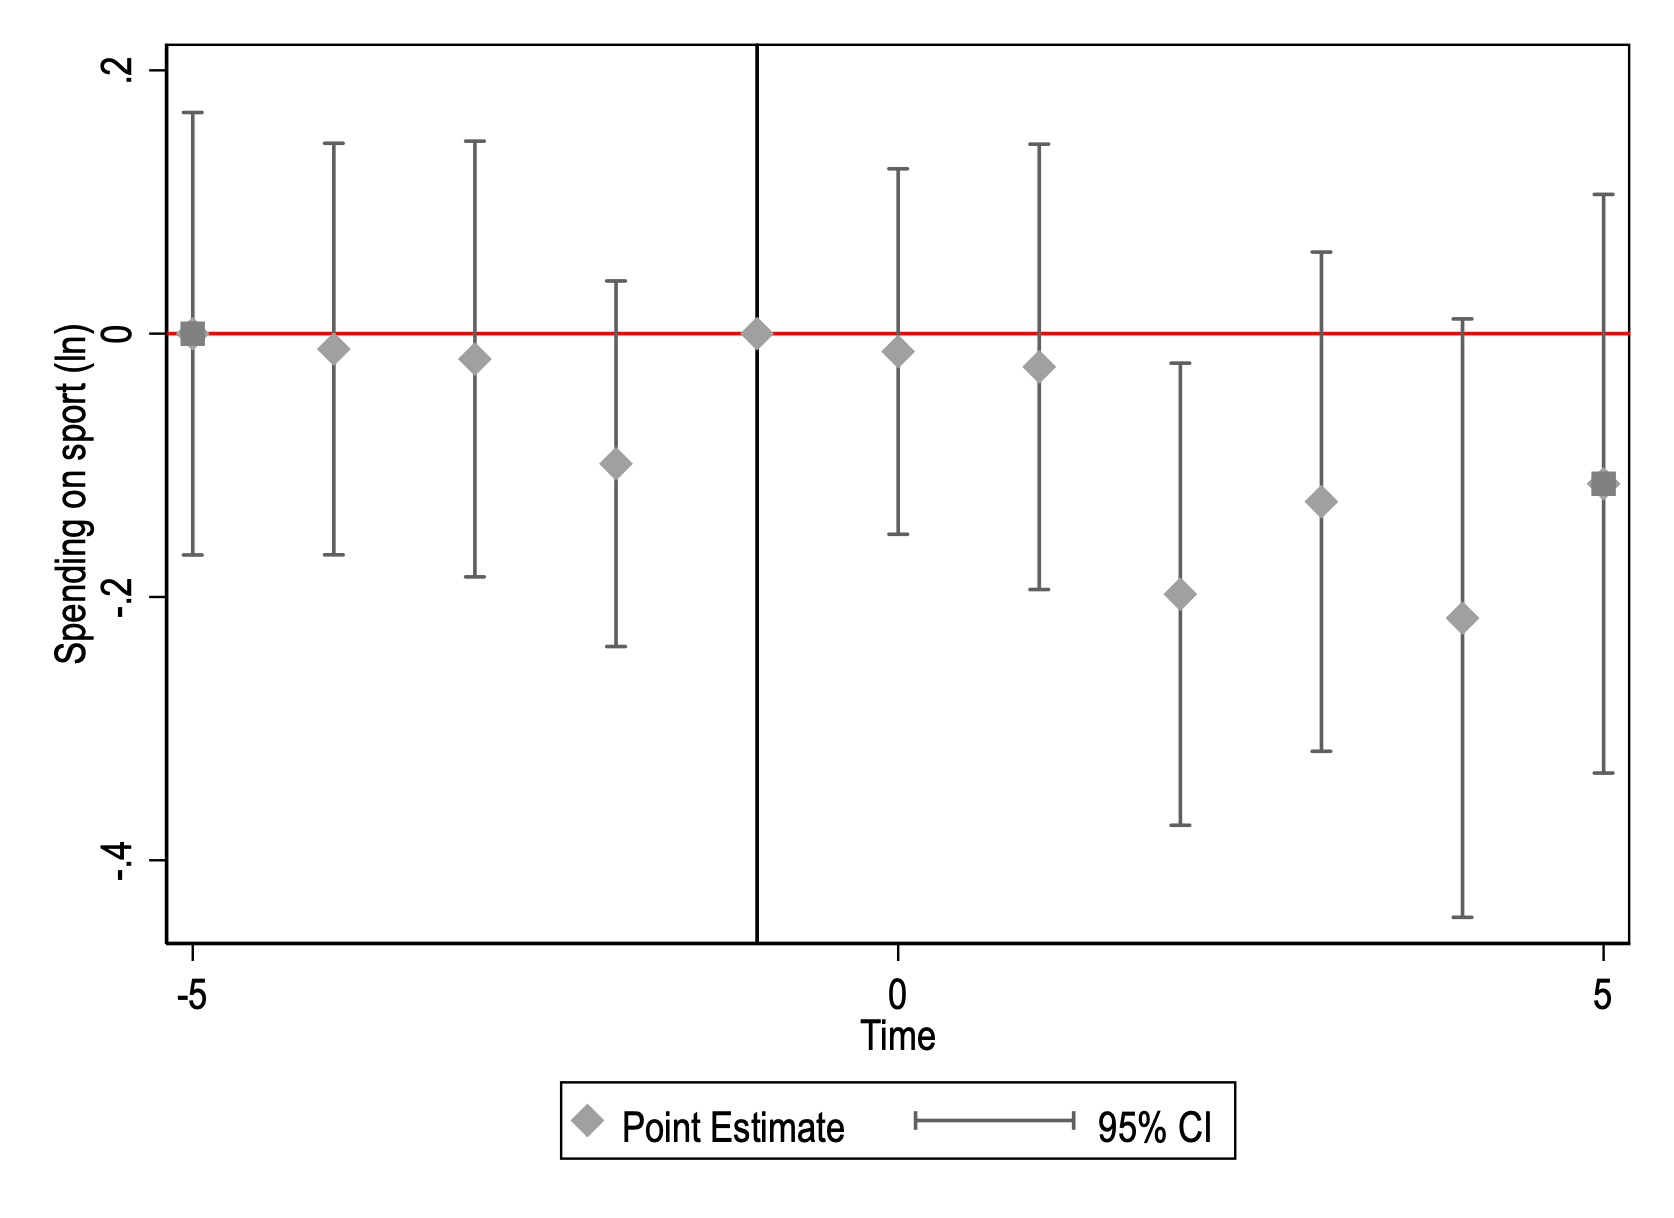
\includegraphics[width=\linewidth]{images/pop_10000/eventdd_ln_q4_06_step1.jpg}
            \label{fig:sport}
        \end{minipage} &
        \begin{minipage}[t]{0.32\textwidth}
            \centering
            \caption{Transport}
            \includegraphics[width=\linewidth]{images/pop_10000/eventdd_ln_q4_08_step1.jpg}
            \label{fig:transport}
        \end{minipage} \\[10pt]

        \begin{minipage}[t]{0.32\textwidth}
            \centering
            \caption{Justice}
            \includegraphics[width=\linewidth]{images/pop_10000/eventdd_ln_q4_02_step1.jpg}
            \label{fig:justice}
        \end{minipage} &
        \begin{minipage}[t]{0.32\textwidth}
            \centering
            \caption{Police}
            \includegraphics[width=\linewidth]{images/pop_10000/eventdd_ln_q4_03_step1.jpg}
            \label{fig:police}
        \end{minipage} &
        \begin{minipage}[t]{0.32\textwidth}
            \centering
            \caption{Culture, libraries, museums}
            \includegraphics[width=\linewidth]{images/pop_10000/eventdd_ln_q4_05_step1.jpg}
            \label{fig:culture}
        \end{minipage} \\[10pt]

        \begin{minipage}[t]{0.32\textwidth}
            \centering
            \caption{Social services}
            \includegraphics[width=\linewidth]{images/pop_10000/eventdd_ln_q4_10_step1.jpg}
            \label{fig:social_services}
        \end{minipage} &
        \begin{minipage}[t]{0.32\textwidth}
            \centering
            \caption{Education}
            \includegraphics[width=\linewidth]{images/pop_10000/eventdd_ln_q4_04_step1.jpg}
            \label{fig:education}
        \end{minipage} &
        \begin{minipage}[t]{0.32\textwidth}
            \centering
            \caption{Economic development}
            \includegraphics[width=\linewidth]{images/pop_10000/eventdd_ln_q4_11_step1.jpg}
            \label{fig:ecodev}
        \end{minipage} \\[10pt]

        \begin{minipage}[t]{0.32\textwidth}
            \centering
            \caption{Production services}
            \includegraphics[width=\linewidth]{images/pop_10000/eventdd_ln_q4_12_step1.jpg}
            \label{fig:production}
        \end{minipage} &
        \begin{minipage}[t]{0.32\textwidth}
            \centering
            \caption{Administrative services}
            \includegraphics[width=\linewidth]{images/pop_10000/eventdd_ln_q4_01_step1.jpg}
            \label{fig:administration}
        \end{minipage} &
        \begin{minipage}[t]{0.32\textwidth}
            \centering
            \caption{Environment, public parks, recycling}
            \includegraphics[width=\linewidth]{images/pop_10000/eventdd_ln_q4_09_step1.jpg}
            \label{fig:environment}
        \end{minipage}
    \end{tabular}
\end{figure}


\begin{figure}[ht]
\fontsize{7.2}{7.2}\selectfont
    \centering
\caption*{Effect of CAS centers on municipalities' public spending}
    \begin{tabular}{@{}ccc@{}}
        \begin{minipage}[t]{0.32\textwidth}
            \centering
            \caption{Total spending}
            \includegraphics[width=\linewidth]{images/pop_10000/caseventdd_ln_q4tot_step1.jpg}
            \label{fig:castotal_spending}
        \end{minipage} &
        \begin{minipage}[t]{0.32\textwidth}
            \centering
            \caption{Sport}
            \includegraphics[width=\linewidth]{images/pop_10000/caseventdd_ln_q4_06_step1.jpg}
            \label{fig:cassport}
        \end{minipage} &
        \begin{minipage}[t]{0.32\textwidth}
            \centering
            \caption{Transport}
            \includegraphics[width=\linewidth]{images/pop_10000/caseventdd_ln_q4_08_step1.jpg}
            \label{fig:castransport}
        \end{minipage} \\[10pt]

        \begin{minipage}[t]{0.32\textwidth}
            \centering
            \caption{Justice}
            \includegraphics[width=\linewidth]{images/pop_10000/caseventdd_ln_q4_02_step1.jpg}
            \label{fig:casjustice}
        \end{minipage} &
        \begin{minipage}[t]{0.32\textwidth}
            \centering
            \caption{Police}
            \includegraphics[width=\linewidth]{images/pop_10000/caseventdd_ln_q4_03_step1.jpg}
            \label{fig:caspolice}
        \end{minipage} &
        \begin{minipage}[t]{0.32\textwidth}
            \centering
            \caption{Culture, libraries, museums}
            \includegraphics[width=\linewidth]{images/pop_10000/caseventdd_ln_q4_05_step1.jpg}
            \label{fig:casculture}
        \end{minipage} \\[10pt]

        \begin{minipage}[t]{0.32\textwidth}
            \centering
            \caption{Social services}
            \includegraphics[width=\linewidth]{images/pop_10000/caseventdd_ln_q4_10_step1.jpg}
            \label{fig:cassocial_services}
        \end{minipage} &
        \begin{minipage}[t]{0.32\textwidth}
            \centering
            \caption{Education}
            \includegraphics[width=\linewidth]{images/pop_10000/caseventdd_ln_q4_04_step1.jpg}
            \label{fig:caseducation}
        \end{minipage} &
        \begin{minipage}[t]{0.32\textwidth}
            \centering
            \caption{Economic development}
            \includegraphics[width=\linewidth]{images/pop_10000/caseventdd_ln_q4_11_step1.jpg}
            \label{fig:casecodev}
        \end{minipage} \\[10pt]

        \begin{minipage}[t]{0.32\textwidth}
            \centering
            \caption{Production services}
            \includegraphics[width=\linewidth]{images/pop_10000/caseventdd_ln_q4_12_step1.jpg}
            \label{fig:cascproduction}
        \end{minipage} &
        \begin{minipage}[t]{0.32\textwidth}
            \centering
            \caption{Administrative services}
            \includegraphics[width=\linewidth]{images/pop_10000/caseventdd_ln_q4_01_step1.jpg}
            \label{fig:casadministration}
        \end{minipage} &
        \begin{minipage}[t]{0.32\textwidth}
            \centering
            \caption{Environment, public parks, recycling}
            \includegraphics[width=\linewidth]{images/pop_10000/caseventdd_ln_q4_09_step1.jpg}
            \label{fig:casenvironment}
        \end{minipage}
    \end{tabular}
\end{figure}


\end{document}